%% Template para dissertacao/tese na classe UFBAthesis
%% versao 1.0
%% (c) 2005 Paulo G. S. Fonseca
%% (c) 2012 Antonio Terceiro
%% (c) 2014 Christina von Flach
%% www.dcc.ufba.br/~flach/ufbathesis

%% Carrega a classe ufbathesis
%% Opcoes: * Idiomas
%%           pt   - portugues (padrao)
%%           en   - ingles
%%         * Tipo do Texto
%%           bsc  - para monografias de graduacao
%%           msc  - para dissertacoes de mestrado (padrao)
%%           qual - exame de qualificacao de mestrado
%%           prop - exame de qualificacao de doutorado
%%           phd  - para teses de doutorado
%%         * Media
%%           scr  - para versao eletronica (PDF) / consulte o guia do usuario
%%         * Estilo
%%           classic - estilo original a la TAOCP (deprecated) - apesar de deprecated, manter esse.
%%           std     - novo estilo a la CUP (padrao)
%%         * Paginacao
%%           oneside - para impressao em face unica
%%           twoside - para impressao em frente e verso (padrao)

% Atenção: Manter 'classic' na declaracao abaixo:
\documentclass[msc, classic, a4paper]{ufbathesis}

%% Preambulo:
\usepackage[utf8]{inputenc}

%\usepackage[authoryear]{natbib}
\usepackage{graphicx}
\usepackage{lipsum}
\usepackage{hyphenat}
\usepackage[usenames, dvipsnames, table]{xcolor}

\usepackage{pifont}
\usepackage{multirow}
\usepackage{listings}
\usepackage[portuguese, noend, plain, linesnumbered]{algorithm2e}
\usepackage{colortbl}
\usepackage{xfrac}
\usepackage[FIGTOPCAP]{subfigure}

\usepackage{adjustbox}
\usepackage{tabularx,ragged2e,booktabs}
\newcolumntype{L}{>{\RaggedRight\arraybackslash}X}

\usepackage{acronym}
\usepackage{float}
\usepackage{todonotes}
\usepackage{amssymb}
\usepackage{placeins}
\usepackage{arydshln}
\usepackage{pdflscape}

\presetkeys%
    {todonotes}%
    {inline,backgroundcolor=yellow}{}

\usepackage{blindtext}

\makeatletter
\DeclareRobustCommand{\element}[1]{\@element#1\@nil}
\def\@element#1#2\@nil{%
  \MakeLowercase{#1}%
  \if\relax#2\relax\else\MakeLowercase{#2}\fi}
\pdfstringdefDisableCommands{\let\element\@firstofone}
\makeatother

\renewcommand{\arraystretch}{1.3}

% Siglas
\acrodef{AM}[AM]{{Aprendizado de Máquina}}
\acrodef{DE}[DE] {{Distância Euclidiana}}
\acrodef{FCD}[FCD] {{\textit {Fluxo de Dados Contínuos}}}
\acrodef{DN}[DN] {{\textit {Detecção de Novidade}}}
\acrodef{RBF}[RBF] {{\textit {Rede de Função de Base Radial}}}

% Universidade
\university{Universidade Federal da Bahia}

% Endereco (cidade)
\address{Salvador}

% Instituto ou Centro Academico
\institute{Instituto de Matem\'{a}tica}

% Nome da biblioteca - usado na ficha catalografica
\library{Biblioteca Reitor Mac\^{e}do Costa}

% Programa de pos-graduacao
\program{Programa de P\'{o}s-Gradua\c{c}\~{a}o em Ci\^{e}ncia da Computa\c{c}\~{a}o}

% Area de titulacao
\majorfield{Ci\^{e}ncia da Computa\c{c}\~{a}o}

% Titulo da dissertacao
\title{Uso de Redes de Função de Base Radial e Cadeias de Markov para detecção online de mudanças de conceito em fluxos contínuos de dados}

% Data da defesa
% e.g. \date{19 de fevereiro de 2013}
\date{16 de Dezembro de 2019}
% e.g. \defenseyear{2013}
\defenseyear{2019}

% Autor
% e.g. \author{Jose da Silva}
\author{Ruivaldo Azevedo Lobão Neto}

% Orientador(a)
% Opcao: [f] - para orientador do sexo feminino
% e.g. \adviser[f]{Profa. Dra. Maria Santos}
\adviser{Ricardo Ara\'{u}jo Rios}

% Orientador(a)
% Opcao: [f] - para orientador do sexo feminino
% e.g. \coadviser{Prof. Dr. Pedro Pedreira}
% Comente se nao ha co-orientador
%\coadviser{Nome Completo do CO-ORIENTADOR}

%% Inicio do documento
\begin{document}

\pgcompfrontpage

%% Parte pre-textual
\frontmatter

\pgcomppresentationpage

%%%%%%%%%%%%%%%%%%%%%%%%%
% Ficha catalografica
%%%%%%%%%%%%%%%%%%%%%%%%%

%\authorcitationname{Silva, Mirlei Moura da } % e.g. Terceiro, Antonio Soares de Azevedo
%\advisercitationname{Sobrenome, Nome do ORIENTADOR} % e.g. Chavez, Christina von Flach Garcia
%\coadvisercitationname{Sobrenome, Nome do CO-ORIENTADOR} % e.g. Mendonca, Manoel Gomes de
%\catalogtype{Disserta\c{c}\~{a}o (Mestrado)} % e.g. ou ``Tese (Doutorado)''

%\catalogtopics{1. Primeira palavra-chave. 2. Segunda palavra-chave. 3. Terceira palavra-chave} % Listar palavras-chave do trabalho para a FICHA CATALOGRAFICA}, por exemplo, ``1. Complexidade Estrutural. 2. Qualidade de Software 3. Engenharia de Software''
%\catalogcdd{XXX.XX} % e.g.  XXX.XX (número nesse formato serah dado pela biblioteca)
%\catalogcdu{XXX.XX.XXX} % e.g.  XXX.XX.XXX (idem)
%\catalogingsheet

%%%%%%%%%%%%%%%%%%%%%
% Termo de aprovacaoo
%%%%%%%%%%%%%%%%%%%%%

% \approvalsheet{Salvador, 24 de Maio de 2019}{
%    \comittemember{Prof. Dr. Ricardo Araújo Rios}{UFBA}
%    %\comittemember{Profa. Dr...}{UFBA}
%    %\comittemember{Prof. Dr...}{USP}
% }
   % Para mestrado, apenas 3.
   % \comittemember{Prof. Dr. Professor 4}{Universidade HJKL}
   % \comittemember{Profa. Dra. Professora 5}{Universidade QWERTY}

%%%%%%%%%%%%%%%%%%%%%%%%%%%%%%%%%%%%%%%%
% Dedicatoria, Agradecimentos, Epigrafe
%%%%%%%%%%%%%%%%%%%%%%%%%%%%%%%%%%%%%%%%

% Comente para ocultar
% \begin{dedicatory}
%     Dedicatória...
% \end{dedicatory}

% Agradecimentos
% Se preferir, crie um arquivo `a parte e o inclua via \include{}
% \acknowledgements

% Epigrafe
% \begin{epigraph}[]{Provérbios 4:23}
% Sobre tudo o que se deve guardar, guarda o teu coração, porque dele procedem as fontes da vida.
% \end{epigraph}

%%%%%%%%%%%%%%%%%%%%%
% Resumo
%%%%%%%%%%%%%%%%%%%%%
\resumo

A quantidade de informações produzidas por sistemas computacionais tem crescido de forma acentuada nas últimas décadas.
Uma parcela expressiva dessas informações é produzida na forma de fluxos contínuos, que são sequências constantes e potencialmente infinitas de dados.
Esses fluxos são, em sua maioria, não-estacionários, podendo sofrer alterações na distribuição dos dados ou no contexto do processo gerador.
Estas alterações são denominadas mudanças de conceito e podem impactar negativamente a performance de modelos de aprendizado aplicados.
Para mitigar este problema, pesquisadores vêm desenvolvendo métodos especializados na detecção de mudanças de conceito.
Entretanto, os métodos propostos apresentam limitações ao serem aplicados em alguns cenários de fluxos contínuos como, por exemplo,
a necessidade de rotulação por especialistas e a incapacidade de atender às restrições de tempo de processamento e de uso dos recursos computacionais desses cenários.
Visando superar essas limitações, este trabalho apresenta um novo método de detecção de mudanças de conceito, denominado RBFChain, baseado em Redes de Função de Base Radial (RBF) e Cadeias de Markov.
Resumidamente, as redes RBF realizam, em sua camada intermediária, um processo de ativação que, implicitamente, produz grupos a partir das observações recebidas ao longo do tempo.
De maneira complementar, as cadeias de Markov permitem modelar as transições entre esses grupos.
Mudanças de conceito são, então, detectadas quando o grupo ativo é alterado e a probabilidade da transição, no modelo markoviano, excede um limiar.
O método apresentado se diferencia dos trabalhos existentes por detectar mudanças em tempo de execução, de forma computacionalmente eficiente e independente de rótulos.
Para avaliar o método RBFChain como um detector de mudanças de conceito viável, uma análise de sensibilidade, precisão e tolerância ao ruído foi realizada usando conjuntos de dados sintéticos,
e seus resultados foram comparados com os principais algoritmos disponíveis na literatura.
Além disso, a técnica foi aplicada a um problema real de classificação de fixações e sacadas na atividade de monitoramento ocular.
Com essa aplicação, foi possível investigar e propor uma solução para um problema relevante que envolve a área de Neurociência e Computação.
Os resultados obtidos com os conjuntos de dados sintéticos sugerem que o RBFChain é estatisticamente melhor ou equivalente aos principais detectores presentes na literatura.
Ademais, a técnica desenvolvida apresentou bons resultados quando aplicada ao problema de monitoramento ocular,
sendo capaz de classificar fixações e sacadas em tempo real e com precisão equivalente ao estado da arte.

% Palavras-chave do resumo em Portugues
\begin{keywords}
    Fluxo Contínuo de Dados. Mudança de Conceito. Rede de Função de Base Radial. Cadeia de Markov. Monitoramento Ocular.
\end{keywords}

\abstract

The amount of information produced by computer systems has grown dramatically in recent decades.
A significant share of this volume is produced as data streams, which are constant and potentially infinite sequences.
Most of these streams are non-stationary and may vary over time.
These changes are called concept drifts and can negatively impact the performance of applied learning models.
To mitigate this problem, researchers developed specialized methods for detecting concept drifts.
However, the proposed methods have limitations when applied in scenarios with data streams,
such as the need for expert labeling or the inability to meet the processing time and computational resource constraints of these scenarios.
This work proposes a new detection method based on Radial Basis Function Networks (RBF) and Markov Chains, called RBFChain.
RBF networks perform, in their intermediate layer, an activation process that implicitly produces groups of observations received over time.
Simultaneously, the Markov Chain models the transitions between groups in the formed cluster.
Concept drifts are detected when the active group of the cluster changes, and the probability of this transition in the Markov model exceeds a threshold.
The proposed method differs from existing works in that it detects changes at run time,  in a computationally efficient and independent of labels way.
To assess RBFChain as a viable concept drift detector, an analysis of sensitivity, accuracy, and noise tolerance was performed using synthetic datasets, and results were compared to the main algorithms available in the literature.
Also, the technique was applied to the fixation and saccade classification problem in eye-tracking: a relevant issue for different areas of knowledge, because many behavioral experiments use this information as an analysis factor.
Results with synthetic datasets suggest that RBFChain is statistically better or equivalent to the main detectors present in the literature.
Moreover, the developed method presented good results when applied to the eye-tracking problem, being able to classify fixations and saccades in real-time and with accuracy equivalent to the state of the art.

% Palavras-chave do resumo em Ingles
\begin{keywords}
    Data Stream. Concept Drift. Radial Basis Function Network. Markov Chain. Eye-tracking.
\end{keywords}

%%%%%%%%%%%%%%%%%%%
% Sumario / Indice
%%%%%%%%%%%%%%%%%%%

% Comente para ocultar
\tableofcontents

% Lista de figuras
% Comente para ocultar
\listoffigures

% Lista de tabelas
% Comente para ocultar
\listoftables

% Lista de algoritmos
\listofalgorithms

%% Parte textual
\mainmatter

% Eh aconselhavel criar cada capitulo em um arquivo separado, digamos
% "capitulo1.tex", "capitulo2.tex", ... "capituloN.tex" e depois
% inclui-los com:
% \include{capitulo1}
% \include{capitulo2}
% ...
% \include{capituloN}
%
% Importante:
% Use \xchapter{}{} ao inves de \chapter{}; se não quiser colocar texto antes do inicio do capitulo, use \xchapter{texto}{}.

%%%
\xchapter{Introdução}{} \label{introducao}

\section{Contexto e Motivação}

Nos últimos anos, o volume de dados produzidos por sistemas computacionais aumentou significativamente.
%
Esse crescimento foi favorecido por avanços tecnológicos recentes, como
a pervasividade dos dispositivos móveis,
a popularização das redes sociais e
a expansão da internet das coisas \cite{Cohen:BigData:2009:MSN:1687553.1687576}.
%
A dimensão desse aumento foi verificada por \citeonline{idc_report},
cujo trabalho estima que, até 2020,
a quantidade de informações produzidas anualmente irá aumentar de 4,4 zettabytes (trilhões de gigabytes) para 44 zettabytes.

Parte significativa dessas informações é produzida na forma de sequências ininterruptas e potencialmente infinitas \cite{Aggarwal:2006:DSM:1196418}.
%
Na literatura, sequências com essas características são denominadas Fluxos Contínuos de Dados (FCDs) e estão presentes em diversos domínios de aplicação como, por exemplo, monitoramento do mercado financeiro \cite{ZHOU:2015},
acompanhamento de tráfico rodoviário \cite{Wang:2015:EOV:2843092.2843464},
gerenciamento de redes de telecomunicação \cite{delattre2015method},
análise de sentimento em tempo real \cite{KRANJC2015187} e
sistemas de prevenção e identificação de intrusos \cite{KENKRE:PAI:COLACO:2015}.

Para extrair informações úteis dessa grande quantidade de dados,
pesquisadores têm aplicado técnicas da área de Aprendizado de Máquina (AM),
a qual estuda algoritmos que melhoram seu desempenho conforme ganham experiência \cite{Mitchell:1997:ML:541177}.
%
Entretanto, as estratégias tradicionais de Aprendizado de Máquina têm aplicação limitada para contextos com fluxos contínuos de dados,
pois nesses cenários os algoritmos devem atender a restrições de tempo de execução e de uso dos recursos computacionais \cite{bifet2009data}.

Além dessas limitações,
as técnicas de Aprendizado de Máquina,
quando aplicadas em contextos com fluxos contínuos,
também devem lidar com variações na distribuição dos dados ou no contexto do processo gerador.
%
Essas alterações são denominadas Mudanças de Conceito \cite{Gama:2010:KDD:1855075} e
a sua ocorrência pode impactar a acurácia do modelo.

Inicialmente, a atualização periódica dos modelos foi utilizada como estratégia para evitar a perda de acurácia causada por tais mudanças.
%
Contudo, esta solução é pouco sofisticada e computacionalmente custosa.
%
Diante disso, pesquisadores propuseram técnicas de detecção de mudanças de conceito baseadas no monitoramento da performance do modelo \cite{Gama:2014:SCD:2597757.2523813}.
%
Estes métodos identificam a ocorrência de mudanças com maior precisão, permitindo que o modelo de decisão seja atualizado somente quando necessário.
%
Exemplos de algoritmos baseados nesta abordagem, incluem:
DDM \cite{GamaMCR04}, EDDM \cite{EDDM},
ADWIN \cite{BifetG07}, ECDD \cite{Ross:2012:EWM:2076039.2076307},
PL \cite{Bach:PL:2008}, FCWM \cite{FCWM} e STEPD \cite{STEPD}.

Entretanto, as técnicas baseadas em monitoramento necessitam que o rótulo correto de cada exemplo esteja disponível.
%
Em muitos cenários, o tempo ou o custo para obter esses rótulos é proibitivo \cite{Aggarwal:2006:DSM:1196418}.
%
Consequentemente, foram desenvolvidos novos algoritmos independentes de rótulos.
Nestes métodos, a detecção se baseia na identificação de exemplos que não se enquadram na estrutura conhecida dos dados \cite{Spinosa:2007:OCA:1244002.1244107}.
%
Geralmente, essa análise é implementada com base em técnicas de agrupamento, detecção de \textit{outliers} ou medidas de dissimilaridade \cite{Ryu:Kantardzic:2012}.
%
Os seguintes algoritmos são exemplos desta abordagem:
OLINDDA \cite{Spinosa:2007:OCA:1244002.1244107},
MINAS \cite{Faria:2013:NDA:2480362.2480515},
ECSMiner \cite{Masud:2011:CNC:1978259.1978529} e
GC3 \cite{Sethi2016b:GC3}.

Todavia, segundo \citeonline{Aggarwal:2006:DSM:1196418},
as técnicas de detecção de mudanças de conceito presentes na literatura, ainda, apresentam limitações ao serem aplicadas em cenários com fluxos contínuos de dados.
%
Os algoritmos dependentes de rótulo se tornam inviáveis, por causa do custo e do tempo necessário para obter os rótulos corretos.
%
Enquanto as técnicas independentes têm dificuldade em atender às restrições de tempo de execução e de uso dos recursos computacionais desses cenários.

Visando superar essas limitações, esta dissertação propõe um novo método de detecção de mudanças de conceito, denominado RBFChain, baseado em Redes de Função de Base Radial (RBF) e Cadeias de Markov.
O método proposto se diferencia dos trabalhos existentes por detectar mudanças em tempo de execução, de forma computacionalmente eficiente e independente de rótulos.
A técnica desenvolvida foi avaliada através de dois experimentos.
O primeiro, analisou a acurácia e a performance do método utilizando dados sintéticos, e os resultados obtidos foram comparados com os principais algoritmos disponíveis na literatura.
O segundo, aplicou a técnica a um problema real de classificação de fixações e sacadas na atividade de monitoramento ocular, um problema relevante que envolve a área de Neurociência e Computação.

\section{Hipótese e Objetivo}

Com base nas observações citadas anteriormente, a seguinte hipótese foi formulada:

\begin{center}
\textit{``A aplicação de Redes de Função de Base Radial e Cadeias de Markov em fluxos contínuos de dados permite a detecção de mudanças de conceito em tempo de execução, de forma computacionalmente eficiente e independente de rótulos.''}
\end{center}

Assim, o objetivo principal deste trabalho é a validação dessa hipótese.
Para atingir este objetivo, um novo método de detecção de mudanças de conceito, baseado em Redes de Função de Base Radial e Cadeias de Markov, foi desenvolvido.
A técnica proposta foi validada através de dois experimentos.

O primeiro experimento utilizou dados sintéticos para realizar uma análise detalhada de sensibilidade, precisão e tolerância ao ruído, confrontando o método proposto com os principais algoritmos disponíveis na literatura.

O segundo experimento aplicou a técnica a um problema real de classificação de fixações e sacadas na atividade de monitoramento ocular, um relevante problema relacionado à área de Neurociência.

\section{Contribuições}

As principais contribuições desta dissertação são as seguintes:

\begin{itemize}
    \item Um novo método de detecção de mudanças de conceito, denominado RBFChain, baseado em Redes de Função de Base Radial (RBF) e Cadeias de Markov, que se diferencia por detectar mudanças em tempo de execução, de forma computacionalmente eficiente e independente de rótulos;
    \item Uma nova abordagem, baseada em uma versão adaptada do RBFChain, para o problema real de classificação de fixações e sacadas em atividades de monitoramento ocular.
    A abordagem proposta se diferencia por realizar a classificação em tempo de execução e apresentar acurácia semelhante ao estado da arte.
\end{itemize}

\section{Organização do trabalho}

O restante do texto está organizado da seguinte forma:
%
o Capítulo \ref{fundamentacao_teorica} apresenta o referencial teórico que fundamenta esta pesquisa e os trabalhos relacionados.
A solução proposta é apresentada em detalhes no Capítulo \ref{rbfchain}.
A configuração dos experimentos, os critérios de avaliação e os resultados obtidos são apresentados no Capítulo \ref{experimentos_e_resultados}.
Por fim, as conclusões da dissertação e os trabalhos futuros são apresentados no Capítulo \ref{conclusoes_e_trabalhos_futuros}.

\xchapter{Fundamentação Teórica}{} \label{fundamentacao_teorica}
\section{Considerações Iniciais}

Este capítulo apresenta os conceitos que fundamentaram o desenvolvimento desta dissertação e discute os trabalhos relacionados encontrados na literatura.
As duas primeiras seções abordam a aplicação de Aprendizado de Máquina em Fluxos Contínuos de Dados (Seção \ref{sec:fluxos_continuos_am}) e o fenômeno Mudança de Conceito (Seção \ref{sec:mudanca_de_conceito}).
As duas seções seguintes detalham as Redes de Função de Base Radial (RBF) (Seção \ref{sec:rbf}) e as Cadeias de Markov (Seção \ref{sec:markov}).
Por fim, os trabalhos relacionados são discutidos (Seção \ref{sec:trabalhos_relacionados}) e as considerações finais do capítulo apresentadas.

\section{Fluxos Contínuos de Dados e Aprendizado de Máquina}
\label{sec:fluxos_continuos_am}

Fluxos Contínuos de Dados (FCDs) podem ser definidos como sequências ininterruptas e potencialmente infinitas de eventos \cite{Aggarwal:2006:DSM:1196418}.
%
Nestes fluxos, os eventos ocorrem em alta frequência, sendo necessário processá-los em tempo de execução.
%
Além disso, por serem de tamanho potencialmente ilimitado, não é possível armazená-los de forma permanente em memória.
%

As características dos fluxos contínuos de dados implicam as seguintes restrições aos algoritmos que os processam \cite{bifet2009data}:
%
\begin{itemize}
    \item É impossível armazenar todos os dados do fluxo. Somente uma pequena parcela pode ser processada e armazenada, enquanto o restante é descartado;
    \item A velocidade de chegada dos eventos exige que sejam processados em tempo de execução;
    \item A distribuição dos dados pode mudar com o tempo. Assim, os dados do passado podem se tornar irrelevantes ou mesmo prejudiciais para a descrição dos conceitos atuais.
\end{itemize}

A área de Aprendizado de Máquina (AM) estuda algoritmos que melhoram o seu desempenho conforme ganham experiência \cite{Mitchell:1997:ML:541177}.
%
Esses algoritmos se dividem em duas categorias principais:
%
não supervisionados (agrupamento ou \textit{clustering}) e supervisionados (classificação ou regressão).
%
Algoritmos de ambas as categorias foram adaptados para que pudessem ser aplicados em cenários com fluxos contínuos de dados.
%
As principais características de cada categoria e as especializações propostas serão discutidas a seguir.

As técnicas não supervisionadas realizam o agrupamento automático de dados segundo o seu grau de semelhança.
Essas técnicas têm como objetivo a formação de grupos com alta similaridade intragrupo e baixa similaridade intergrupo \cite{Jain:1988:ACD:46712}.
Os seguintes algoritmos são exemplos de técnicas não supervisionadas para cenários em lote:
K-Means \cite{Lloyd:2006:LSQ:2263356.2269955},
DBSCAN \cite{Ester:1996:DAD:3001460.3001507},
PAM \cite{kaufman:clustering1990} e
OPTICS \cite{Ankerst:1999:OOP:304181.304187}.

De acordo com \citeonline{Gama:2010:KDD:1855075}, a principal dificuldade ao aplicar técnicas não supervisionadas em cenários com fluxos contínuos é a manutenção da consistência e qualidade dos grupos formados, conforme novos dados são observados.
Portanto, é necessário que os algoritmos atuem de forma incremental, evoluindo os grupos formados ao longo do tempo \cite{Barbara:2002:RCD:507515.507519}.
Sendo assim, foram desenvolvidos métodos não supervisionados especializados para fluxos contínuos de dados.
Os seguintes trabalhos são exemplos dessas especializações:
CluStream \cite{Aggarwal:2003:FCE:1315451.1315460},
StreamKM++ \cite{Ackermann:2012:SCA:2133803.2184450},
DenStream \cite{Cao:Feng:Ester},
D-Stream \cite{Chen:Tu} e ClusTree \cite{Kranen:2011:CIM:2134350.2134352}.

Os algoritmos supervisionados realizam predições para novos exemplos utilizando um modelo criado a partir de uma base de treinamento \cite{Kotsiantis:2007:SML:1566770.1566773}.
Se a predição é categórica, entende-se como um problema de classificação.
Se a predição resulta em um valor numérico, trata-se de uma tarefa de regressão.
Exemplos de algoritmos supervisionados para cenários em lote, incluem:
árvores de decisão \cite{Breiman:Classification_Regression_Trees},
métodos baseados em regras,
redes neurais e máquinas de vetores suporte (SVM) \cite{Vapnik1998}.

Segundo \citeonline{Gama:2010:LDS:1951990},
as técnicas supervisionadas tradicionais não podem ser aplicadas a contextos com fluxos contínuos de dados,
pois estes métodos não contemplam as severas restrições de uso de memória e de tempo de execução desses cenários.
%
Dessa forma,
novos algoritmos supervisionados foram propostos para esses contextos \cite{Domingos:2000:MHD:347090.347107, Bifet:2013:EDS:2480362.2480516, Wang:2003:MCD:956750.956778, Aggarwal:2004:DCD:1014052.1014110, Gama:2003:ADT:956750.956813}.

As especializações mencionadas buscam atender às restrições de uso de memória e de tempo de execução dos contextos com fluxos contínuos de dados.
Contudo, não consideram que na maioria desses cenários as informações são geradas de forma não estacionária, e que a distribuição dos dados ou o contexto do processo gerador podem sofrer variações, alterando os resultados esperados.
Na literatura, essas variações são denominadas mudanças de conceito e a sua ocorrência pode impactar a acurácia da técnica aplicada \cite{Gama:2010:KDD:1855075}.

% Nesta dissertação, considera-se que os dados são obtidos a partir de fluxos contínuos de dados com ocorrência de mudanças de conceito.
% Na próxima seção, o fenômeno mudança de conceito será discutido em detalhes.

\section{Mudança de Conceito}
\label{sec:mudanca_de_conceito}

Técnicas de Aprendizado de Máquina aplicadas a cenários com fluxos contínuos de dados devem ser capazes de lidar com alterações na distribuição dos dados ou no contexto do processo gerador.
Essas alterações são denominadas Mudanças de Conceito (\textit{Concept Drift} ou \textit{Concept Shift}, em inglês) e podem alterar os resultados esperados (conceitos-alvo) dos algoritmos, prejudicando sua acurácia \cite{Widmer:1996:LPC:226791.226798}.

Na literatura, é comum utilizar a Teoria Bayesiana de Decisão \cite{Duda:2000:PC:954544} para descrever a tarefa de classificação.
Esta descrição será utilizada como base para formalização do fenômeno de mudança de conceito.

Sendo $X \in \mathbb{R}^p$ uma instância em um espaço $p$-dimensional de atributos e $X \in c_i$ onde $c_1$, $c_2$, \ldots, $c_k$ é o conjunto de classes,
o classificador ótimo para classificar $x \rightarrow c_i$ é determinado a partir das probabilidades a priori das classes $P(c_i)$ e pela função de densidade de probabilidade condicionada às classes $p(X|c_i), i = 1, \ldots, k$.
É possível definir um conceito como um conjunto de probabilidades a priori e condicionais das classes, como mostra a Equação \ref{eq:conceito}:

\begin{equation} \label{eq:conceito}
    S = \{(P(c_1), P(X|c_1)), (P(c_2), P(X|c_2)), ..., (P(c_k), P(X|c_k))\}
\end{equation}

Ainda segundo a Teoria Bayesiana, a classificação de uma instância $X$ baseada na máxima probabilidade a posteriori pode ser obtida através da Equação \ref{eq:classificacao}:

\begin{equation} \label{eq:classificacao}
    p(c_i|X) = \frac{p(c_i) * p(X|c_i)}{p(X)}
\end{equation}

Assim, é possível afirmar que há mudança de conceito entre os instantes $t_0$ e $t_1$ se

\begin{equation} \label{eq:3}
    {\exists}X : p_{t_0}(X, c) \ne p_{t_1}(X, c)
\end{equation}

onde $p_{t_0}$ e $p_{t_1}$ denotam as distribuições de probabilidades conjuntas nos instantes $t_0$ e $t_1$, respectivamente,
para $X$ e $c$ \cite{Gama:2014:SCD:2597757.2523813}.
Em outras palavras, um conjunto de dados possui resultados esperados legítimos em $t_0$, mas este mesmo conjunto passa a ter resultados esperados diferentes, também legítimos, em $t_1$ \cite{Kolter:2007:DWM:1314498.1390333}.

De acordo com \citeonline{Gama:2014:SCD:2597757.2523813}, as mudanças de conceito podem ser categorizadas como virtuais ou reais.
As mudanças virtuais são causadas por alterações na probabilidade a priori das classes, $P(c)$, e não alteram os conceitos-alvo.
Enquanto que as mudanças de conceito reais surgem a partir de alterações na probabilidade a posteriori, $p(c|X)$, e modificam os resultados esperados.
Os dois tipos de mudança de conceito estão representados na Figura \ref{fig:real_and_virtual_concept_drift}.

\begin{figure}[H]
\begin{center}
    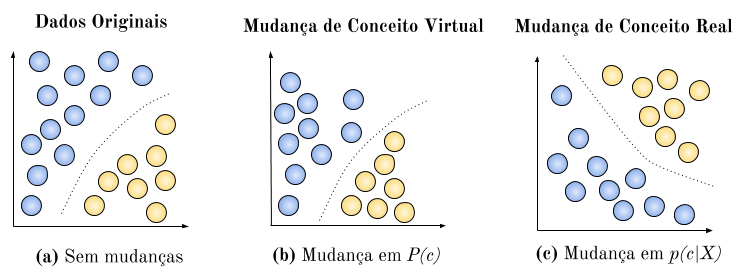
\includegraphics[scale=0.8]{imagens/concept_drift.png}
    \caption{Mudança de Conceito Virtual vs. Mudança de Conceito Real}
    \label{fig:real_and_virtual_concept_drift}
\end{center}
\end{figure}

Conforme \citeonline{Zliobaite:2010}, as mudanças de conceito podem ocorrer de forma abrupta, gradual, incremental ou recorrente.
A Figura \ref{fig:concept_drift_patterns} ilustra estes padrões,
utilizando círculos na cor azul para representar o conceito \textit{A} e círculos na cor bege para o conceito \textit{B}:

\begin{figure}[H]
\begin{center}
    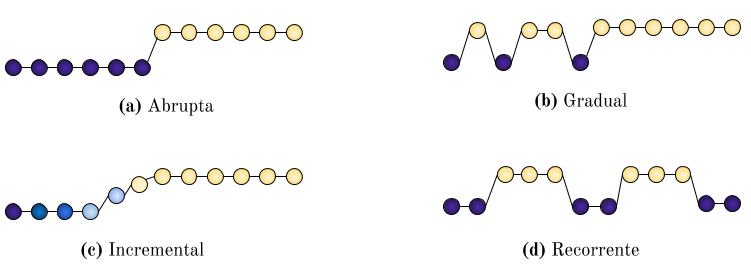
\includegraphics[scale=0.8]{imagens/concept_drift_patterns.png}
    \caption{Padrões de ocorrência de Mudanças de Conceito}
    \label{fig:concept_drift_patterns}
\end{center}
\end{figure}

\begin{itemize}
    \item Na mudança abrupta, o conceito \textit{A} é repentinamente substituído pelo conceito \textit{B} (Figura \ref{fig:concept_drift_patterns} (a)).
    
    \item Na mudança gradual, ocorre uma transição mais suave entre os conceitos \textit{A} e \textit{B}. Inicialmente, eventos pertencentes a ambos os conceitos coexistem. Com o passar do tempo, os eventos pertencentes ao conceito \textit{A} diminuem de frequência, até pararem de ocorrer. Por fim, os eventos pertencentes a \textit{B} se tornam predominantes (Figura \ref{fig:concept_drift_patterns} (b)).
    
    \item A mudança incremental descreve a evolução de um único conceito ao longo do tempo. Essa evolução pode ser discretizada como uma sequência de conceitos consecutivos. Nesta sequência, cada conceito intermediário difere pouco dos seus conceitos antecessor e sucessor. Portanto, as mudanças são notáveis apenas à longo prazo (Figura \ref{fig:concept_drift_patterns} (c)).
    
    \item A mudança recorrente acontece quando um conceito anteriormente ativo reaparece após um determinado período de tempo. Contudo, não se trata de uma sazonalidade periódica, pois não é evidente o momento no qual o conceito voltará a ser ativo (Figura \ref{fig:concept_drift_patterns} (d)).
\end{itemize}

O método de detecção proposto neste trabalho é capaz de identificar mudanças de conceito sob qualquer padrão de ocorrência e, por ser independente de rótulos, considera todas mudanças de conceito detectadas como reais.

% Na próxima subseção, será apresentada a terminologia do fenômeno mudança de conceito.

\subsection{Terminologia}

O fenômeno mudança de conceito tem sido estudado em diferentes comunidades de pesquisa, incluindo Mineração de Dados,
Aprendizado de Máquina, Estatística e Recuperação de Informação \cite{Zliobaite:2010}.
Contudo, o tema apresenta diferentes nomeclaturas em cada comunidade.
Na Tabela \ref{tbl:taxonomy} são listados os termos correspondentes a mudança de conceito em cada área de pesquisa.


\begin{table}[ht]
    \caption{Terminologia - Mudança de Conceito \cite{Zliobaite:2010}}
    \label{tbl:taxonomy}
    \centering
    
    \begin{tabularx}{\textwidth}{ l l }
    \toprule
    Área & Termos \\
    \midrule
    Mineração de Dados                  & Mudança de Conceito                        \\
    Aprendizado de Máquina              & Mudança de Conceito, Mudança de Covariável \\
    Computação Evolucionária            & Ambiente Evolutivo, Ambiente em Mudança    \\
    IA e Robótica                       & Ambiente Dinâmico                          \\
    Estatística, Séries Temporais      & Não Estacionário                           \\
    Recuperação de Informação           & Evolução Temporal                          \\
    \bottomrule
    \end{tabularx}
\end{table}

Outra fonte comum de equívocos são os termos detecção de \textit{outliers}, detecção de novidade, detecção de \textit{change points} e detecção de mudanças de conceito.
Estes termos são muitas vezes utilizados de forma indistinta, mas, para o contexto deste trabalho, é importante distingui-los.

As técnicas para detecção de \textit{outliers} têm como objetivo identificar padrões de dados em desacordo com o comportamento esperado. Estes padrões são geralmente classificados como anomalias ou ruídos \cite{Chandola:2009:ADS:1541880.1541882}.

Os métodos para detecção de novidade identificam padrões ainda não observados, mas que se enquadram no comportamento esperado.
Estes métodos se diferenciam das técnicas para detecção de \textit{outliers} pois os novos padrões são incorporados ao modelo \cite{Chandola:2009:ADS:1541880.1541882}.

As estratégias para detecção de \textit{change points} identificam variações abruptas de valor, que podem representar transições entre estados, em séries temporais unidimensionais estacionárias \cite{Aminikhanghahi:2017:SMT:3086013.3086037}.

Por fim,  cabe definir o que é detecção de mudanças de conceito.
Este termo abrange técnicas que monitoram a distribuição dos dados ou indicadores produzidos pelas técnicas de aprendizado aplicadas, com o objetivo de identificar variações que possam impactar a acurácia do modelo em uso \cite{Gama:2014:SCD:2597757.2523813}.

% Na próxima subseção, os algoritmos para detecção de mudança de conceito serão discutidos.

\subsection{Algoritmos para Detecção de Mudanças de Conceito}

Os algoritmos para detecção de mudanças de conceito caracterizam e quantificam as mudanças de conceito através da delimitação dos instantes ou intervalos de tempo em que as mudanças ocorrem \cite{Basseville:1993:DAC:151741}.

Esses algoritmos se dividem em duas categorias, conforme a necessidade de rotulação dos dados \cite{Zliobaite:2010}:

\begin{description}
    \item[Algoritmos Explícitos/Supervisionados] Dependem da rotulação dos dados por um especialista.
    Estes rótulos são utilizados no cálculo de medidas de performance como taxa de erro e acurácia, que são monitoradas ao longo do tempo.
    Mudanças de conceito são sinalizadas quando essas medidas atingem um limite previamente definido.

    \item[Algoritmos Implícitos/Não Supervisionados] Independem da rotulação por especialistas.
    As mudanças de conceito são detectadas a partir do monitoramento de características dos próprios dados ou de indicadores produzidos pelas técnicas de aprendizado aplicadas.
    Apesar de serem mais propensos a alarmes falsos, são uma alternativa para cenários onde a obtenção de rótulos é dispendiosa, demorada ou inviável.
\end{description}

Segundo \citeonline{Gama:2014:SCD:2597757.2523813}, os algoritmos \textit{explícitos / supervisionados} podem ser segmentados em três subcategorias:

\begin{description}
    \item[Métodos Baseados em Análise Sequencial] Avaliam continuamente os indicadores de performance (por exemplo: taxa de erro) da técnica de aprendizado aplicada.
    A mudança de conceito é detectada quando esses indicadores atingem um limite pré-definido.
    Os algoritmos \textit{Cumulative Sum (CUSUM)}, \textit{PageHinkley (PH)} \cite{Page:CUSUM:PageHinkley:1954} e \textit{Geometric Moving Average (GMA)} \cite{Roberts:2000:CCT:338441.338464}
    são representantes desta subcategoria.

    \item[Abordagens baseadas em Estatística] Identificam mudanças de conceito através da análise de parâmetros estatísticos como média e desvio padrão associados aos resultados das predições.
    Os métodos \textit{Drift Detection Method (DDM)} \cite{GamaMCR04},
    \textit{Early Drift Detection Method (EDDM)} \cite{EDDM},
    \textit{Exponentially Weighted Moving Average (EWMA)} \cite{Ross:2012:EWM:2076039.2076307} e
    \textit{Reactive Drift Detection Method (RDDM)} \cite{Barros:RDDM:2017} são exemplos desta subcategoria.

    \item[Métodos baseados em Janelas] Utilizam uma janela de tamanho fixo para sumarizar informações passadas e uma janela deslizante para sumarizar os dados recentes.
    Uma diferença significativa entre as distribuições dessas janelas implica na ocorrência de mudança de conceito.
    Esta diferença é verificada a partir de testes estatísticos ou desigualdades matemáticas, considerando como hipótese nula a igualdade das distribuições.
    Os algoritmos
    \textit{Adaptive Windowing (ADWIN)} \cite{BifetG07},
    \textit{SeqDrift} \cite{PearsSK14:SeqDrift:2014},
    \textit{HDDMA} e \textit{HDDMW} \cite{BlancoCRBDM15:HDDMA:HDDMW:2015}
    pertencem a esta subcategoria.
\end{description}

De forma similar, os algoritmos \textit{implícitos / não supervisionados} também foram divididos em três subcategorias \cite{GONCALVES20148144}:

\begin{description}
    \item[Detecção de Novidade / Métodos de Agrupamento]
    Utilizam técnicas derivadas dos métodos de agrupamento e de detecção de \textit{outliers} para identificar padrões ainda não observados.
    A partir dessa identificação, são realizados cálculos de distância e/ou densidade para confirmar a ocorrência de mudança de conceito \cite{Ryu:Kantardzic:2012}.
    Os métodos
    \textit{OLINDDA} \cite{Spinosa:2007:OCA:1244002.1244107},
    \textit{MINAS} \cite{Faria:2013:NDA:2480362.2480515},
    \textit{Woo} \cite{Ryu:Kantardzic:2012},
    \textit{DETECTNOD} \cite{Hashemi:Hayat:DETECTNOD:2010},
    \textit{ECSMiner} \cite{Masud:2011:CNC:1978259.1978529} e
    \textit{GC3} \cite{Sethi2016b:GC3} fazem parte desta subcategoria.

    \item[Monitoramento de distribuição multivariada]
    Monitoram diretamente a distribuição dos dados para cada atributo.
    A distribuição de um conjunto de treinamento é sumarizada e utilizada como referência.
    Esta referência é, então, comparada à distribuição dos dados do conjunto atual.
    Diferenças significativas entre esses conjuntos indicam a ocorrência de mudança de conceito.
    Os algoritmos
    \textit{CoC} \cite{Lee:Magoules:CoC:2012},
    \textit{HDDDM} \cite{Ditzler:Polikar:HDDDM:2011},
    \textit{PCA-detect} \cite{Kuncheva:PCADetect:20085}
    são representantes desta subcategoria.

    \item[Monitoramento dependente de modelo]
    Requerem a aplicação de um algoritmo de classificação probabilístico,
    pois as mudanças de conceito são detectadas a partir do monitoramento da probabilidade a posteriori calculada \cite{Zliobaite:2010}.
    Esta restrição permite reduzir a ocorrência de falso positivos e torna o processo computacionalmente eficiente, pois apenas um único fluxo univariado de valores é observado.
    Os métodos
    \textit{A-distance} \cite{Dredze:ADistance:2010585},
    \textit{CDBD} \cite{Lindstrom:CDBD:2013} e
    \textit{Margin} \cite{Dries:Margin:2009} integram esta subcategoria.
\end{description}

Um resumo das categorias, subcategorias e algoritmos é apresentado na Tabela \ref{tbl:abordagens}:

\newpage

\begin{table}[ht]
    \caption{Resumo - Algoritmos de detecção \cite{Sethi:2017:RDC:3096751.3096864}}
    \label{tbl:abordagens}
    \centering
    \resizebox{\textwidth}{!}{%
    \begin{tabular}[t]{@{}lllll@{}}
    \toprule
    Categoria & Subcategoria & Algoritmos \\
    \midrule
    Algoritmos Explícitos/Supervisionados     & Métodos Baseados em Análise Sequencial        & \begin{tabular}[t]{@{}l@{}} Cumulative Sum (CUSUM) \\ PageHinkley (PH) \cite{Page:CUSUM:PageHinkley:1954} \\ Geometric Moving Average (GMA) \cite{Roberts:2000:CCT:338441.338464}\end{tabular}                                                                                                                        &  &  \\
    \addlinespace[2mm]
                                              & Abordagens baseadas em Estatística            & \begin{tabular}[t]{@{}l@{}} Drift Detection Method (DDM) \cite{GamaMCR04} \\  Early Drift Detection Method (EDDM) \cite{EDDM} \\  Exponentially Weighted Moving Average (EWMA) \cite{Ross:2012:EWM:2076039.2076307} \\ Reactive Drift Detection Method (RDDM) \cite{Barros:RDDM:2017} \end{tabular}                   &  &  \\
    \addlinespace[2mm]
                                              & Métodos baseados em Janelas                   & \begin{tabular}[t]{@{}l@{}} Adaptive Windowing (ADWIN) \cite{BifetG07} \\   SeqDrift \cite{PearsSK14:SeqDrift:2014} \\   HDDMA/HDDMW \cite{BlancoCRBDM15:HDDMA:HDDMW:2015} \end{tabular}                                                                                                                              &  &  \\
    \addlinespace[2mm]

    Algoritmos Implícitos/Não Supervisionados & Detecção de Novidade / Métodos de Agrupamento & \begin{tabular}[t]{@{}l@{}} OLINDDA \cite{Spinosa:2007:OCA:1244002.1244107} \\   MINAS \cite{Faria:2013:NDA:2480362.2480515} \\   Woo \cite{Ryu:Kantardzic:2012} \\   DETECTNOD \cite{Hashemi:Hayat:DETECTNOD:2010} \\   ECSMiner \cite{Masud:2011:CNC:1978259.1978529} \\   GC3 \cite{Sethi2016b:GC3} \end{tabular}  &  &  \\
    \addlinespace[2mm]
                                              & Monitoramento de distribuição multivariada    & \begin{tabular}[t]{@{}l@{}} CoC \cite{Lee:Magoules:CoC:2012} \\ HDDDM \cite{Ditzler:Polikar:HDDDM:2011} \\ PCA-detect \cite{Kuncheva:PCADetect:20085} \end{tabular}                                                                                                                                                   &  &  \\
    \addlinespace[2mm]
                                              & Monitoramento dependente de modelo            & \begin{tabular}[t]{@{}l@{}} A-distance \cite{Dredze:ADistance:2010585} \\ CDBD \cite{Lindstrom:CDBD:2013} \\ Margin \cite{Dries:Margin:2009} \end{tabular}                                                                                                                                                            &  &  \\
    \bottomrule
    \end{tabular}%
    }
\end{table}

 O algoritmo de detecção de mudanças de conceito proposto nesta dissertação
 se baseia em técnicas de agrupamento e detecção de \textit{outliers}, enquadrando-se, portanto, na categoria de algoritmos \textit{implícitos / não supervisionados}, mais especificamente na subcategoria \textit{detecção de novidades / métodos de agrupamento}. 
 
% Na próxima seção, a ferramenta MOA, utilizada para validação da técnica desenvolvida, é apresentada.

\subsection{Ferramenta - MOA}

Atualmente, o \textit{MOA – Massive Online Analysis}\footnote{https://moa.cms.waikato.ac.nz/} é o principal framework para mineração de dados em fluxos contínuos \cite{Bifet:2010:MMO:1756006.1859903}.
O framework é de código-aberto\footnote{https://github.com/Waikato/moa} e apresenta uma comunidade bastante ativa e crescente.
A aplicação é composta por uma ampla coleção de algoritmos da área de Aprendizado de Máquina, contemplando técnicas de classificação, regressão, agrupamento, busca por padrões, detecção de \textit{outliers}, detecção de mudanças de conceito e sistemas de recomendação.
Além das implementações, também estão disponíveis rotinas para avaliação dessas técnicas.
A aplicação é desenvolvida em Java, o que permite a sua execução nos principais sistemas operacionais e a integração com o projeto WEKA \cite{Hall:2009:WDM:1656274.1656278}.

O MOA divide as suas funcionalidades em tarefas (\textit{tasks}).
Estas tarefas podem ser executadas a partir da interface gráfica (GUI) ou por linha de comando.
A interface gráfica permite executar múltiplas tarefas de forma concorrente,
controlar suas execuções e visualizar os resultados parciais.
A tela principal da aplicação é demonstrada na Figura \ref{fig:moa}.

\begin{figure}[H]
\begin{center}
    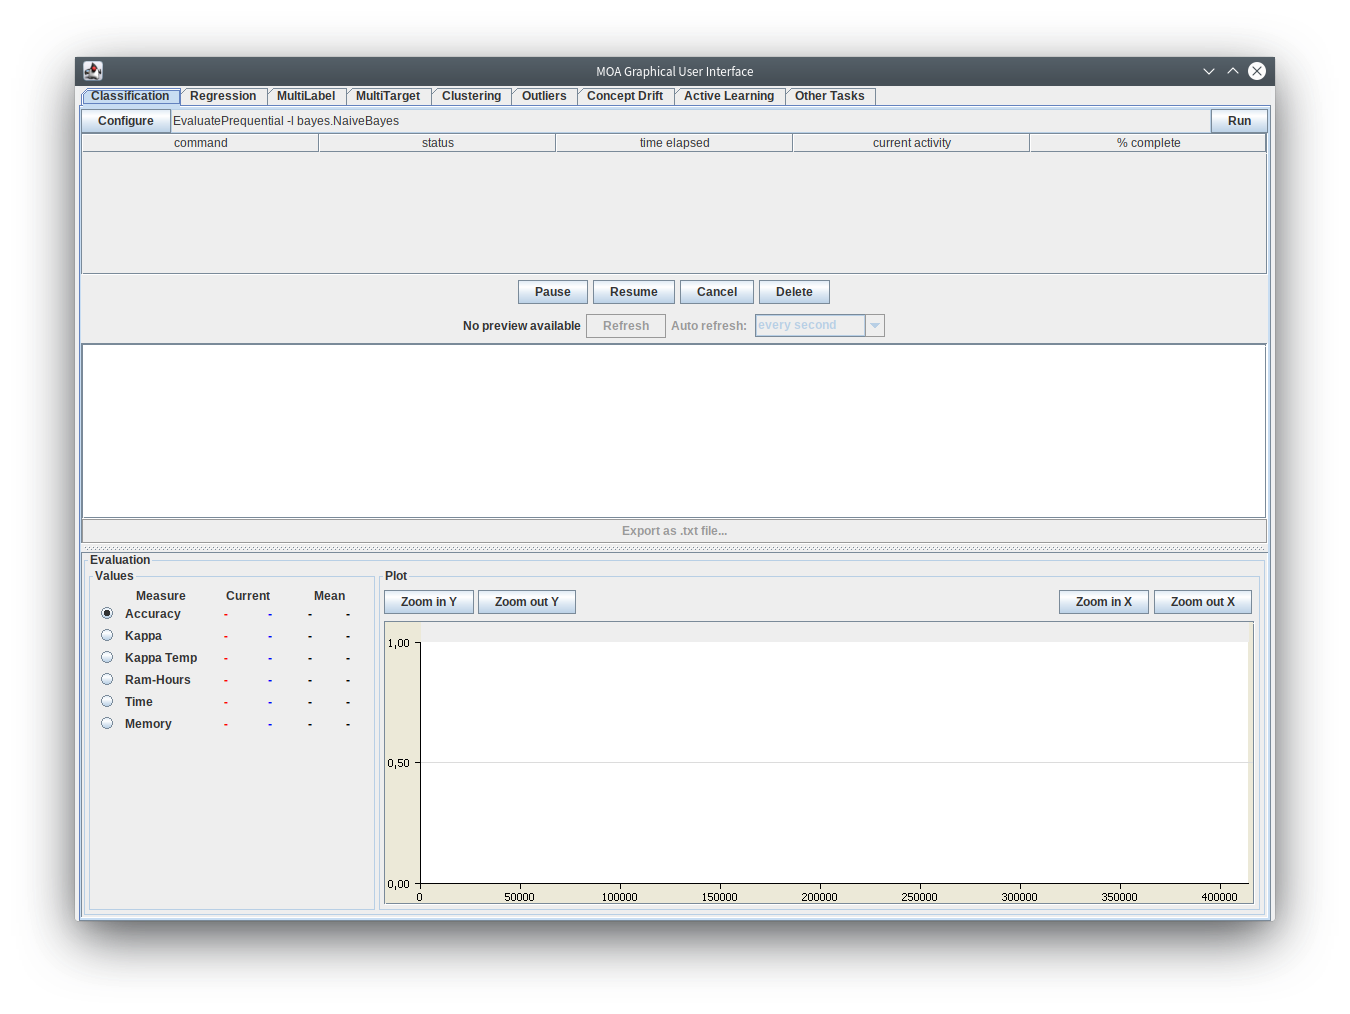
\includegraphics[scale=0.4]{imagens/moa.png}
    \caption{MOA - Tela Inicial}
    \label{fig:moa}
\end{center}
\end{figure}

A aplicação é capaz de ler arquivos em formato ARFF\footnote{\textit{Attribute-Relation File Format}}, além de permitir a produção de fluxos de dados dinamicamente, através de geradores.
Alguns dos geradores de fluxo disponíveis no MOA são:
\textit{Random Trees} \cite{Domingos:2000:MHD:347090.347107}
\textit{SEA} \cite{Street:2001:SEA:502512.502568},
\textit{STAGGER} \cite{Schlimmer1986},
\textit{Rotating Hyperplane} \cite{Wang:2003:MCD:956750.956778},
\textit{Random RBF},
\textit{LED} \cite{Gama:2003:ADT:956750.956813},
\textit{Waveform} \cite{Gama:2003:ADT:956750.956813},
 e \textit{Function} \cite{Jin:2003:EDT:956750.956821}.

Outra funcionalidade importante do framework é a possibilidade de adicionar mudanças de conceito a fluxos estacionários existentes.
Esse processo é realizado através de uma função sigmóide, que modela o evento de mudança de conceito como uma combinação balanceada de duas distribuições homogêneas,
que caracterizam os conceitos-alvo antes e depois da mudança.
Além destes conceitos, o usuário também pode definir o momento da mudança e a sua duração \cite{Bifet:2010:MMO:1756006.1859903}.

A arquitetura do framework é modular, o que permite a implementação de novos algoritmos de forma trivial.
Por exemplo, para incluir um novo algoritmo de detecção de mudanças de conceito, basta estender a classe abstrata \textit{AbstractChangeDetector} e implementar o algoritmo desejado.
A janela de configuração deste detector, similar a Figura \ref{fig:moa_detector}, será criada dinamicamente, a partir dos atributos definidos na classe.

\begin{figure}[H]
\begin{center}
    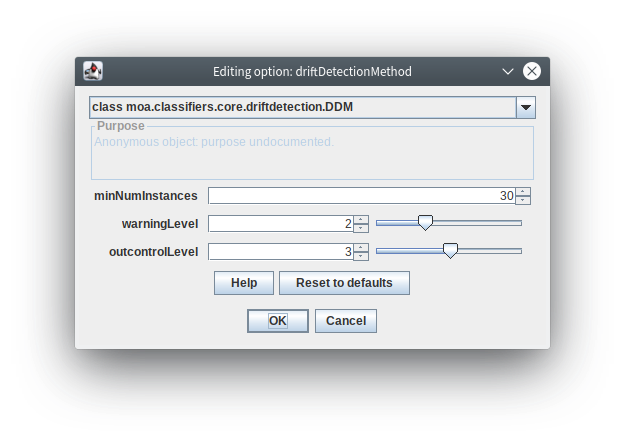
\includegraphics[scale=1]{imagens/detector.png}
    \caption{MOA - Configuração detector}
    \label{fig:moa_detector}
\end{center}
\end{figure}

Os principais algoritmos para detecção de mudanças de conceito possuem implementação disponível no MOA.
Além dessas implementações, a ferramenta também disponibiliza rotinas de avaliação, que analisam a acurácia e o desempenho desses métodos.

Esta dissertação utilizou o MOA como plataforma para realização do experimento com dados sintéticos.
Os conjuntos de dados usados foram gerados através da ferramenta e o método proposto foi implementado e comparado aos principais algoritmos disponíveis. 
Por fim, os testes realizados foram avaliados através da classe \textit{BasicConceptDriftPerformanceEvaluator}.

\section{Redes de Função de Base Radial}
\label{sec:rbf}

Uma Rede de Função de Base Radial (redes RBF, em português,  ou \textit{radial basis function network, RBF network}, em inglês) pode ser definida como um modelo de múltiplas camadas alimentadas adiante (\textit{feedforward}),
capaz de analisar padrões complexos e resolver problemas não-linearmente separáveis, utilizando uma abordagem de aproximação de funções.
Estas redes têm como principal diferencial a sua forma de ativação, realizada através do cálculo da distância entre o dado e um centro definido \cite{Braga:RedesNeuraisTeoriaAplicacoes}.

A arquitetura de uma rede de função de base radial, em sua forma mais básica, envolve três camadas.
A camada de entrada representa os atributos do problema. As unidades dessa camada não realizam processamento e simplesmente distribuem as entradas para a camada intermediária.
A camada intermediária, única camada oculta da rede, é constituída por funções de ativação de base radial, que atuam como os neurônios da rede.
Por fim, a camada de saída pondera, através de pesos, os resultados da camada intermediária, agregando-os linearmente para compor a resposta final da rede \cite{Rojas:1996:NNS:235222}.
A Figura \ref{fig:rbg_arq} demonstra essa arquitetura.

Na literatura, as funções Gaussianas (Função \ref{eq:gaussiana}) são as funções de ativação mais usuais em redes RBF, sendo definidas por seus centros e larguras:

\begin{equation}
    \label{eq:gaussiana}
    \varphi (v_{i})=e^{-(\sigma r)^{2}}
\end{equation}

onde, $r$ é a distância euclidiana ($\|\mathbf {v_{i}} - \mathbf {c_{i}}\|$), $v$ é o valor de entrada, $c_i$ representa o centro e $\sigma$ é o parâmetro limitador do raio.

\begin{figure}[H]
\begin{center}
    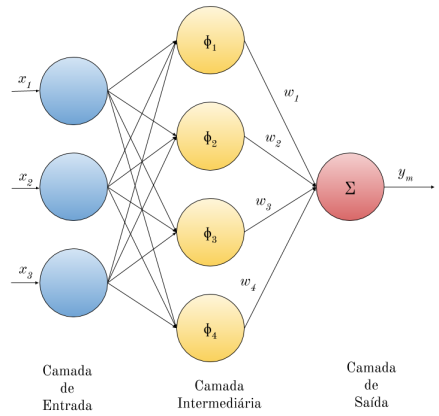
\includegraphics[scale=1]{imagens/rbf_arq.png}
    \caption{Arquitetura RBF}
    \label{fig:rbg_arq}
\end{center}
\end{figure}

A modelagem das redes RBF define a entrada como um vetor de números reais ${x} \in {R} ^{n}$ e o resultado da rede como uma função escalar desse vetor $\varphi : {R} ^{n} \to {R}$.
Esta função é obtida a partir da combinação linear dos resultados das funções de ativação (Equação \ref{eq:rbf1}).

\begin{equation} \label{eq:rbf1}
    \varphi ({x})=\sum _{{i=1}}^{N}a_{i}\rho (||{x}-{c}_{i}||)
\end{equation}

onde $N$ é o número de neurônios na camada intermediária, ${c}_{i}$ é o centro do neurônio $i$, $||\ldots||$ é a norma euclidiana e $a_{i}$ é o peso (bias) atribuído ao neurônio para realização da combinação linear.

O método de detecção proposto nesta dissertação utiliza uma rede RBF adaptada, composta apenas pelas camadas inicial e intermediária.
Esta adaptação é possível, pois o processo de ativação realizado na camada intermediária produz, implicitamente, grupos a partir das observações recebidas ao longo do tempo.
Possíveis mudanças de conceito são, então, identificadas quando o grupo ativo deste agrupamento é alterado.

\section{Cadeias de Markov}
\label{sec:markov}

Equações determinísticas são utilizadas para descrever sistemas cuja evolução pode ser traçada a partir de uma condição inicial.
Entretanto, isto nem sempre é viável, pois alguns sistemas apresentam diferentes possibilidades evolutivas.
Nestes casos, processos estocásticos são utilizados \cite{taylor1998introduction}.

Um processo estocástico, $\left\{ X _ { t } : t \in T \right\}$, é uma coleção de variáveis aleatórias indexadas no tempo.
O conjunto de possíveis valores, $X_{t}, S = \left\{s_{1}, s_{2}, \ldots\right\}$, é denominado espaço dos estados e $T$ denota o espaço temporal.
A partir desta definição e considerando que o processo estocástico esteja no estado $s_i$ e no tempo $t - 1$, a probabilidade
do processo estar no estado $s_j$ no tempo $t$ é dada pela Equação \ref{eq:prob_proc_estoc}:

\begin{equation}
    \label{eq:prob_proc_estoc}
    \mathbb { P } \left( X _ { t } = s _ { j } | X _ { t - 1 } = s _ { i } , \ldots , X _ { 0 } = s _ { 0 } \right)
\end{equation}

% A probabilidade resultante desta equação é denominada probabilidade de transição (de um passo) do estado $s_i$ para o estado $s_j$.

Uma Cadeia de Markov, ou Processo de Markov,
é um processo estocástico no qual a probabilidade de um sistema estar em determinado estado em um dado período de tempo depende apenas do estado no período imediatamente anterior.
Esse tipo de processo também é conhecido como processo sem memória (\textit{memoryless process}, em inglês), pois os estados passados são ignorados.
Esta característica é demonstrada através da Equação \ref{eq:markov}:

\begin{equation}
    \label{eq:markov}
    \mathbb { P } \left( X _ { t } = s _ { j } | X _ { t - 1 } = s _ { i } , \ldots , X _ { 0 } = s _ { 0 } \right) = \mathbb { P } \left( X _ { t } = s _ { j } | X _ { t - 1 } = s _ { i } \right) = p _ { i j }
\end{equation}

Ou seja, um processo de Markov pode assumir os estados $a_1, a_2, \ldots, a_r$, de tal modo que a probabilidade
de transição de um estado $a_i$ para um estado $a_j$ seja $P_{ij}$ (um valor dependente apenas de $i$ e $j$).
Portanto, é viável elaborar uma matriz com as probabilidades de todas transições.
Esta matriz é denominada matriz estocástica e um exemplo é apresentado na Equação \ref{eq:matriz_estocastica}:

\begin{equation}
\label{eq:matriz_estocastica}
P = \left[ \begin{array} { c c c c } { P _ { 11 } } & { P _ { 12 } } & { \dots } & { P _ { 1 r } } \\ { P _ { 21 } } & { P _ { 22 } } & { \dots } & { P _ { 2 r } } \\ { \vdots } & { \vdots } & { \vdots } & { \vdots } \\ { P _ { r 1 } } & { P _ { r 2 } } & { \cdots } & { P _ { r r } } \end{array} \right]
\end{equation}

A fim de ilustrar os conceitos apresentados, considere o diagrama de estados representado na Figura \ref{fig:cadeia_markov_tres_estados}.
Este diagrama detalha um processo Markoviano com três estados possíveis, em um determinado instante de tempo:



\begin{figure}[H]
    \begin{center}
        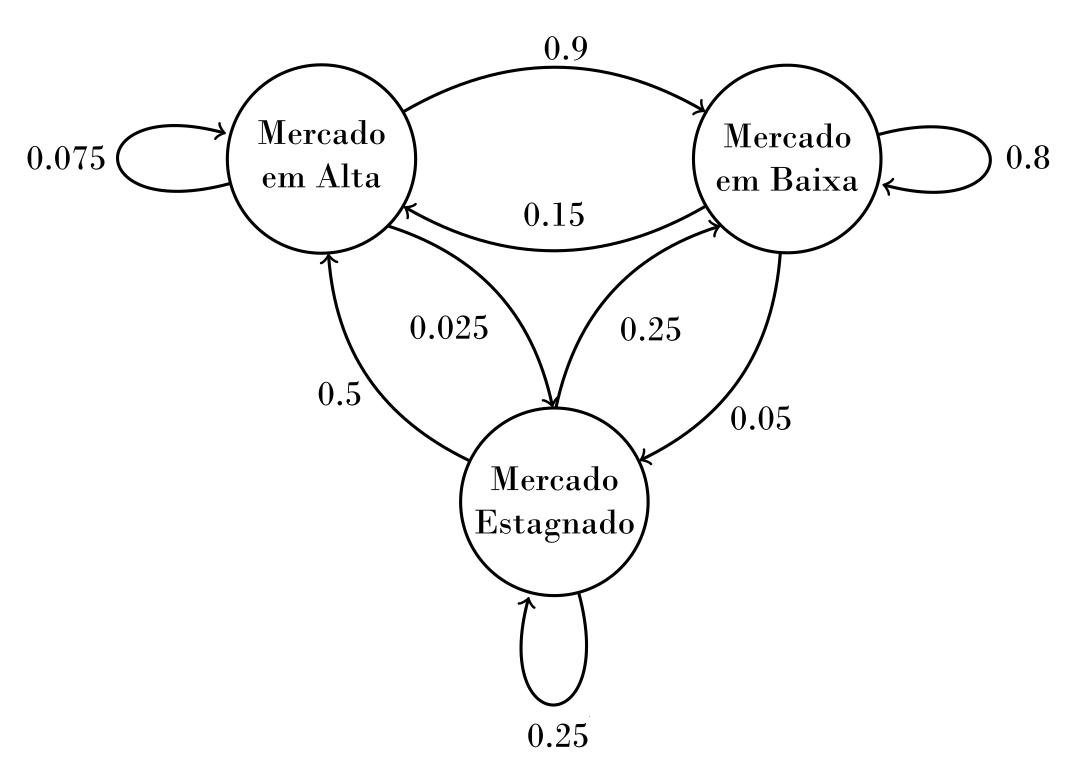
\includegraphics[scale=0.35]{imagens/markov_chain_wikipedia.png}
        \caption{Exemplo: Cadeia de Markov com três estados.}
        \label{fig:cadeia_markov_tres_estados}
    \end{center}
\end{figure}

Este diagrama também pode ser representado como uma matriz estocástica, demonstrada na Equação \ref{eq:matriz_estocastica_exemplo}.

\begin{equation}
\label{eq:matriz_estocastica_exemplo}
P={\begin{bmatrix}0.9&0.075&0.025\\0.15&0.8&0.05\\0.25&0.25&0.5\end{bmatrix}}.
\end{equation}

O algoritmo de detecção de mudanças de conceito proposto nesta dissertação utiliza uma Cadeia de Markov para modelar o agrupamento criado na rede RBF. Os grupos formados representam os estados do modelo markoviano e as mudanças (ativações) entre estes grupos, as transições.
Estas mudanças são refletidas no modelo através do aumento da probabilidade  correspondente e a diminuição proporcional das outras transições. Estas alterações são realizadas respeitando a condição $0 \leq P_{ij} \leq 1$.


\section{Trabalhos Relacionados}
\label{sec:trabalhos_relacionados}

Durante a elaboração desta dissertação, foi realizada uma pesquisa na literatura em busca de trabalhos que propusessem métodos para identificação de mudanças de conceito, de forma online e independente de rótulos, em fluxos contínuos de dados. Também foram estudadas técnicas que pudessem subsidiar o desenvolvimento de novos algoritmos que atendam a esses requisitos.

Inicialmente, foram analisados os algoritmos \textit{Implícitos / Não Supervisionados} pertencentes a subcategoria \textit{Detecção de Novidade / Métodos de Agrupamento}. Estes algoritmos são descritos a seguir.

O algoritmo \textit{OnLIne Novelty and Drift Detection Algorithm} (OLINDDA) utiliza a técnica de agrupamento \textit{K-means} para monitorar e se adaptar ao surgimento de novos padrões \cite{Spinosa:2007:OCA:1244002.1244107}.
Os exemplos recepcionados são incluídos em uma fila e são periodicamente agrupados. Os grupos resultantes desse processamento definem se os exemplos devem ser incorporados a um grupo existente ou formar um novo grupo.

O algoritmo MINAS, proposto por \citeonline{Faria:2013:NDA:2480362.2480515}, atua de forma similar ao algoritmo OLLINDA, contudo utiliza \textit{micro clusters} obtidos a partir da aplicação de uma técnica de agrupamento específica para fluxos contínuos de dados (CluStream) e estende a abordagem para permitir a aplicação em problemas multiclasse.

O algoritmo DETECTNOD \cite{Hashemi:Hayat:DETECTNOD:2010} utiliza um modelo de clusterização para delimitar os exemplos observados.
Uma representação compacta desses grupos é produzida através da Transformada Discreta de Cosseno. Esta representação é utilizada, em conjunto com o algoritmo de vizinho mais próximo, para aproximar novos exemplos.
Estes exemplos são categorizados como desvios ou novidades, conforme o grau de similaridade calculado.

Os algoritmos Woo \cite{Lee:Wang:Ryu:2007} e ECSMiner \cite{Masud:2011:CNC:1978259.1978529} também se baseiam no conceito de \textit{micro clusters}. A técnica Woo atribui um classificador para cada cluster formado. Estes classificadores são utilizados para verificar a similaridade de novos exemplos em relação ao cluster. Exemplos que não se enquadram em nenhum grupo são marcados como suspeitos e passam a ter sua densidade monitorada. Um número crescente de vizinhos no raio dos exemplos monitorados indica o surgimento de um novo conceito, induzindo o retreino do modelo e ajuste do centróide do agrupamento.
O ECSMiner \cite{Masud:2011:CNC:1978259.1978529} utiliza o conceito de Outliers Filtrados, que se refere a amostras que estão fora do limite de todos os clusters existentes, em uma abordagem similiar ao algoritmo Woo.

O algoritmo GC3 \cite{Sethi2016b:GC3} estende a ideia de \textit{micro clusters} ao aplicar um algoritmo de agrupamento baseado em grade e densidade. Dessa forma, novos padrões são identificados a partir do surgimento de novas áreas de alta densidade.

Os algoritmos baseados em técnicas de detecção de novidade utilizam métodos de agrupamento para identificar padrões emergentes. Portanto, também apresentam dificuldade para lidar com alta dimensionalidade e/ou dados binários, por dependerem do cálculo de distância, e são computacionalmente custosos.

A segunda etapa da pesquisa analisou técnicas para detecção de mudanças de conceito em séries temporais que atuam de forma online. Estas técnicas também são comumente denominadas como técnicas para detecção de \textit{change points}. A maioria dos trabalhos identificados se baseia no monitoramento dos valores residuais da aplicação de um modelo. Nesta abordagem, um modelo estatístico ou de Aprendizado de Máquina é aplicado a um conjunto de observações extraídas da série temporal, representando um conceito.
Assume-se que se não houver mudança de conceito, os valores residuais dessa aplicação devem ser estacionários. Os trabalhos identificados são apresentados a seguir.

\citeonline{Yamanishi:2002:UFD:775047.775148} propõem um método de detecção online capaz de identificar outliers e mudanças de conceito em séries temporais.
A abordagem aplica um modelo autoregressivo aos dados e atualiza os parâmetros de forma incremental, para que o peso de exemplos passados diminua ao longo do tempo. Atribui-se uma pontuação para cada observação, calculada com base na função de perda. Esta pontuação indica o grau de desvio do dado em relação ao modelo aplicado. Pontuações elevadas indicam alta possibilidade de que o dado seja um outlier. A detecção de mudanças de conceito é feita através do monitoramento da média das funções de perda ao longo da série temporal. Todavia, esta abordagem só é aplicável a séries temporais com comportamento autoregressivo, o que limita o seu escopo de uso.

\citeonline{GOMBAY2009715} propõem um método diferente, também online, para detecção de mudanças em séries temporais autoregressivas, baseado no monitoramento dos parâmetros do modelo. Um adaptação do método CUSUM \cite{Page:CUSUM:PageHinkley:1954} é aplicada para identificar alterações nos parâmetros. A hipótese nula do algoritmo assume que estes parâmetros devem permanecer estacionários ao longo do tempo. Esta hipótese é testada para cada nova observação recepcionada e a mudança de conceito é sinalizada quando a diferença ultrapassa um limite estabelecido. Esta abordagem também apresenta limitação de escopo, pois é aplicável apenas a séries temporais autoregressivas.

A utilização de valores residuais para detecção de mudanças de conceito  apresenta desvantagens. Por serem baseados na acurácia do modelo aplicado, estes métodos sofrem influência de problemas ocorridos durante a parametrização ou fase de treinamento. Em teoria, o monitoramento direto de características dos dados pode permitir uma identificação de mudanças de conceito mais robusta.

Poucos estudos utilizam as características das séries temporais para identificar mudanças de conceito. Neste contexto, o trabalho proposto por  \citeonline{Boracchi2014ExploitingSF} se destaca por apresentar um método de detecção de mudanças de conceito em séries temporais que atua de forma online, baseando-se no monitoramento da característica de auto-similaridade da série.
Entretanto, o método proposto tem como principal limitação o fato de ser especializado para séries que apresentam auto-similaridade e periodicidade. Além disso, a abordagem utiliza uma considerável quantidade de memória, pois armazena uma sequência de dados que representa o comportamento estável ou regular da série temporal.

Para cenários nos quais os fluxos de dados não apresentam as propriedades esperadas pelas técnicas discutidas anteriormente, \citeonline{StableApproachToDetectConceptDrift:Mello} propõem um novo método para detecção de mudanças de conceito que atua de forma online.
Este trabalho se diferencia por utilizar um algoritmo de agrupamento hierárquico estável, conforme a propriedade proposta por \citeonline{Carlsson:2010:CSC:1756006.1859898}.
A abordagem cria janelas consecutivas de dados. A técnica de agrupamento é aplicada em cada janela e os dendogramas resultantes comparados, a fim de identificar mudanças de conceito na distribuição dos dados.

As técnicas para detecção de mudanças de conceito são, geralmente, aplicadas para minimizar o intervalo entre a ocorrência da mudança e a atualização do modelo aplicado. Diante disso, um método de detecção ideal deve:

\begin{itemize}
    \item ser transparente para o usuário, detectando e informando explicitamente sobre a ocorrência de mudanças;
    \item ser computacionalmente eficiente;
    \item atuar de forma online, buscando minimizar o atraso de atualização do modelo; e
    \item basear-se em características dos dados que reflitam os conceitos presentes.
\end{itemize}

Por fim, a pesquisa realizada evidenciou a inexistência de técnicas que atendam a todos esses requisitos e que sejam computacionalmente eficientes,
independentes de rótulos e aplicáveis a fluxos de dados de qualquer natureza.
Esta dissertação de mestrado tem como objetivo preencher esta lacuna,
através da proposição de um novo método, baseado em Redes de Função de Base Radial e Cadeias de Markov,
para identificação de mudanças de conceito em fluxos contínuos de dados.

\section{Considerações Finais}

Neste capítulo foram apresentados os conceitos que fundamentaram esta dissertação: Fluxos de Dados, Mudanças de Conceito, Redes de Função de Base Radial e as Cadeias de Markov.
Por fim, os trabalhos relacionados identificados na literatura foram discutidos.

\xchapter{RBFC\element{hain}}{} \label{rbfchain}

\section{Considerações Iniciais}

Este capítulo descreve o método para detecção de mudanças de conceito proposto por esta dissertação, denominado RBFChain.
O método proposto é descrito da seguinte forma:
a Seção \ref{sec:rbfchain_visao_geral} apresenta uma visão geral da solução, demonstrando a arquitetura, o ciclo de execução e a função desempenhada por cada componente.
Em seguida, na Seção \ref{sec:rbfchain_detalhes}, o algoritmo desenvolvido é apresentado na forma de pseudocódigo e o seu comportamento é detalhado através de uma execução de exemplo.
Por fim, na Seção \ref{sec:rbfchain_consideracoes_finais}, são emitidas as considerações finais do capítulo.

\section{Visão Geral}
\label{sec:rbfchain_visao_geral}

O RBFChain atua diretamente sobre o fluxo de dados e é composto por dois componentes principais: uma Rede de Função de Base Radial (RBF) adaptada e uma Cadeia de Markov.
A arquitetura da solução é demonstrada na Figura \ref{fig:arquitetura}. 

\begin{figure}[H]
    \begin{center}
        
\includegraphics[scale=0.6]{imagens/arquitetura_rbfchain.png}
        \caption{Arquitetura RBFChain}
        \label{fig:arquitetura}
    \end{center}
\end{figure}

O restante desta seção apresenta, resumidamente, o ciclo de execução e a função desempenhada por cada componente:

\begin{enumerate}
    \item O ciclo de execução se inicia quando um novo evento é observado a partir do fluxo de dados;
    
    \item O evento é, então, encaminhado para rede RBF, que produz grupos das observações recebidas, representando os \textit{conceitos} do sistema.
    Durante este processo, o evento pode ser vinculado ao mesmo \textit{conceito} que o evento anterior ou a um novo \textit{conceito}. 
    A manutenção ou mudança do \textit{conceito} vinculado caracteriza uma \textit{transição};
    
    \item Em seguida, a Cadeia de Markov atualiza a probabilidade da \textit{transição} ocorrida;
    
    \item Logo após, a probabilidade resultante é informada ao RBFChain;
    
    \item Por fim, o RBFChain verifica se o \textit{conceito} mudou e compara a probabilidade da \textit{transição} ao valor mínimo para detecção de mudanças de conceito. Se for inferior, emite um sinal de \textit{zona de alerta}. Do contrário, indica a ocorrência de uma \textit{mudança de conceito}.
\end{enumerate}

\section{Algoritmo}
\label{sec:rbfchain_detalhes}

Esta seção apresenta o método proposto na forma de pseudocódigo\footnote{Implementações do algoritmo na linguagem Python e Java estão disponíveis, respectivamente, em: \url{https://github.com/rnetodev/masters/tree/master/experiments} e \url{https://github.com/rnetodev/moa}} em Algoritmo \ref{alg:algoritmo} e descreve o seu funcionamento. 
Logo depois, uma execução de exemplo é detalhada.

\vspace{7pt}
\begin{algorithm}[H]
    \SetAlgoLined
    \Entrada{$evento, \sigma, \lambda, \alpha, \delta$}
    \Saida{$nulo, alerta$ ou $mudanca$}
    \Inicio{

     $grupos \longleftarrow ()$\; 
     $grupoAtivo \longleftarrow nulo$\; 
     $grupoConceito \longleftarrow nulo$\;
     $retorno \longleftarrow nulo$\;
     
     \BlankLine
     
     $minAtivacao \longleftarrow \lambda$\;
     \ParaTodo{grupo}{
         $ativacao \longleftarrow gaussiana(evento, grupo, \sigma)$\\
         \Se{$ativacao >= minAtivacao$}{
            $grupoAtivo \longleftarrow grupo$\;
            $minAtivacao \longleftarrow ativacao$\;
         }
    }
    \Se{$grupoAtivo == nulo$}{
        $grupos \longleftarrow evento$\;
        $grupoAtivo \longleftarrow evento$\;
    }
    
    \BlankLine
    
    \Se{$grupoConceito == nulo$}{
        $grupoConceito \longleftarrow grupoAtivo$\;
    }
    
    \BlankLine
         
    $probabilidade \longleftarrow markov(grupoConceito, grupoAtivo, \alpha)$\;

    \BlankLine
    
    \Se{$grupoConceito \neq grupoAtivo$}{
        \Se{$probabilidade < \delta$}{
            $retorno \longleftarrow alerta$\;
        }
        \Senao{
            $grupoConceito \longleftarrow grupoAtivo$\;
            $retorno \longleftarrow mudanca$\;
        }
    }
    
    \BlankLine

    \Retorna{$retorno$}\;
    }

    \caption{\textsc{RBFChain}}
    \label{alg:algoritmo}
\end{algorithm}
\vspace{7pt}

\newpage

\subsection{Descrição do algoritmo}

Para descrever o funcionamento do algoritmo, é necessário apresentar os quatro parâmetros de configuração requeridos. Destes, dois são relacionados à Rede de Função de Base Radial e dois à Cadeia de Markov:

\begin{itemize}
    \item \textbf{Parâmetros relacionados à Rede de Função de Base Radial}:
    \begin{itemize}
        \item \textbf{$\sigma$}: limita o raio da função Gaussiana,  utilizada durante o processo de ativação;
        \item \textbf{$\lambda$}: valor mínimo para ativação de um grupo.
    \end{itemize}

    \item \textbf{Parâmetros relacionados à Cadeia de Markov}:
    \begin{itemize}
        \item \textbf{$\alpha$}: valor de incremento para as transições ocorridas;
        \item \textbf{$\delta$}: probabilidade mínima para identificação de uma mudança de conceito.
    \end{itemize}
\end{itemize}

A execução do algoritmo começa quando um novo evento é observado a partir do fluxo de dados. O evento é, então, submetido ao processo de ativação da rede RBF (linhas 6 a 14), que produz grupos das observações recebidas, representando os \textit{conceitos} do sistema. 

Para execução do agrupamento, é necessário calcular o valor de ativação do evento para cada grupo, através da função Gaussiana (linha 8). 
Como resultado, o grupo com maior valor de ativação é definido como \textit{grupo ativo}. Se nenhum grupo alcançar o valor mínimo de ativação ($\lambda$) (linha 12), define-se o próprio evento como um novo \textit{grupo ativo} (linhas 13 a 14). 

Em seguida, o algoritmo verifica se o \textit{grupo conceito} (grupo que representa o conceito vigente) está definido. Se não estiver, define o \textit{grupo ativo} como \textit{grupo conceito} (linhas 15 e 16). Este passo ocorre durante a formação do primeiro grupo.

Logo após, o RBFChain persiste na Cadeia de Markov a transição entre o \textit{grupo conceito} e o \textit{grupo ativo} (linha 17). 
O procedimento de persistência incrementa a probabilidade da transição ocorrida pelo fator $\alpha$ e reduz proporcionalmente a probabilidade das outras transições.

Por fim, o algoritmo verifica se o \textit{grupo conceito} é diferente do \textit{grupo ativo} (linhas 18 a 23).
Se esta condição for verdadeira e a probabilidade da transição for inferior a $\delta$, emite o sinal de \textit{zona de alerta}. 
Entretanto, se a probabilidade for superior, o \textit{grupo ativo} é definido como novo \textit{grupo conceito} e uma mudança de conceito é sinalizada.

\subsection{Execução de exemplo}

Esta subseção apresenta uma execução de exemplo do RBFChain, visando elucidar o seu funcionamento.
Para este exemplo, o conjunto $S$ foi utilizado como fonte de dados e os parâmetros definidos de forma empírica:

\[
S = \{0.11, 0.12, 0.13, 0.33, 0.34, 0.45, 0.6, 0.33, 0.25, 0.14, 0.11, 0.15\}
\]
\[
\sigma = 3, \lambda = 0.8, \alpha = 0.25, \delta = 0.5
\]

O comportamento do algoritmo durante a análise do conjunto $S$ é descrito a seguir.

No instante $T1$ o evento $0.11$ é observado.
Por não existir nenhum outro grupo, o evento é definido como \textit{grupo ativo} e \textit{grupo conceito}, e a transição $0.11 \rightarrow 0.11$ (\textit{grupo conceito} $\rightarrow$ \textit{grupo ativo}) persistida no modelo markoviano.

Em $T2$ e $T3$ são recebidos, respectivamente, os valores $0.12$ e $0.13$, que são vinculados ao grupo $0.11$, pois seus valores de ativação são maiores que $0.8$ ($\lambda$). 
O \textit{grupo conceito} permanece inalterado, logo a transição $0.11 \rightarrow 0.11$ é persistida duas vezes.

No instante $T4$ o evento $0.33$ é recebido, mas não atinge o valor mínimo de ativação (\textit{$\lambda$}) para os grupos existentes ($\{0.11\}$).
Dessa forma, o evento é definido como novo \textit{grupo ativo} e a probabilidade da transição $0.11 \longrightarrow 0.33$ é atualizada. 
O \textit{grupo ativo} ($0.33$) é diferente do \textit{grupo conceito} ($0.11$), mas a probabilidade da transição ainda é inferior a $\delta$, portanto apenas o sinal de zona de alerta é emitido e o \textit{grupo conceito} permanece como $0.11$.

No momento $T5$ o evento $0.34$ é recepcionado e vinculado ao grupo $0.33$, ativando-o.
A transição do \textit{grupo conceito} para o \textit{grupo ativo} ($0.11 \rightarrow 0.33$) é persistida e a probabilidade da transição passa a ser maior que $\delta$, ocasionando uma mudança de conceito. O \textit{grupo conceito} passa, então, a ser $0.33$.
Logo depois, no instante $T6$, o valor $0.45$ é observado e vinculado ao grupo $0.33$, persistindo a transição $0.33 \rightarrow 0.33$, pois o \textit{grupo conceito} foi alterado no instante anterior.

Em $T7$, um \textit{outlier} de valor $0.6$ é observado, constituindo um novo \textit{grupo ativo}. A transição persistida ($0.33 \rightarrow 0.6$) tem valor inferior a $\delta$, portanto, apenas um sinal de zona de alerta é emitido.
Este evento denota a tolerância a ruídos do método proposto, devido a modelagem na Cadeia de Markov.

Em seguida, nos instantes $T8$ e $T9$, os eventos $0.33$ e $0.25$ são recebidos e vinculados ao grupo $0.33$. 
Por fim, nos instantes $T10$, $T11$ e $T12$, ocorre uma nova mudança de conceito, tornando o grupo $0.11$ novamente o \textit{grupo conceito}.

A Figura \ref{fig:funcionamento_algoritmo} apresenta o comportamento do algoritmo durante a análise do conjunto de dados. As cores dos círculos diferenciam o \textit{grupo ativo} de cada evento, as linhas sólidas na cor cinza demonstram os sinais de zona de alerta e as linhas sólidas na cor vermelha representam as mudanças de conceito. As seguintes abreviações também foram utilizadas: \textbf{E}, indicando o evento observado; \textbf{GA}, representando o \textit{grupo ativo} para o evento; e, \textbf{GC}, identificando o \textit{grupo conceito} definido após a análise do evento.

De forma complementar, a Figura \ref{fig:evolucao_markov} evidencia a evolução do modelo markoviano ao longo da execução de exemplo. Na imagem, os estados na cor cinza representam o \textit{grupo conceito} no instante de tempo.

\begin{landscape}
    \begin{figure}[ht]
    \begin{center}
        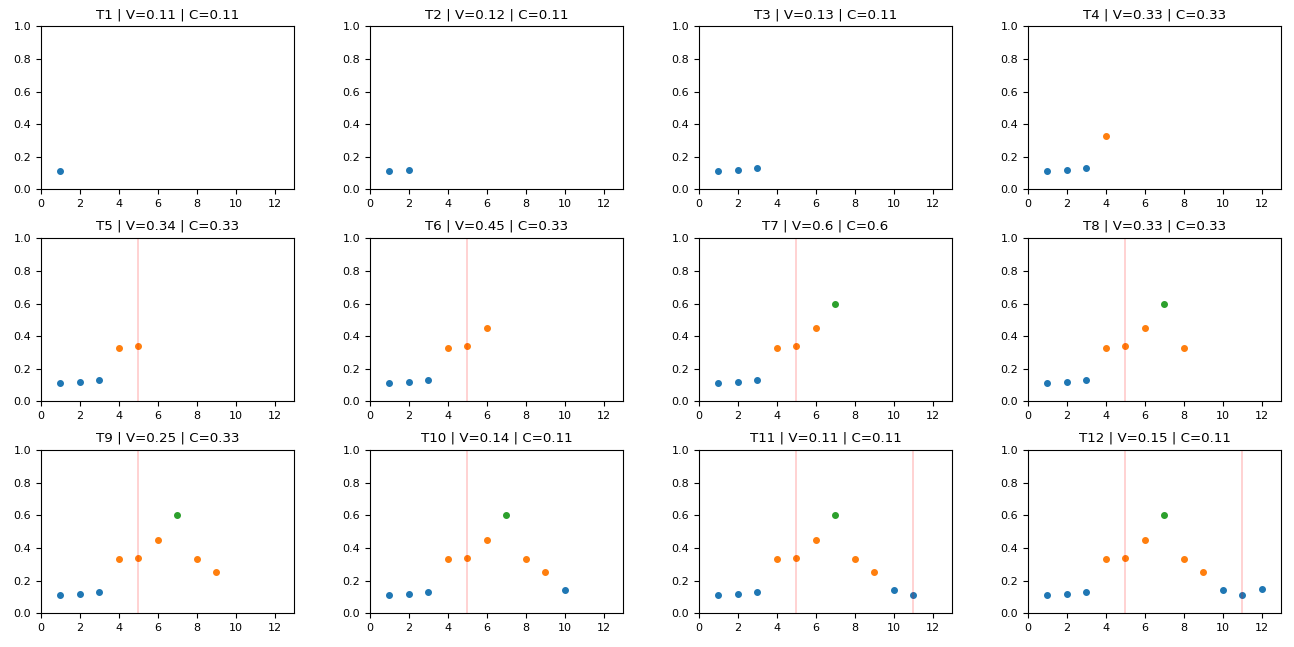
\includegraphics[scale=0.7]{imagens/funcionamento_algoritmo.png}
        \caption{Execução de exemplo do RBFChain}
        \label{fig:funcionamento_algoritmo}
    \end{center}
    \end{figure}
\end{landscape}

\begin{landscape}
\begin{figure}[ht]
    \begin{center}
        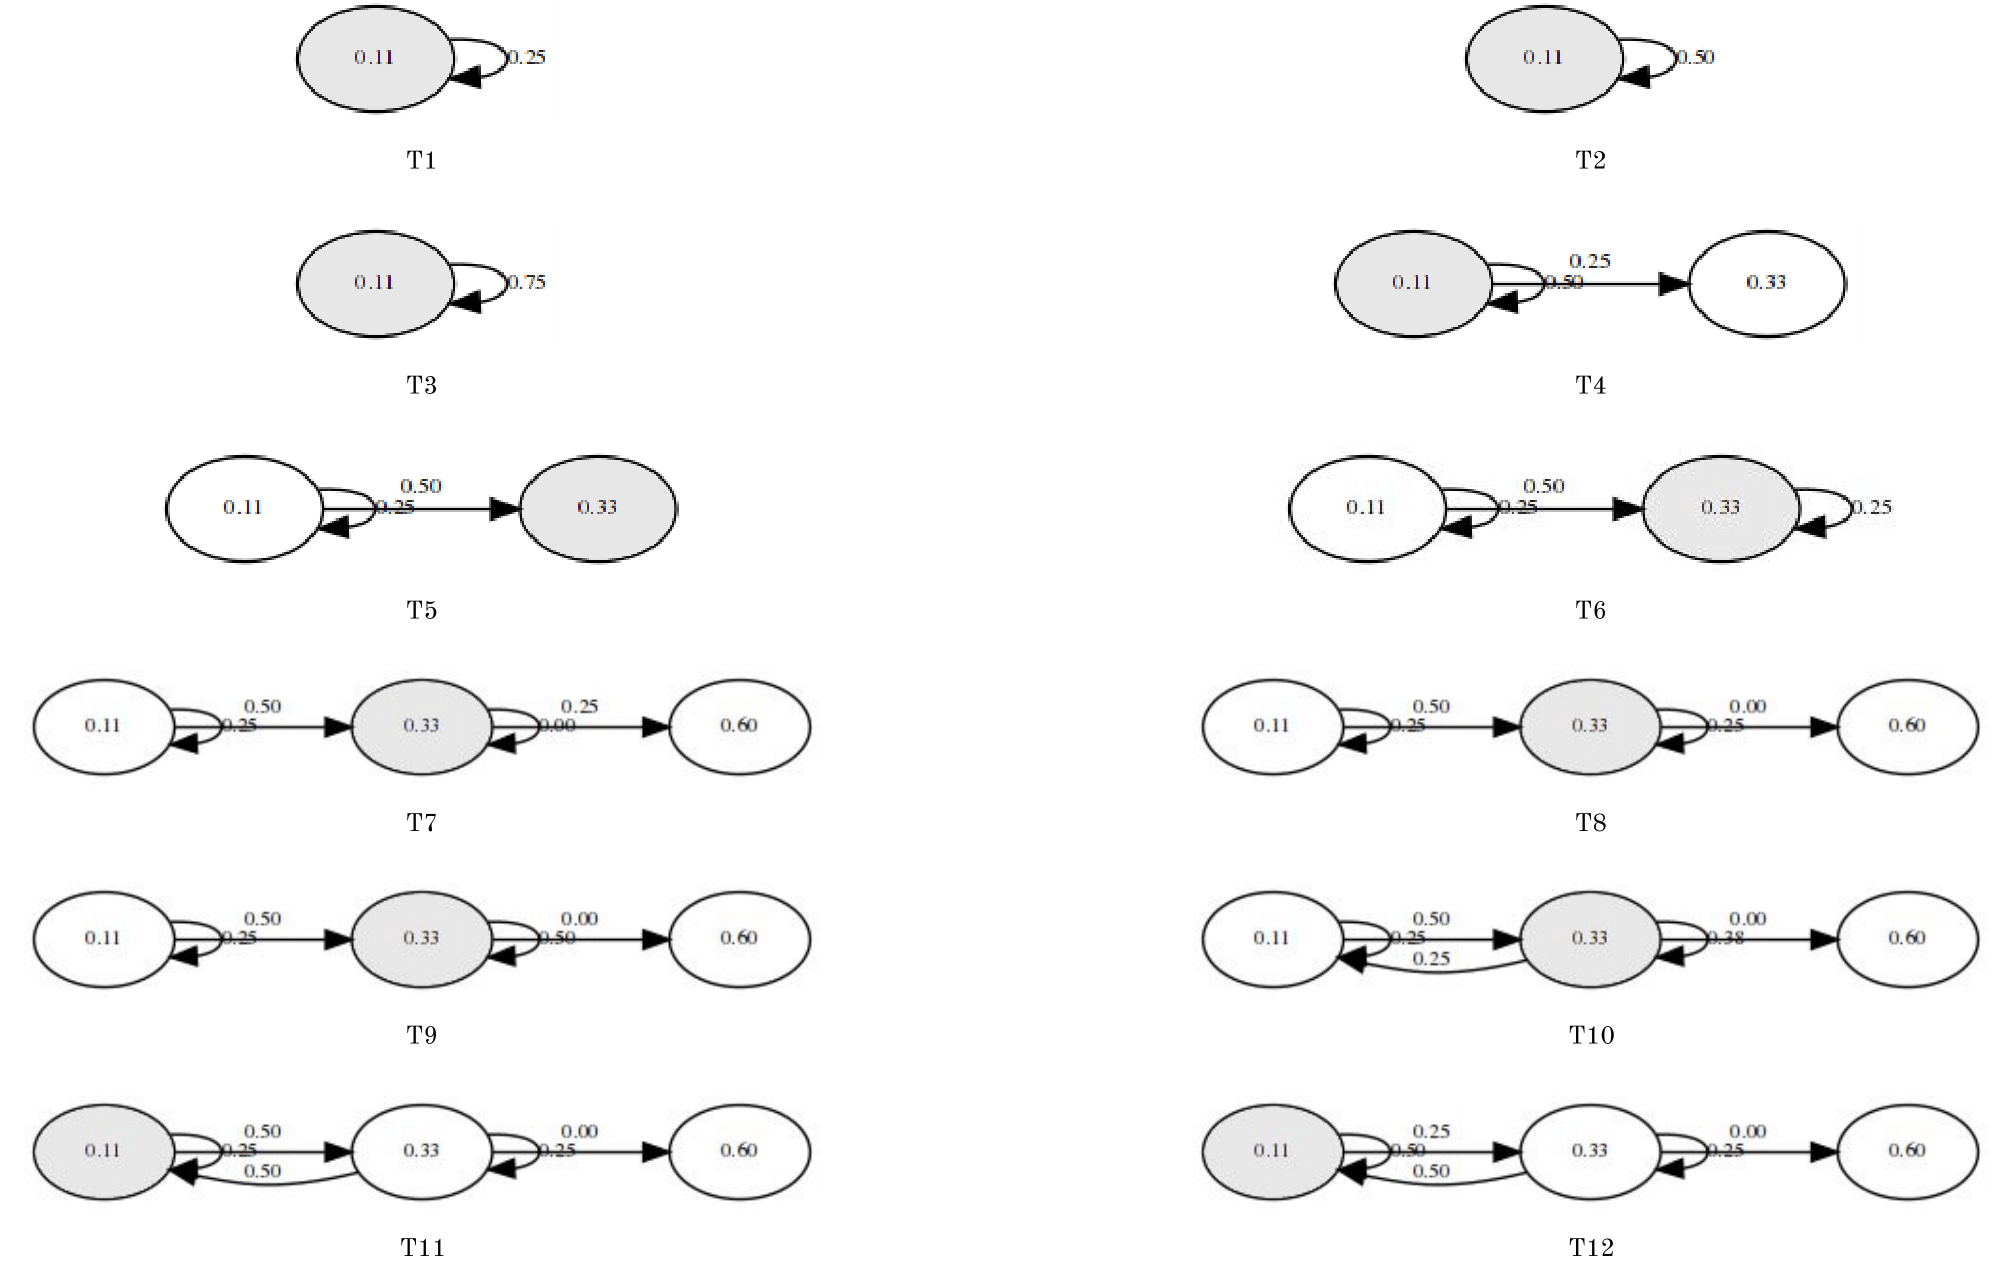
\includegraphics[scale=0.4]{imagens/evolucao_markov.png}
        \caption{Evolução do modelo markoviano}
        \label{fig:evolucao_markov}
    \end{center}
\end{figure}
\end{landscape}

\section{Considerações Finais}
\label{sec:rbfchain_consideracoes_finais}

Este capítulo descreveu o método para detecção de mudanças de conceito proposto nesta dissertação, denominado RBFChain.
Inicialmente, apresentou-se a arquitetura da solução, o ciclo de execução e a função desempenhada por cada componente.
Em seguida, o algoritmo desenvolvido foi demonstrado na forma de pseudocódigo.
Por fim, o comportamento do RBFChain foi detalhado através de uma execução de exemplo.

\xchapter{Experimentos}{} \label{experimentos_e_resultados}

Este capítulo descreve os experimentos realizados para validar o método de detecção de mudanças de conceito proposto nesta dissertação, denominado RBFChain.
A descrição dos experimentos foi dividida em duas seções.
A primeira seção apresenta o experimento com dados sintéticos, que avaliou a sensibilidade, precisão e tolerância a ruídos do RBFChain, além de compará-lo aos principais algoritmos disponíveis na literatura.
A segunda seção descreve a aplicação da técnica a um problema real de classificação de fixações e sacadas na atividade de monitoramento ocular - um relevante problema relacionado à área de Neurociência. 

\section{Primeiro experimento: dados sintéticos}

Esta seção apresenta a configuração, os critérios de avaliação e os resultados do experimento com dados sintéticos.
A próxima subseção descreve o procedimento para criação dos dados utilizados.

\subsection{Configuração do experimento}
\label{sec:configuracao_experimento_sintetico}

Os dados utilizados durante o experimento foram produzidos através de versões adaptadas das classes geradoras do MOA.
Estas adaptações permitiram a adição de um ruído randômico, com amplitude configurável, às observações produzidas, aproximando os conjuntos de dados sintéticos dos conjuntos de dados encontrados no mundo real. As modificações realizadas estão disponíveis em um repositório online \footnote{\url{https://github.com/rnetodev/moa}}.

Os conjuntos de dados produzidos foram exportados para arquivos no formato ARFF, contendo, cada um, $2.500$ observações, com valores entre $0$ e $1$, representando até dois conceitos distintos. 

A classe \textit{AbruptChangeGenerator} foi utilizada para produzir fluxos com mudanças abruptas, enquanto a classe \textit{GradualChangeGenerator} foi aplicada na geração de fluxos com mudanças graduais e incrementais. De forma similar, a classe \textit{NoChangeGenerator} foi empregada na produção de fluxos sem mudanças de conceito.
Todas classes foram parametrizadas para gerar observações não binárias, com conceitos compostos por $400$ instâncias e 
ruído limitado ao intervalo $[-0.1, 0.2]$.
Não foi necessário produzir um conjunto de dados específico para o padrão \textit{recorrente}, pois o conjunto de dados com mudanças abruptas já apresenta recorrência.

Por fim, a Figura \ref{fig:conjuntos_dados_sinteticos} demonstra graficamente os conjuntos de dados produzidos.
Na imagem, o fluxo de dados é representado por linhas sólidas na cor preta e as mudanças de conceito são indicadas através de linhas sólidas na cor vermelha.

\begin{figure}[ht]
\begin{center}
    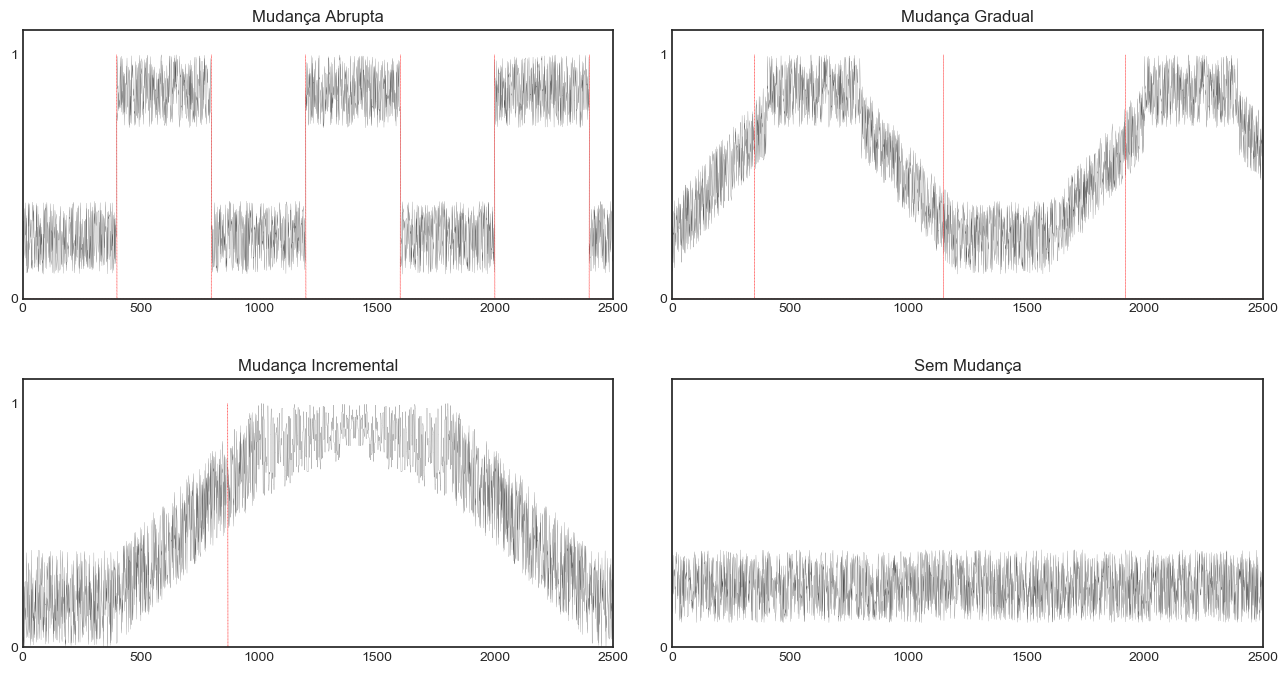
\includegraphics[width=\textwidth]{imagens/conjuntos_dados_sinteticos.png}
    \caption{Representação gráfica dos conjuntos de dados sintéticos.}
    \label{fig:conjuntos_dados_sinteticos}
\end{center}
\end{figure}

\subsection{Critérios de avaliação}

O experimento foi avaliado através da classe \textit{BasicConceptDriftPerformanceEvaluator}, pertencente ao framework MOA.
Esta classe permite mensurar a acurácia e o desempenho de algoritmos de detecção de mudanças de conceito.
Para utilizá-la, é necessário construir uma tarefa do tipo \textit{EvaluateConceptDrift} através da aba \textit{Concept Drift}, presente na tela inicial da aplicação.
Para condução dos experimentos deste trabalho, a tarefa \textit{EvaluateConceptDrift} foi configurada conforme descrito na Tabela \ref{tbl:configuracao_tarefa}.

\newpage

\begin{table}[h]
\centering
\caption{Configuração da classe \textit{BasicConceptDriftPerformanceEvaluator}}
\label{tbl:configuracao_tarefa}
\begin{tabularx}{\textwidth}{ l l X }
\toprule
Parâmetro & Valor & Observação \\
\midrule
learner          & ChangeDetectorLearner  &  Algoritmo a ser testado.               \\
stream           & ARFFFileStream         &  Caminho do arquivo ARFF.  \\
instanceLimit    & $-1$                            &  Desabilita o limite de instâncias.  \\
timeLimit        & $-1$                            &  Desabilita o limite de tempo de execução.  \\
sampleFrequency  & \hspace{2mm}$1$                 &  Imprime a avaliação de cada observação.  \\
\bottomrule
\end{tabularx}
\end{table}

A classe de avaliação utilizada produz diversos indicadores referentes à acurácia e performance do algoritmo executado.
A Tabela \ref{tbl:indicadores_analisado} apresenta os indicadores analisados neste trabalho.


\begin{table}[h]
\centering
\caption{Indicadores analisados}
\label{tbl:indicadores_analisado}
\begin{tabularx}{\textwidth}{ll}
\toprule
Indicador & Observação \\
\midrule
TP       &  \textbf{Tempo de Processamento} por instância (média em seg.). \\
MR       &  \textbf{Mudanças Reais} existentes no conjunto de dados. \\
VP       &  \textbf{Verdadeiro Positivo}. Quantidade de detecções corretas. \\
FP       &  \textbf{Falso Positivo}. Quantidade de detecções errôneas. \\
ATR      &  \textbf{Atraso de detecção}. \\ 
         &  Quantidade média de instâncias entre a mudança de conceito e a detecção. \\
\bottomrule
\end{tabularx}
\end{table}

\subsection{Resultados}

Esta subseção apresenta os resultados obtidos no experimento com dados sintéticos. O experimento realizado utilizou quatro conjuntos de dados, conforme descrito na subseção \ref{sec:configuracao_experimento_sintetico}, e comparou os resultados do método proposto, RBFChain, aos dos algoritmos: ADWIN, CUSUM, DDM, EDDM, EWMA, HDDMA, PageHinkley e SeqDrift1.
Estes algoritmos foram escolhidos por serem tradicionalmente utilizados nas análises comparativas presentes na literatura \cite{Gama:2014:SCD:2597757.2523813, Ross:2012:EWM:2076039.2076307, Barros:RDDM:2017, BlancoCRBDM15:HDDMA:HDDMW:2015} e por apresentarem implementação disponível no MOA.
Os parâmetros padrão dos algoritmos foram aplicados e estão listados na Tabela \ref{tbl:parametros_algoritmos}.

\begin{table}[H]
\centering
\caption{Parâmetros utilizados}
\label{tbl:parametros_algoritmos}
\begin{tabularx}{\textwidth}{lX}
\toprule
Algoritmo & Parâmetros \\
\midrule
RBFChain                  &  $\sigma = 2$; $\lambda = 0.5$; $\alpha = 0.005$; $\delta = 1.0$ \\
ADWIN                     &  $\delta = 0.002$ \\
CUSUM                     &  MinNumInstances = 30; $\delta = 0.005$; $\lambda = 50$ \\
DDM & MinNumInstances = 30; WarningLevel = 2; OutControlLevel = 3 \\
EDDM & --- \\
EWMA &  MinNumInstances = 30; $\lambda = 0.2$ \\
HDDMA & DriftConfidence = $0.001$; WarningConfidence = $0.005$; \\
PageHinkley &  MinNumInstances = 30; $\delta = 0.005; \lambda = 50; \alpha = 1$ \\
SeqDrift1 & delta = 0.01; deltaWarning = 0.1; block = 200 \\
\bottomrule
\end{tabularx}
\end{table}

O primeiro teste utilizou o conjunto de dados sintético sem mudanças de conceito, visando avaliar a tendência de produção de falso positivos.
O resultado desta análise pode ser visto na Tabela \ref{tbl:exp1}.


\begin{table}[h]
\centering
\caption{Resultados dos algoritmos para o conjunto de dados sem mudanças de conceito.}
\label{tbl:exp1}
\begin{tabular}{llllll}

\toprule
Algoritmo              & TP                     & MR                     & VP                     & FP                     & ATR                    \\ 
\midrule
RBFChain               & 0.013                  & 0                      & 0                      & 0                      & ---                    \\ 
ADWIN                  & 0.025                  & 0                      & 0                      & 0                      & ---                    \\ 
CUSUM                  & 0.016                  & 0                      & 0                      & 0                      & ---                    \\ 
DDM                    & 0.014                  & 0                      & 0                      & 0                      & ---                    \\ 
EDDM                   & 0.013                  & 0                      & 0                      & 0                      & ---                    \\ 
EWMA                   & 0.014                  & 0                      & 0                      & 0                      & ---                    \\ 
HDDMA                  & 0.017                  & 0                      & 0                      & 0                      & ---                    \\ 
PageHinkley            & 0.015                  & 0                      & 0                      & 0                      & ---                    \\ 
SeqDrift1              & 0.017                  & 0                      & 0                      & 0                      & ---                    \\ 
\bottomrule


\end{tabular}
\end{table}


Como pode ser observado, todos algoritmos testados demonstraram tolerância a ruídos e não indicaram nenhum falso positivo.
Quanto a performance, o algoritmo proposto obteve a melhor média em tempo de processamento, juntamente com o EDDM.
O comportamento dos algoritmos e do conjunto de dados utilizado é apresentado graficamente na Figura \ref{fig:exp_sem_mudancas}.

\begin{landscape}
\begin{figure}[t]
\begin{center}
    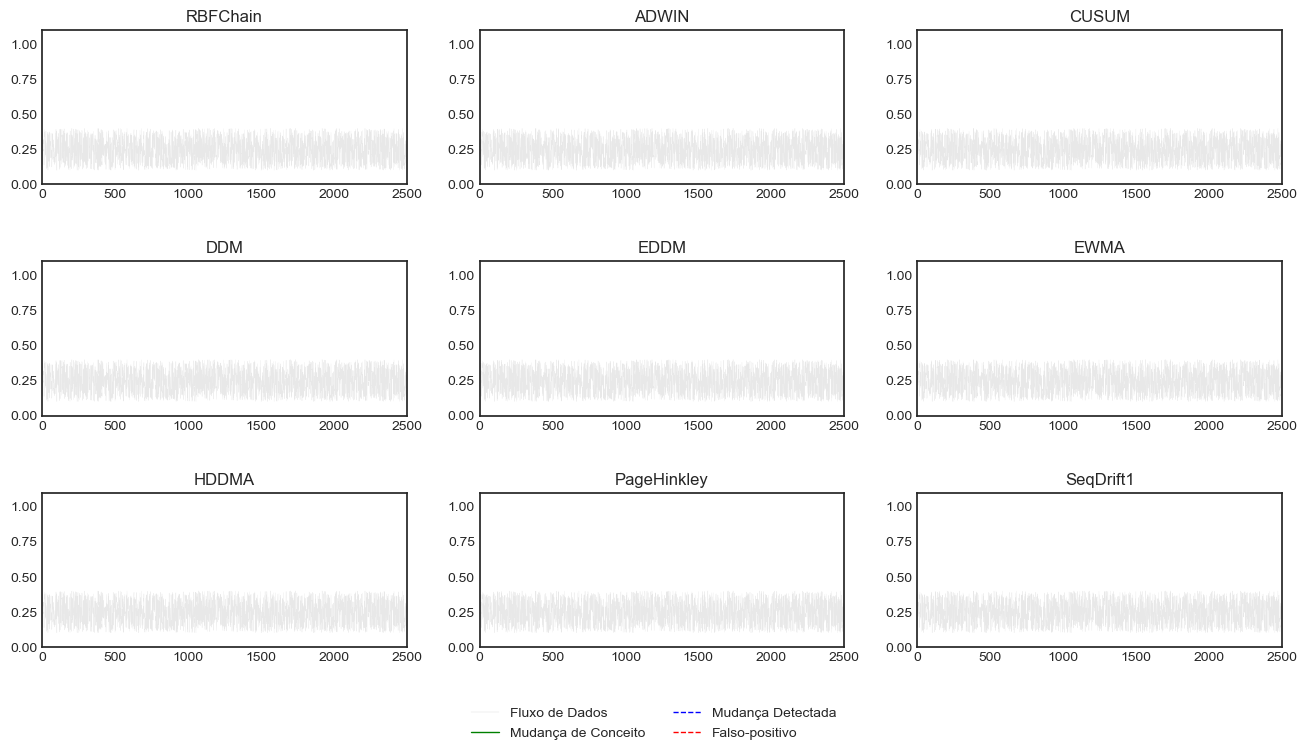
\includegraphics[scale=0.65]{imagens/nochange.png}
    \caption{Comportamento dos algoritmos para o conjunto de dados sem mudanças de conceito.}
    \label{fig:exp_sem_mudancas}
\end{center}
\end{figure}
\end{landscape}

Em seguida, utilizou-se o conjunto de dados com mudanças abruptas.
Os resultados obtidos são apresentados na Tabela \ref{tbl:exp2}.


    \begin{table}[ht]
    \centering
    \caption{Resultados dos algoritmos para o conjunto de dados com mudanças de conceito abruptas.}
    \label{tbl:exp2}
    \begin{tabular}{llllll}

\toprule
Algoritmo              & TP                     & MR                     & VP                     & FP                     & ATR                    \\ 
\midrule
RBFChain               & 0.015                  & 6                      & 5                      & 0                      & 166.67                 \\ 
ADWIN                  & 0.016                  & 6                      & 6                      & 2046                   & 9.00                   \\ 
CUSUM                  & 0.021                  & 6                      & 3                      & 0                      & 68.83                  \\ 
DDM                    & 0.015                  & 6                      & 3                      & 0                      & 38.83                  \\ 
EDDM                   & 0.013                  & 6                      & 0                      & 0                      & ---                    \\ 
EWMA                   & 0.014                  & 6                      & 1                      & 0                      & 1.00                   \\ 
HDDMA                  & 0.014                  & 6                      & 3                      & 0                      & 10.00                    \\ 
PageHinkley            & 0.015                  & 6                      & 1                      & 0                      & 16.17                  \\ 
SeqDrift1              & 0.015                  & 6                      & 5                      & 0                      & 167.50                 \\ 
\bottomrule

    \end{tabular}
    \end{table}


Ao analisar este resultado, verifica-se que os algoritmos RBFChain e SeqDrift1 apresentaram as melhores acurácias, identificando 5 das 6 mudanças existentes, sem produzir nenhum falso positivo.
O método proposto apresentou o terceiro melhor tempo de processamento (TP), com uma pequena diferença para o primeiro.
Os outros algoritmos analisados apresentaram acurácia inferior, e o algoritmo ADWIN se mostrou hipersensível.

Os resultados deste teste são demonstrados graficamente na Figura \ref{fig:exp_abrupta}. Nesta imagem, as linhas sólidas na cor verde representam as mudanças de conceito existentes no conjunto de dados analisado. As linhas tracejadas azuis representam mudanças de conceito identificadas corretamente e as linhas tracejadas de cor vermelha representam falso positivos.

\begin{landscape}
\begin{figure}[h]
\begin{center}
    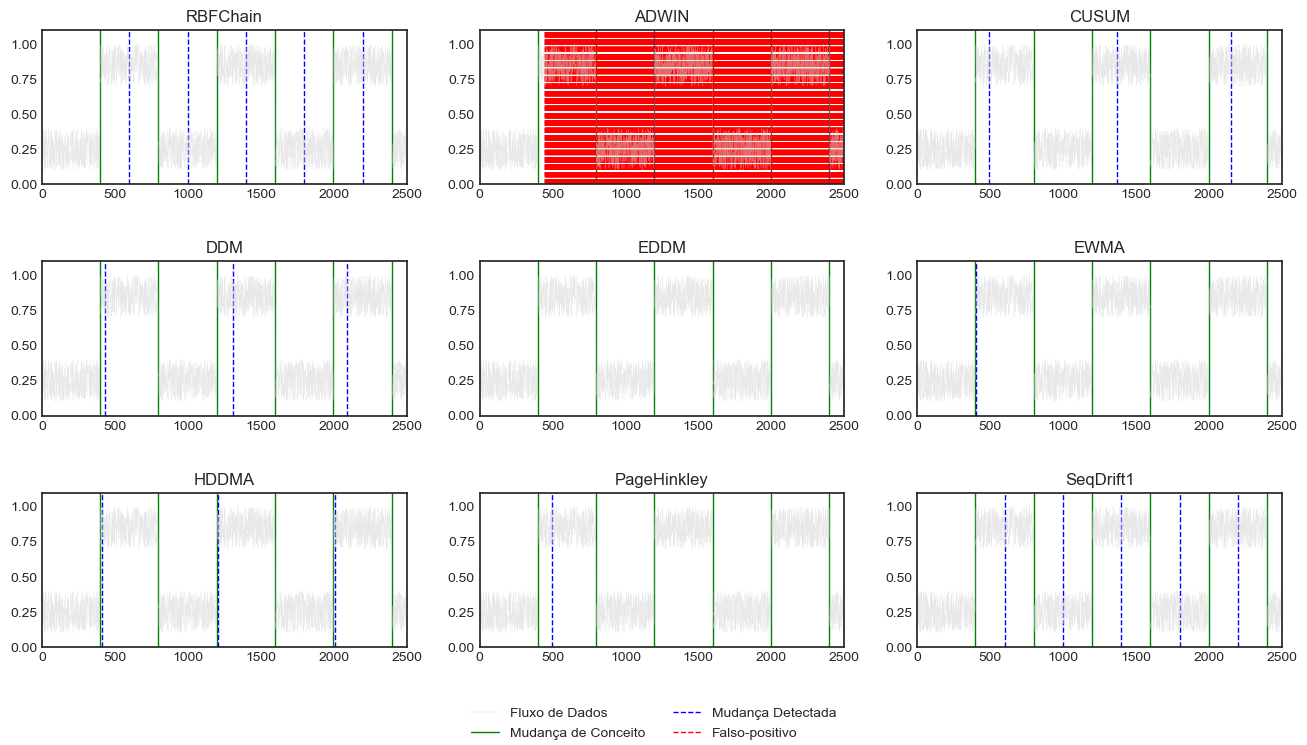
\includegraphics[scale=0.65]{imagens/abrupt.png}
    \caption{Comportamento dos algoritmos para o conjunto de dados com mudanças de conceito abruptas.}
    \label{fig:exp_abrupta}
\end{center}
\end{figure}
\end{landscape}

Posteriormente, empregou-se o conjunto de dados com mudanças de conceito graduais.
O resultado é demonstrado na Tabela \ref{tbl:exp3}.

\begin{table}[ht]
\centering
\caption{Resultados dos algoritmos para o conjunto de dados com mudanças de conceito graduais.}
\label{tbl:exp3}
\begin{tabular}{llllll}

\toprule
Algoritmo              & TP                     & MR                     & VP                     & FP                     & ATR                    \\ 
\midrule
RBFChain               & 0.011                  & 3                      & 3                      & 0                      & 101.00                 \\ 
ADWIN                  & 0.020                  & 3                      & 3                      & 2209                   & 1.00                   \\ 
CUSUM                  & 0.014                  & 3                      & 2                      & 0                      & 83.33                  \\ 
DDM                    & 0.014                  & 3                      & 1                      & 1                      & 58.33                  \\ 
EDDM                   & 0.013                  & 3                      & 0                      & 0                      & ---                    \\ 
EWMA                   & 0.015                  & 3                      & 0                      & 0                      & ---                    \\ 
HDDMA                  & 0.014                  & 3                      & 2                      & 0                      & 100.67                 \\ 
PageHinkley            & 0.014                  & 3                      & 1                      & 0                      & 22.33                  \\ 
SeqDrift1              & 0.015                  & 3                      & 3                      & 1                      & 194.33                 \\ 
\bottomrule


\end{tabular}
\end{table}

A análise do resultado indica que o RBFChain obteve a melhor acurácia, identificando todas as três mudanças de conceito, sem produzir falso positivos.
O algoritmo SeqDrift1 apresentou a segunda melhor acurácia, pois também detectou as três mudanças corretamente, entretanto, apresentou um falso positivo e uma taxa de atraso significativamente maior.
Os algoritmos CUSUM e HDDMA apresentaram uma acurácia média, ao identificar duas mudanças corretamente, sem incidência de falso positivos.
Os outros algoritmos apresentaram uma baixa acurácia e o ADWIN mostrou-se, novamente, hipersensível.
Por fim, o algoritmo proposto também apresentou o melhor resultado em relação ao tempo de processamento.

O conjunto de dados e a execução de cada algoritmo estão representadas graficamente na Figura \ref{fig:exp_gradual}.

\begin{landscape}
\begin{figure}[ht]
\begin{center}
    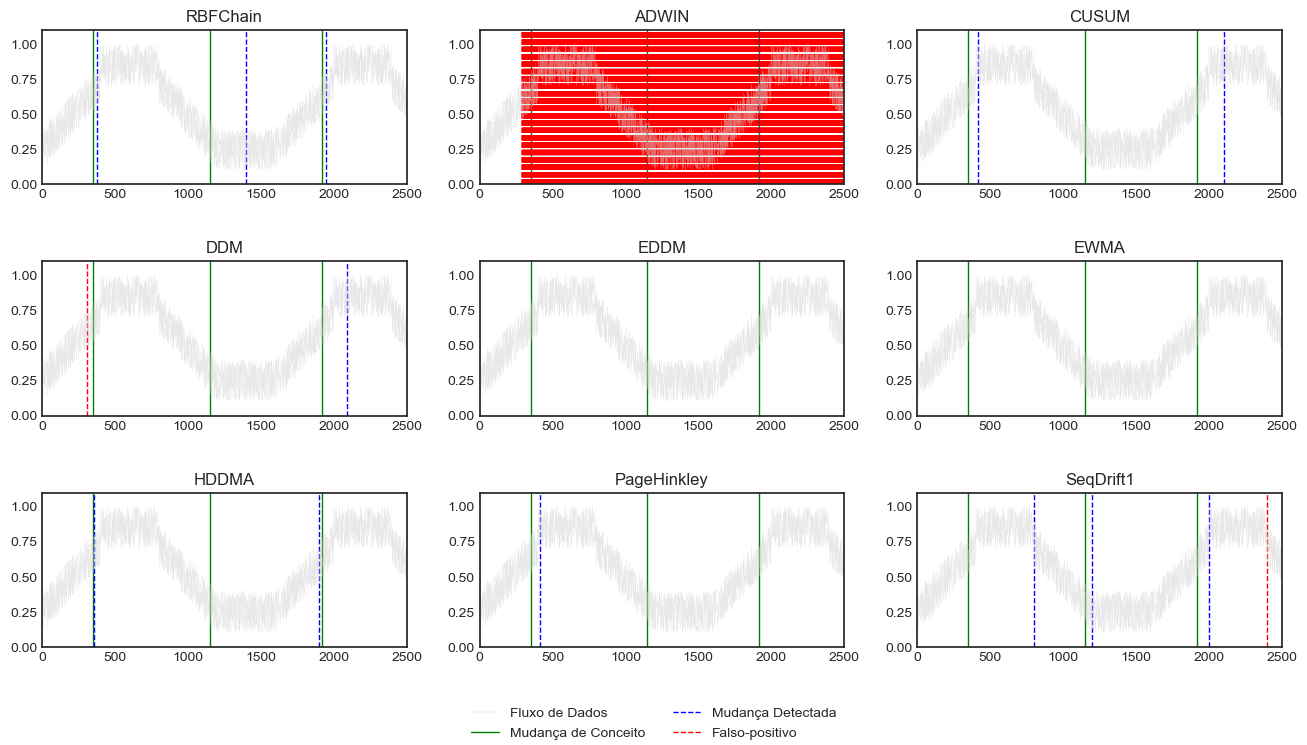
\includegraphics[scale=0.65]{imagens/gradual.png}
    \caption{Comportamento dos algoritmos para o conjunto de dados com mudanças de conceito graduais.}
    \label{fig:exp_gradual}
\end{center}
\end{figure}
\end{landscape}

O último teste utilizou o conjunto de dados com mudanças de conceito incrementais.
O resultado deste teste pode ser visto na Tabela \ref{tbl:exp4}.

\begin{table}[ht]
\centering
\caption{Resultados dos algoritmos para o conjunto de dados com mudanças de conceito incrementais.}
\label{tbl:exp4}
\begin{tabular}{llllll}

\toprule
Algoritmo              & TP                     & MR                     & VP                     & FP                     & ATR                    \\ 
\midrule
RBFChain               & 0.020                  & 1                      & 1                      & 2                      & 501.00                 \\ 
ADWIN                  & 0.017                  & 1                      & 1                      & 1923                   & 1.00                   \\ 
CUSUM                  & 0.014                  & 1                      & 1                      & 1                      & 434.00                 \\ 
DDM                    & 0.014                  & 1                      & 1                      & 1                      & 349.00                 \\ 
EDDM                   & 0.013                  & 1                      & 0                      & 0                      & ---                    \\ 
EWMA                   & 0.016                  & 1                      & 0                      & 1                      & ---                    \\ 
HDDMA                  & 0.014                  & 1                      & 1                      & 1                      & 213.00                    \\ 
PageHinkley            & 0.014                  & 1                      & 1                      & 1                      & 449.00                 \\ 
SeqDrift1              & 0.016                  & 1                      & 1                      & 2                      & 331.00                 \\ 
\bottomrule

\end{tabular}
\end{table}

Verifica-se, através da análise do resultado, que a mudança de conceito incremental representa uma dificuldade, pois todos algoritmos que detectaram a mudança existente também produziram falso positivos.

Os métodos RBFChain e SeqDrift1, que apresentaram os melhores resultados nos testes anteriores, tiveram a pior acurácia, pois emitiram dois falsos positivo cada.
Contraditoriamente, os algoritmos que obtiveram menor acurácia em testes passados, indicaram apenas um falso positivo cada.

Diante disso, considera-se o teste inconclusivo e ressalta-se a necessidade de uma investigação mais detalhada sobre a detecção de mudanças de conceito incrementais. Esta investigação, inclusive, consta como um dos trabalhos futuros propostos para esta dissertação.

Os resultados deste teste são demonstrados graficamente na Figura \ref{fig:exp_incremental}.

\begin{landscape}
\begin{figure}[ht]
\begin{center}
    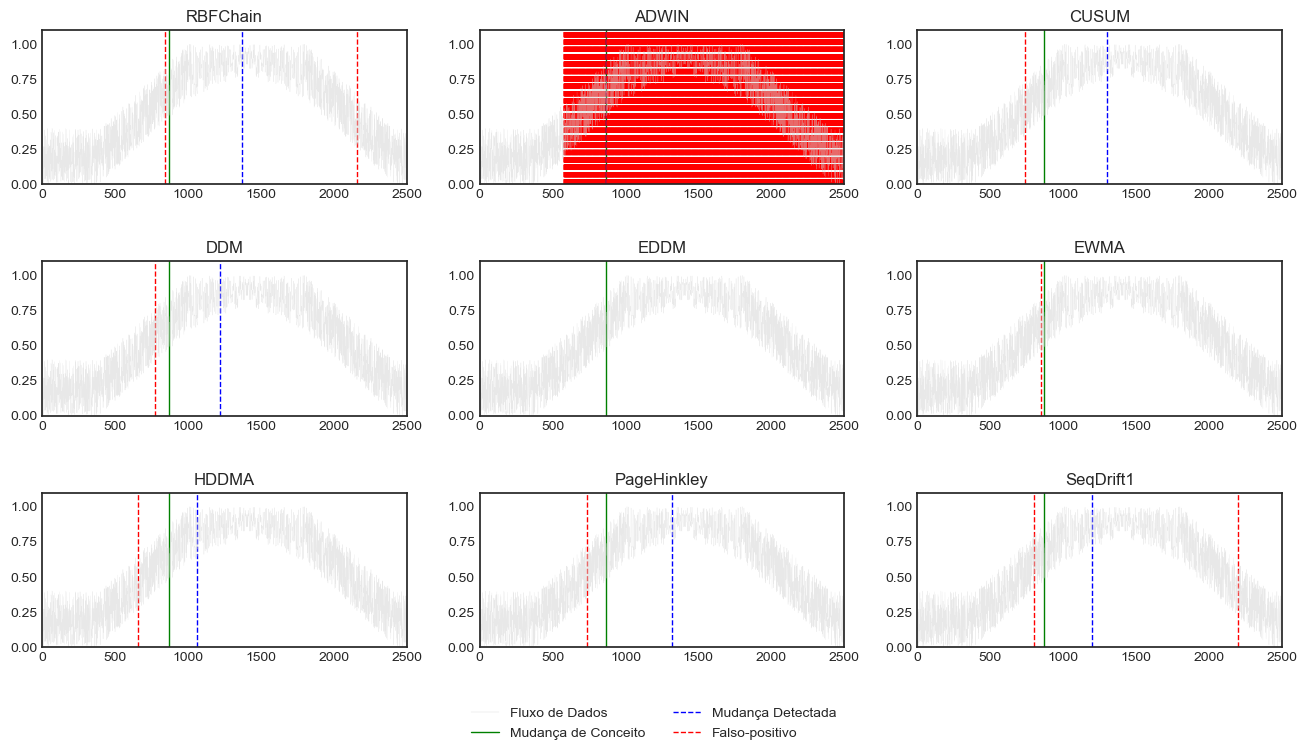
\includegraphics[scale=0.65]{imagens/incremental.png}
    \caption{Comportamento dos algoritmos para o conjunto de dados com mudanças de conceito incrementais.}
    \label{fig:exp_incremental}
\end{center}
\end{figure}
\end{landscape}

Por fim, objetivando verificar a existência de diferenças significativas entre os resultados dos detectores testados, aplicou-se o teste \textit{t-student} com nível de significância $\alpha = 0.05$. Este teste resultou em um \textit{p} valor igual a $0.0007587$, indicando a existência de uma diferença estatisticamente significativa.

Ademais, os resultados obtidos comprovam a viabilidade do método proposto e sugerem que o RBFChain é estatisticamente melhor ou equivalente aos principais detectores presentes na literatura.
Deve-se ressaltar que a técnica desenvolvida se diferencia por detectar mudanças em tempo de execução, de forma computacionalmente eficiente e independente de rótulos, além de modelar as mudanças de conceito em um processo markoviano.

\section{Segundo experimento: classificação de fixações e sacadas}

% \section{Monitoramento Ocular - Fixações e Sacadas}
% \label{sec:monitoramento_ocular}

O monitoramento ocular não é uma técnica experimental recente.
No entanto, o desenvolvimento de tecnologias não invasivas favoreceu o aumento da sua utilização.
Atualmente, a técnica é empregada em diferentes tarefas experimentais \cite{Duchowski_EyeTrackingSurvey}, como, por exemplo:
localização da atenção visual,
detecção de deficiências cognitivas,
avaliação de estratégias de pesquisa visual, entre outras.
Estas tarefas produzem informações que são utilizadas como fator de análise por um vasta gama de pesquisas, em diferentes áreas do conhecimento.

Antes de descrever a atividade de monitoramento ocular, é necessário apresentar alguns conceitos básicos sobre o funcionamento da visão.
Os olhos precisam estar em constante movimento para que a retina possa formar uma imagem nítida.
Este movimento frequente é conhecido como movimento sacádico.
Ao analisar uma imagem ou cena, o olho tende a permanecer fixo durante alguns milissegundos nas áreas mais significativas (fixações);
depois disso, o olho se move em direção a uma nova zona de interesse (sacadas).
Este processo é demonstrado na Figura \ref{fig:exemplo_fixacoes_e_sacadas}, utilizando pontos mais densos para representar as fixações e linhas para as sacadas:

\begin{figure}[H]
    \begin{center}
        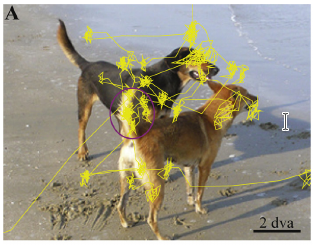
\includegraphics[scale=1]{imagens/exemplo_fixacao_e_sacadas.png}
        \caption{Exemplo de identificação de fixações e sacadas. Fonte: \citeonline{KONIG2014121}.}
        \label{fig:exemplo_fixacoes_e_sacadas}
    \end{center}
\end{figure}

O cérebro não consegue processar as imagens transmitidas pelo sistema visual durante as sacadas, o que causa uma deterioração da imagem formada na retina.
Por esse motivo, o cérebro atribui semântica apenas às imagens formadas durante os períodos de fixação.
Isso implica que o estudo das fixações é essencial para a compreensão e interpretação dos movimentos oculares.

Portanto, é fundamental utilizar técnicas automatizadas para classificar fixações e sacadas durante a análise de trajetórias oculares.
A literatura dispõe de diversos algoritmos para realização desta tarefa.
As técnicas mais utilizadas realizam a classificação com base em limites de velocidade e/ou aceleração,
pois estes valores são significativamente maiores durante as sacadas \cite{Otero_Saccades_and_microsaccades}.
Enquanto outros algoritmos realizam a classificação através de medidas como densidade, dispersão ou áreas de interesse.

Contudo, a aplicação de diferentes algoritmos em uma mesma trajetória ocular pode produzir resultados divergentes, pois os métodos disponíveis na literatura são afetados pela escolha dos parâmetros e pelas características dos dados em análise (frequência, amplitude, etc.) \cite{KONIG2014121}.
Consequentemente, a atividade de classificação de fixações e sacadas permanece altamente subjetiva.

Visando solucionar esse problema, \citeonline{KONIG2014121} propõem um novo método de classificação, denominado ClusterFix.
O método proposto apresenta acurácia equivalente ao estado da arte e se diferencia por ser completamente automatizado e independente de parâmetros.
Essas características permitem que a técnica seja utilizada como um padrão referencial,
possibilitando que classificações de trajetórias oculares sejam comparadas entre laboratórios, experimentos e algoritmos.

Todavia, os algoritmos presentes na literatura, incluindo o ClusterFix, não permitem a classificação da trajetória ocular em tempo de execução, pois atuam em lote, através de rotinas computacionalmente custosas.
Diante disso, investigou-se a aplicação do método proposto por esta dissertação, denominado RBFChain, na classificação de fixações e sacadas em atividades de monitoramento ocular.
Esta investigação permitiu confirmar a aplicabilidade do RBFChain em problema reais, além de contribuir para solução de um relevante problema relacionado à área de Neurociência.

Para validar o método proposto, foram utilizados dois conjuntos de dados oriundos do monitoramento de macacos-pregos e os resultados foram comparados com o algoritmo ClusterFix.
As subseções seguintes apresentam a configuração, os critérios de avaliação e os resultados obtidos durante a prática.

\subsection{Configuração do experimento}
\label{sec:configuracao_experimento_fixacoes_sacadas}

O experimento utilizou dois conjuntos de dados produzidos e cedidos, em parceria, pelo Instituto do Cérebro da Universidade Federal do Rio Grande do Norte (UFRN). 
Os conjuntos de dados são denominados, respectivamente, \textit{Dede} e \textit{Juju}, pois representam os resultados do monitoramento ocular de dois macacos-pregos com esses nomes.
Cada conjunto de dados contém $6.200$ observações formadas por pontos, $(x, y)$, que indicam a localização em análise pelos olhos em cada instante de tempo.

O algoritmo RBFChain foi ligeiramente alterado para poder atuar como um classificador de fixações e sacadas. Nesta versão, o algoritmo deixou de verificar a diferença entre o \textit{centro conceito} e o \textit{centro ativo}, passando a analisar apenas se a probabilidade da transição corrente é maior do que $\delta$. Se esta condição for verdadeira, classifica-se o ponto como uma fixação, do contrário, como sacada. 
Em outras palavras, o algoritmo classifica transições consolidadas - entre o mesmo conceito ou entre conceitos - como fixações e transições não consolidadas, como sacadas.
A adaptação é apresentada em pseudocódigo em Algoritmo \ref{alg:rbfchain_adaptado}:

\begin{algorithm}[H]
    \SetAlgoLined
    \Entrada{$evento, \sigma, \lambda, \alpha, \delta$}
    \Saida{$sacada$ ou $fixacao$}
    \Inicio{

     $grupos \longleftarrow ()$\; 
     $grupoAtivo \longleftarrow nulo$\; 
     $grupoConceito \longleftarrow nulo$\;
     $retorno \longleftarrow nulo$\;
     
     \BlankLine
     
     $minAtivacao \longleftarrow \lambda$\;
     \ParaTodo{grupo}{
         $ativacao \longleftarrow gaussiana(evento, grupo, \sigma)$\\
         \Se{$ativacao >= minAtivacao$}{
            $grupoAtivo \longleftarrow grupo$\;
            $minAtivacao \longleftarrow ativacao$\;
         }
    }
    \Se{$grupoAtivo == nulo$}{
        $grupos \longleftarrow evento$\;
        $grupoAtivo \longleftarrow evento$\;
    }
    
    \BlankLine
    
    \Se{$grupoConceito == nulo$}{
        $grupoConceito \longleftarrow grupoAtivo$\;
    }
    
    \BlankLine
         
    $probabilidade \longleftarrow markov(grupoConceito, grupoAtivo, \alpha)$\;

    \BlankLine
    

    \Se{$probabilidade < \delta$}{
        $retorno \longleftarrow sacada$\;
    }
    \Senao{
        $grupoConceito \longleftarrow grupoAtivo$\;
        $retorno \longleftarrow fixacao$\;
    }

    \BlankLine

    \Retorna{$retorno$}\;
    }

    \caption{\textsc{RBFChain-Adaptado}}
    \label{alg:rbfchain_adaptado}
\end{algorithm}
\vspace{7pt}

Contudo, a implementação presente do RBFChain atua sobre séries univariadas, logo foi necessário converter os pontos dos conjuntos de dados em valores únicos.
Esta conversão foi feita atráves do cálculo da distância Euclidiana de cada ponto em relação ao ponto $(0, 0)$.
Este novo conjunto de dados, formado pelas distâncias, foi utilizado pelo algoritmo.

As métricas utilizadas para validar os resultados do RBFChain - acurácia, precisão e \textit{recall}, necessitam dos rótulos corretos das classificações para serem calculadas. Estes rótulos foram obtidos a partir da implementação oficial, em MATLAB, do algoritmo ClusterFix \cite{KONIG2014121}, utilizado como padrão referencial por esta dissertação.

Por fim, a Figura \ref{fig:trajetorias} demonstra graficamente as trajetórias dos conjuntos de dados analisados.
Na imagem, a trajetória é representada por uma linha sólida verde, e os pontos de \textit{início} e \textit{fim} por marcadores textuais.

\begin{figure}[ht]%
\centering
\subfigure[Trajetória \textit{Dede}]{%
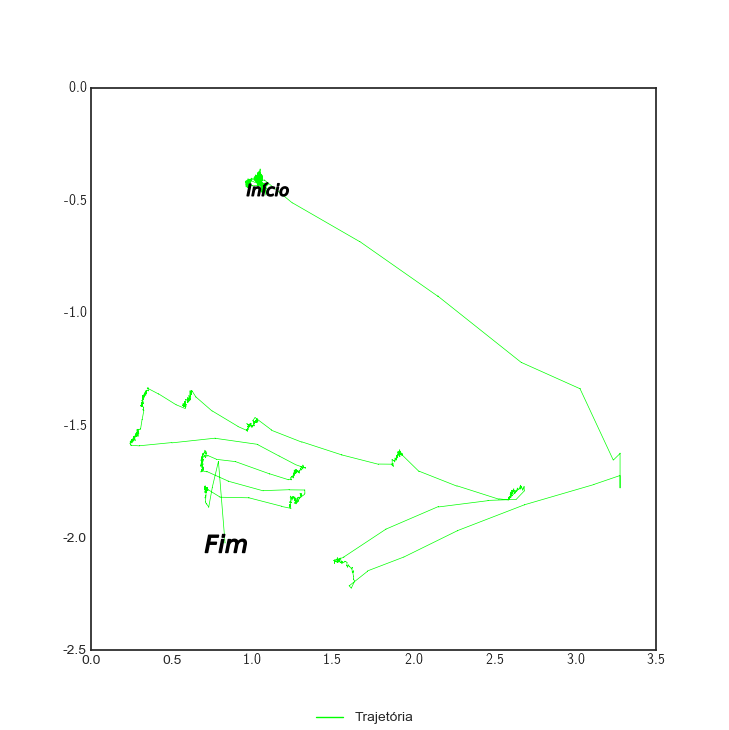
\includegraphics[width=0.45\textwidth]{imagens/trajetoria_dede.png}
}%
\qquad
\subfigure[Trajetória \textit{Juju}]{%
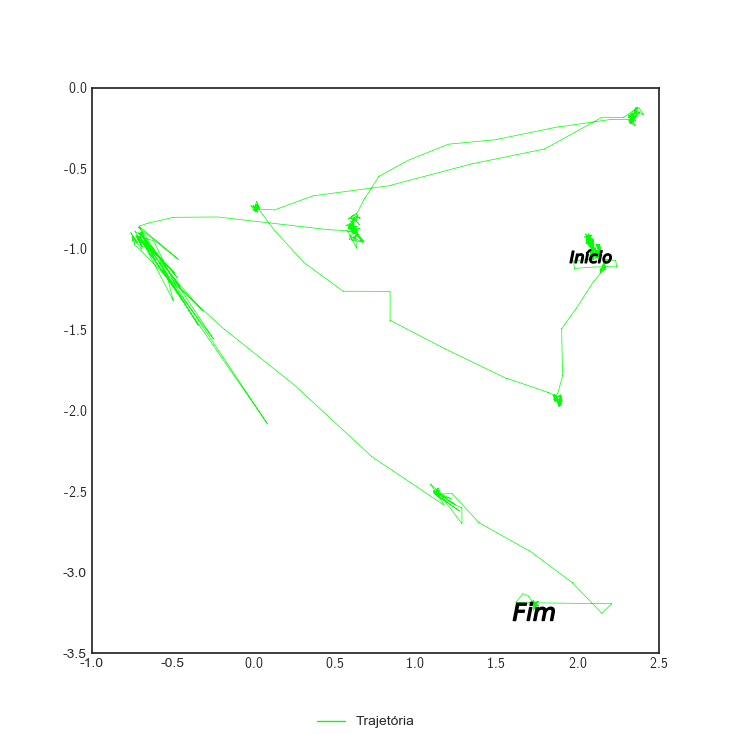
\includegraphics[width=0.45\textwidth]{imagens/trajetoria_juju.png}
}%
\caption{Trajetórias dos conjuntos de dados.}
\label{fig:trajetorias}%
\end{figure}

\subsection{Critérios de avaliação}

Até o presente momento, não existe uma técnica de avaliação consolidada para analisar métodos de classificação de fixações e sacadas.
Por conseguinte, esta dissertação adotou o ClusterFix como padrão referencial, devido as suas características, e os seus resultados foram utilizados como rótulos.
Estes rótulos foram, então, usados para calcular métricas de avaliação para os resultados do RBFChain.
Para tanto, as predições de ambos algoritmos foram transformadas em séries binárias, onde o valor $0$ representa um ponto classificado como sacada, e o valor $1$, uma fixação.

Para entender as fórmulas das métricas utilizadas é preciso conhecer o significado das siglas utilizadas, estas são: Verdadeiros Positivos (TP), Falsos Positivos (FP), Verdadeiros Negativos (TN) e Falsos Negativos (FN).

O parâmetro TP representa a quantidade de verdadeiros positivos que foram classificados corretamente para a classe positiva, o parâmetro TN representa a quantidade de verdadeiros negativos que foram classificados corretamente para a classe negativa. O parâmetro FP representa a quantidade de instâncias que foram classificadas incorretamente para a classe positiva (foram classificadas como positiva mas eram da classe negativa) e o parâmetro FN representa a quantidade de instâncias que foram classificadas incorretamente para a classe negativa (foram classificadas como negativa mas eram da classe positiva).

As métricas utilizadas são apresentadas na Tabela \ref{tbl:metricas_rbfchain}.
Em todas, o melhor valor esperado é $1$ e o pior valor esperado é $0$.

\begin{table}[h]
\centering
\caption{Métricas utilizadas para avaliar as classificações do RBFChain}
\label{tbl:metricas_rbfchain}
\begin{tabularx}{\textwidth}{lXx}
\toprule
Métrica  & Observação & Fórmula \\
\midrule
QP       &  \textbf{Quantidade de Pontos} analisados. & --- \\
AC       &  \textbf{Acurácia}.  &  $\text{AC} = \frac{\text{TP} + \text{TN}}{\text{TP + FP + FN + TN} }$ \\
         & Fração de fixações e sacadas classificadas corretamente.  &  \\

PR       &  \textbf{Precisão}.  &  $\text{PR} = \frac{\text{TP}}{\text{TP + FP} }$ \\
         & Fração das fixações classificadas pelo algoritmo corretamente. &  \\
         
RE       &  \textbf{\textit{Recall}}.  &  $\text{RE} = \frac{\text{TP}}{\text{TP + FN}}$ \\
         & Fração das fixações existentes (rotuladas) que também foram identificadas pelo algoritmo. &  \\
                  
\bottomrule
\end{tabularx}
\end{table}

\subsection{Resultados}

Esta subseção apresenta os resultados obtidos ao aplicar o método de detecção proposto nesta dissertação, denominado RBFChain, na classificação de fixações e sacadas em atividades de monitoramento ocular. 
Para validar a aplicabilidade do método, foram utilizados dois conjuntos de dados, conforme descrito na subseção \ref{sec:configuracao_experimento_fixacoes_sacadas}. 
Os resultados obtidos foram comparados, através de métricas para avaliação de classificadores, aos resultados produzidos pelo algoritmo ClusterFix, que foram utilizados como rótulos.
Por fim, os seguintes parâmetros, definidos de forma empírica, foram empregados: $\sigma = 0.005$, $\lambda = 0.5$, $\alpha = 0.05$ e $\delta = 1.0$.

O primeiro teste utilizou o conjunto de dados \textit{Dede}.
Os resultados obtidos são demonstrados na Tabela \ref{tbl:dede}.

\newpage

\begin{table}[ht!]
\centering
\caption{Resultado da classificação de fixações e sacadas utilizando o RBFChain para o conjunto de dados \textit{Dede}.}
\label{tbl:dede}
\begin{tabular}{llll}

\toprule
QT              & AC                     & PR                     & RE         \\ 
\midrule
$6.200$         & $0.87$                 & $0.98$                 & $0.88$      \\ 
\bottomrule

\end{tabular}
\end{table}

A análise do resultado indica que $87\%$ das fixações e sacadas classificadas pelo RBFChain tiveram a mesma classificação pelo ClusterFix. Ao analisar apenas as fixações identificadas pelo RBFChain, pode-se afirmar que $98\%$ também foram classificadas como fixações pelo ClusterFix. Por fim, dentre todas fixações identificadas pelo ClusterFix, o RBFChain também identificou $88\%$ destas.

As trajetórias traçadas e as fixações identificadas pelos algoritmos ClusterFix e RBFChain estão representadas graficamente na Figura \ref{fig:comparacao_dede}. Nas imagens, a linha verde sólida representa as sacadas e os pontos vermelhos indicam as fixações.

\begin{figure}[ht]%
\centering
\subfigure[ClusterFix - \textit{Dede}]{%
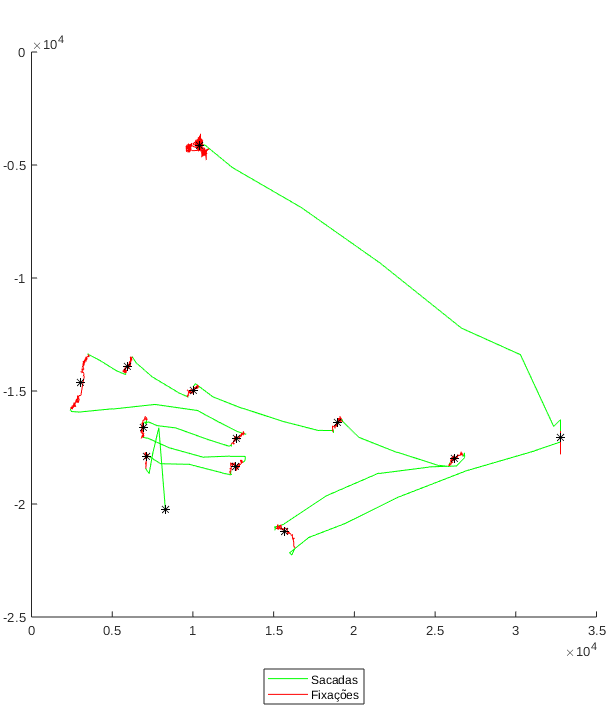
\includegraphics[width=0.45\textwidth]{imagens/dede_clusterfix.png}
}%
\qquad
\subfigure[RBFChain - \textit{Dede}]{%
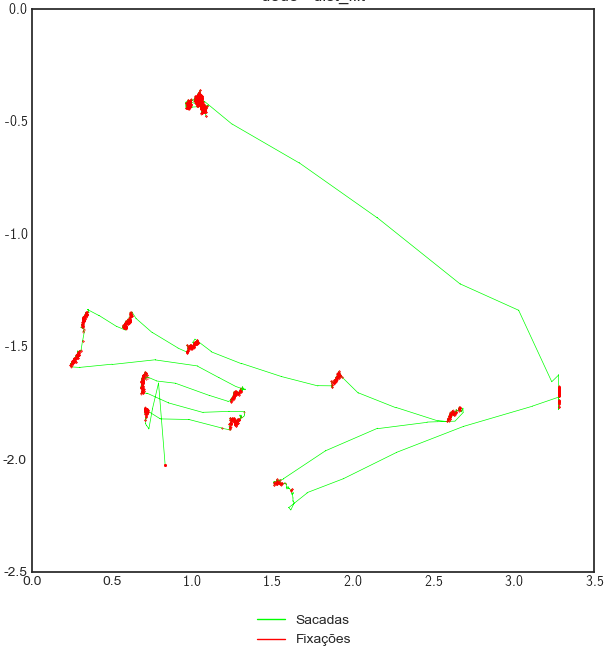
\includegraphics[width=0.45\textwidth]{imagens/dede_rbfchain.png}
}%
\caption{Comportamento dos algoritmos ClusterFix e RBFChain ao analisar o conjunto de dados \textit{Dede}.}
\label{fig:comparacao_dede}%
\end{figure}

O segundo teste utilizou o conjunto de dados \textit{Juju}.
Os resultados obtidos são demonstrados na Tabela \ref{tbl:juju}.

\newpage

\begin{table}[ht!]
\centering
\caption{Resultado da classificação de fixações e sacadas utilizando o RBFChain para o conjunto de dados \textit{Juju}.}
\label{tbl:juju}
\begin{tabular}{llll}

\toprule
QT              & AC                     & PR                     & RE      \\ 
\midrule
$6.200$         & $0.82$                 & $0.98$                 & $0.83$      \\ 
\bottomrule

\end{tabular}
\end{table}

Com base nos resultados, verifica-se que $82\%$ das fixações e sacadas classificadas pelo RBFChain tiveram a mesma classificação pelo ClusterFix. Dentre as fixações identificadas pelo RBFChain, pode-se afirmar que $98\%$ também foram classificadas como fixações pelo ClusterFix. Por fim, dentre as fixações identificadas pelo ClusterFix, o RBFChain também identificou $83\%$ destas.

As trajetórias traçadas e as fixações identificadas pelos algoritmos ClusterFix e RBFChain estão representadas graficamente na Figura \ref{fig:comparacao_juju}.

\begin{figure}[ht]%
\centering
\subfigure[ClusterFix - \textit{Juju}]{%
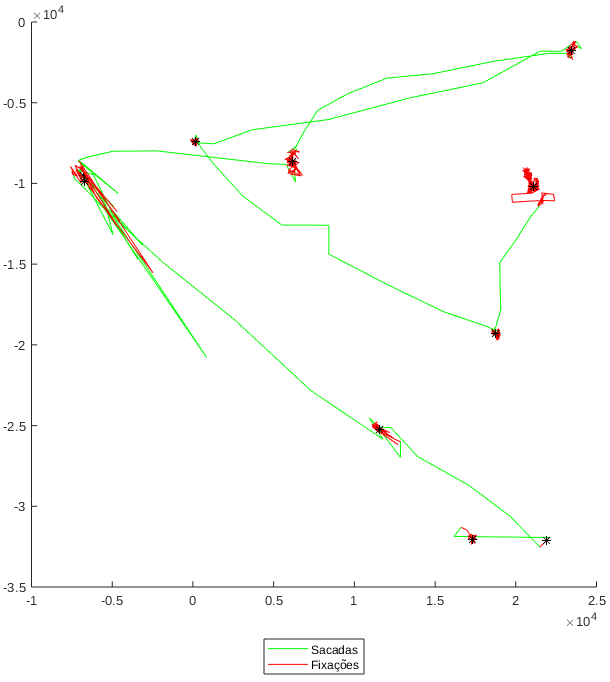
\includegraphics[width=0.45\textwidth]{imagens/juju_clusterfix.png}
}%
\qquad
\subfigure[RBFChain - \textit{Juju}]{%
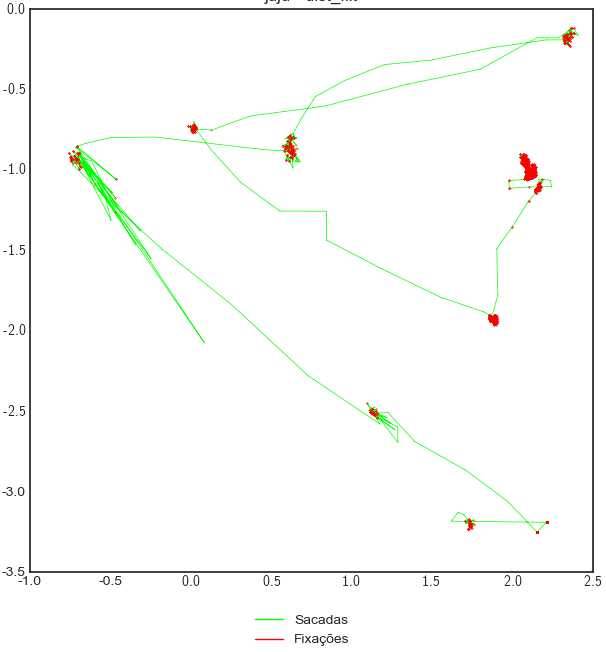
\includegraphics[width=0.45\textwidth]{imagens/juju_rbfchain.png}
}%
\caption{Comportamento dos algoritmos ClusterFix e RBFChain ao analisar o conjunto de dados \textit{Juju}.}
\label{fig:comparacao_juju}%
\end{figure}

Por fim, os resultados obtidos comprovam a aplicabilidade do método proposto ao problema de classificação de fixações e sacadas em atividades de monitoramento ocular.
As métricas obtidas sugerem que o RBFChain é um classificador equivalente ao ClusterFix, considerado estado da arte.
Deve-se ressaltar que o método proposto realiza a classificação dos pontos em tempo de execução, ao passo que o ClusterFix atua em lote, realizando diversas etapas de agrupamento.


\section{Considerações Finais}

Este capítulo abordou em detalhes a avaliação experimental realizada para o método de detecção proposto, denominado RBFChain.
A técnica proposta foi validada através de dois experimentos.
O primeiro experimento utilizou dados sintéticos para realizar uma análise detalhada de sensibilidade, precisão e tolerância ao ruído, confrontando o método proposto com os principais algoritmos disponíveis na literatura.
O segundo experimento aplicou a técnica a um problema real de classificação de fixações e sacadas na atividade de monitoramento ocular, um relevante problema relacionado à área de Neurociência.

\xchapter{Conclusões e Trabalhos Futuros}{} \label{conclusoes_e_trabalhos_futuros}

\section{Discussões}

Este trabalho apresentou um novo método de detecção de mudanças de conceito, denominado RBFChain, baseado em Redes de Função de Base Radial (RBF) e Cadeias de Markov.
O método apresentado se diferencia dos trabalhos existentes por detectar mudanças em tempo de execução, de forma computacionalmente eficiente e independente de rótulos.

O método proposto foi avaliado através de dois experimentos.
O primeiro experimento utilizou dados sintéticos para realizar uma análise detalhada de sensibilidade, precisão e tolerância ao ruído, 
além de comparar os resultados com os principais algoritmos disponíveis na literatura.

O segundo experimento aplicou a técnica desenvolvida a um problema real de classificação de fixações e sacadas na atividade de monitoramento ocular, 
um problema relevante que envolve as áreas de Neurociência e Computação.

Os resultados obtidos sugerem que o RBFChain é estatisticamente melhor ou equivalente aos principais detectores presentes na literatura.
Ademais, o método proposto também apresentou bons resultados quando aplicada ao problema de monitoramento ocular, sendo capaz de classificar fixações e sacadas em tempo real e com precisão equivalente ao estado da arte.

\section{Trabalhos Futuros}

Alguns dos possíveis trabalhos futuros são descritos a seguir:

\begin{itemize}

    \item \textbf{Desenvolvimento de novas estratégias para o cálculo dos parâmetros:} A escolha dos
parâmetros é um fator importante no desempenho do
algoritmo proposto. Novas estratégias para calcular automaticamente estes valores devem ser estudadas.

    \item \textbf{Criação de novas bases de dados experimentais:} Poucas bases de dados reais
e artificiais estão disponíveis para serem usadas em experimentos envolvendo detecção de mudanças de conceito.
Faltam bases que simulem mudanças de conceito em contextos diferentes e com presença de ruídos. 
A criação de um repositório de dados que possa ser usado na validação de algoritmos para detecção de mudanças de conceito pode trazer importantes benefícios para a pesquisa na área.

\item \textbf{Tratamento de contextos incrementais}: Mudanças de conceito com padrão de ocorrência incremental representam uma desafio para os algoritmos de detecção.
No experimento realizado nesta dissertação, por exemplo, todos algoritmos apresentaram algum grau de imprecisão ao analisar este contexto.
Portanto, testes mais elaborados devem ser realizados a fim de avaliar o desempenho do algoritmo RBFChain no tratamento de cenários incrementais.

\end{itemize}

%% Parte pos-textual
\backmatter

% Bibliografia
% É aconselhável utilizar o BibTeX a partir de um arquivo, digamos "biblio.bib".
% Para ajuda na criação do arquivo .bib e utilização do BibTeX, recorra ao
% BibTeXpress em www.cin.ufpe.br/~paguso/bibtexpress
\bibliographystyle{abntex2-alf}
\bibliography{biblio}

% Apendices
% Comente se naoo houver apendices
% \appendix

%\xchapter{Exemplo de Ap\^endice}{} %sem preambulo
%\lipsum
% Eh aconselhavel criar cada apendice em um arquivo separado, digamos
% "apendice1.tex", "apendice.tex", ... "apendiceM.tex" e depois
% inclui--los com:
%\xchapter{Decomposição das séries temporais}{} %sem preambulo
\label{apendice1}
\section{Considerações Iniciais}
Neste apêndice consta as 40 séries temporais utilizadas nos experimentos mostrados no Capitulo \ref{experimentos}. As séries foram divididas em 4 tipos conforme a Tabela \ref{series}, onde o tipo representa um conjunto de 10 séries senoide ou cossenoide, sendo acrescida de ruído ou acrescida de ruído e tendência.
Nas imagens são representadas, a séries original,   seu componente determinístico e seu componente estocástico, os quais foram extraídos após a decomposição.
\section{Séries TIPO 1}
10 séries cossenoide com ruído ao longo da série.
\graphicspath{{imagens/}}
\begin{figure}[H]
\begin{center}
  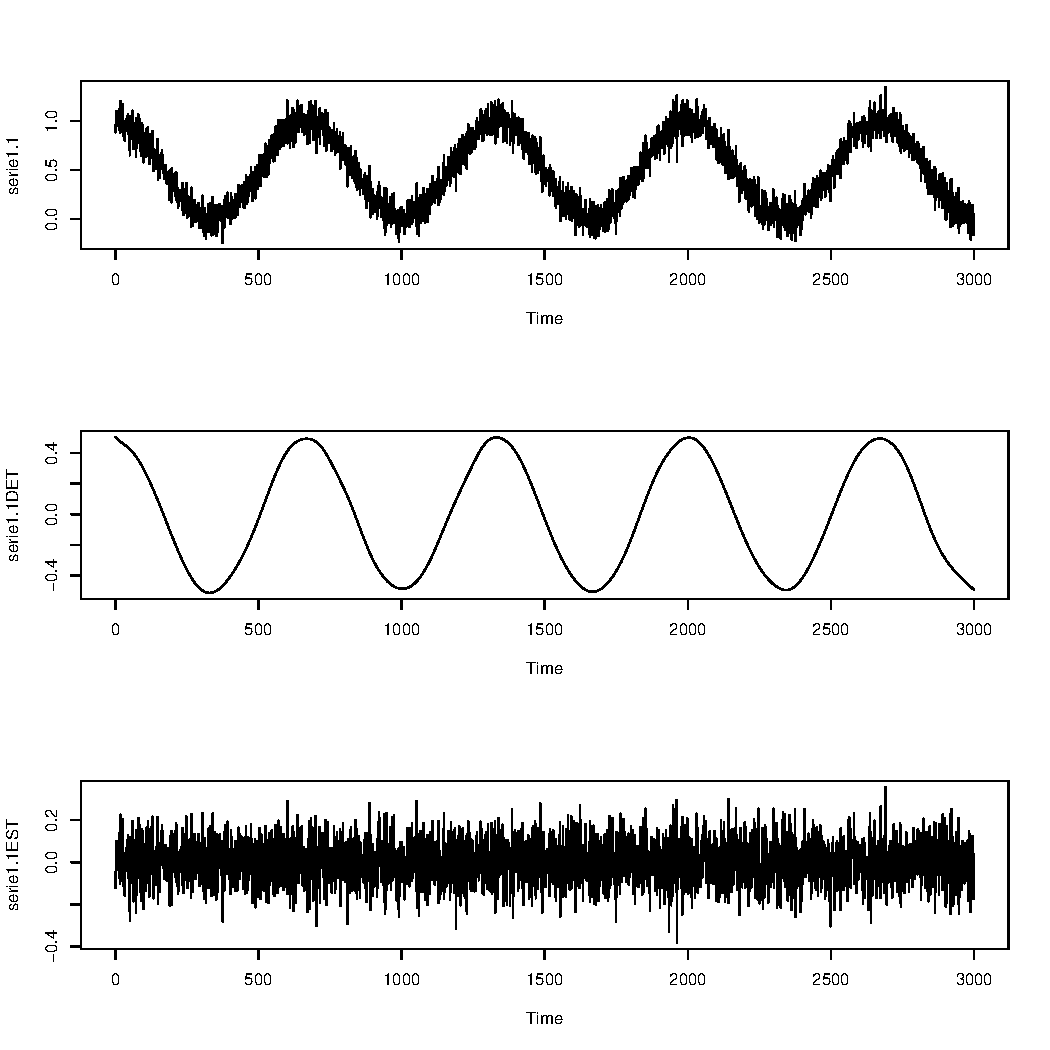
\includegraphics[scale=0.43]{serie1_1.pdf} \quad
  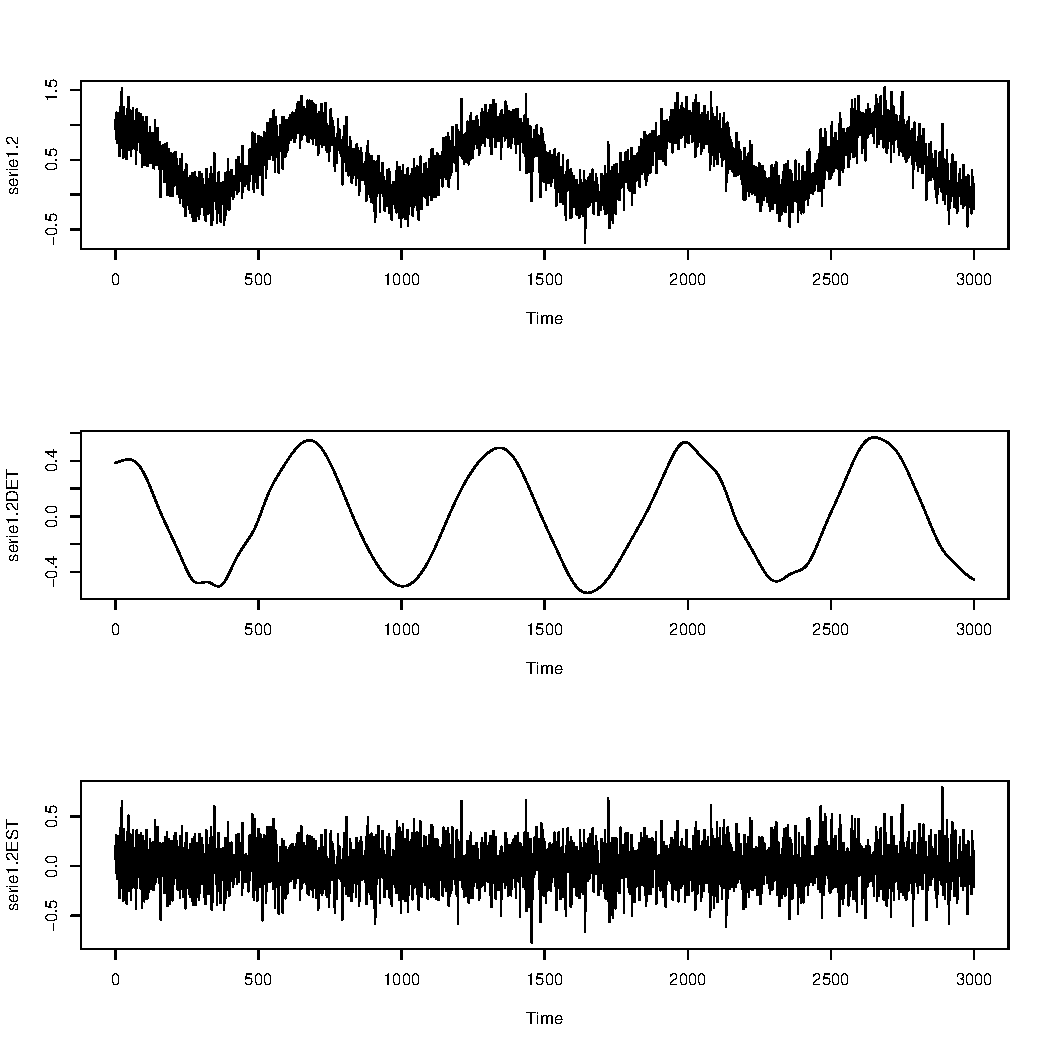
\includegraphics[scale=0.43]{serie1_2.pdf}
  \caption{Série 1.1 e Série 1.2}

\end{center}
\end{figure}

\graphicspath{{imagens/}}
\begin{figure}[H]
\begin{center}
  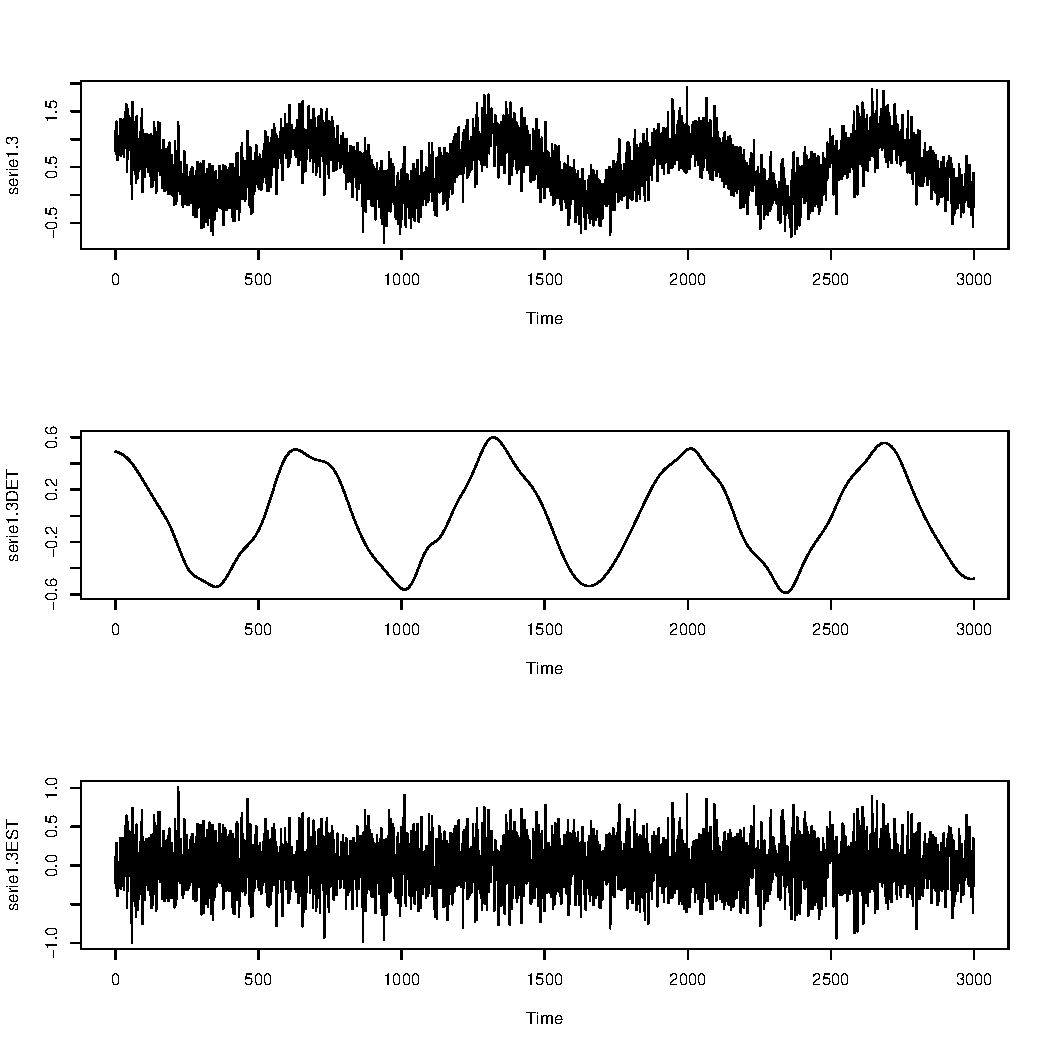
\includegraphics[scale=0.43]{serie1_3.pdf} \quad
  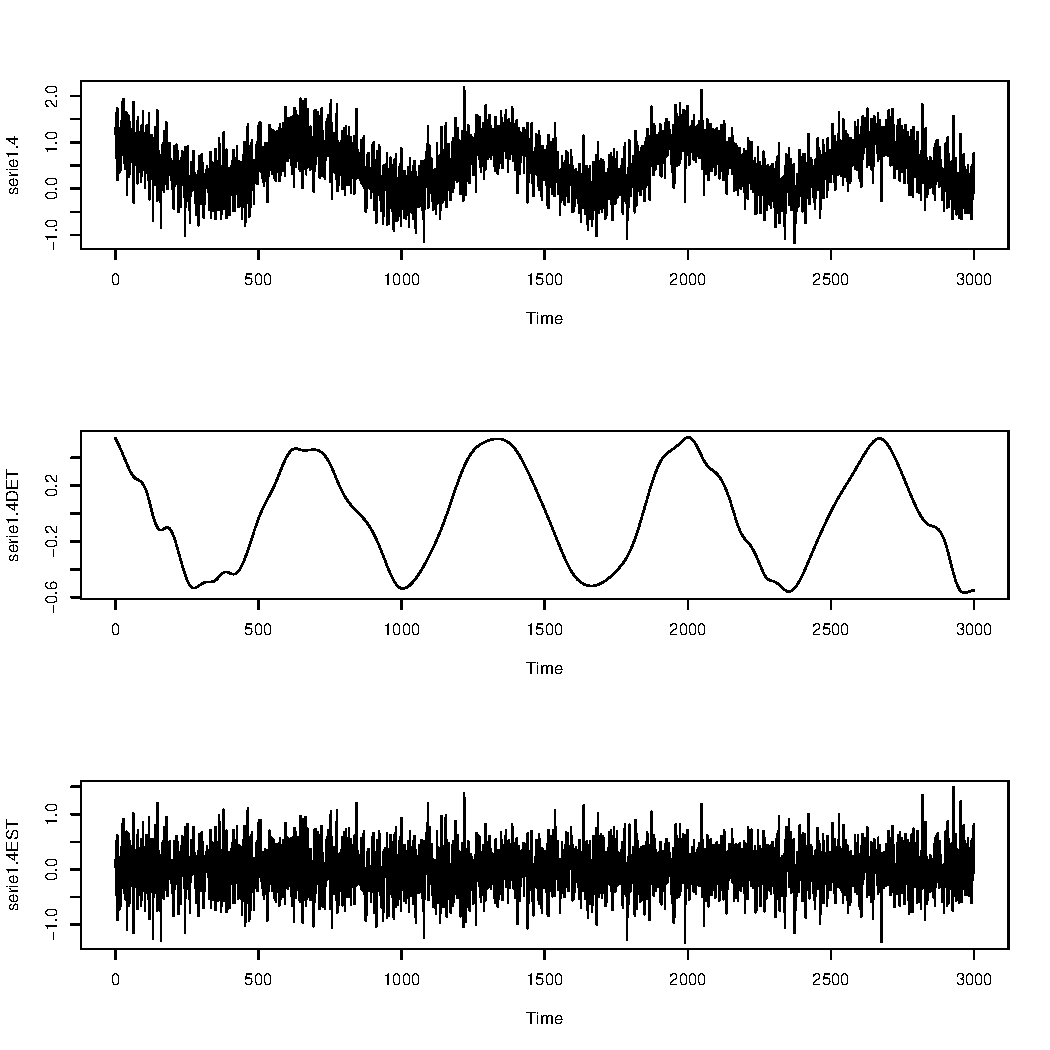
\includegraphics[scale=0.43]{serie1_4.pdf}
  \caption{Série 1.3 e Série 1.4}

\end{center}
\end{figure}

\graphicspath{{imagens/}}
\begin{figure}[H]
\begin{center}
  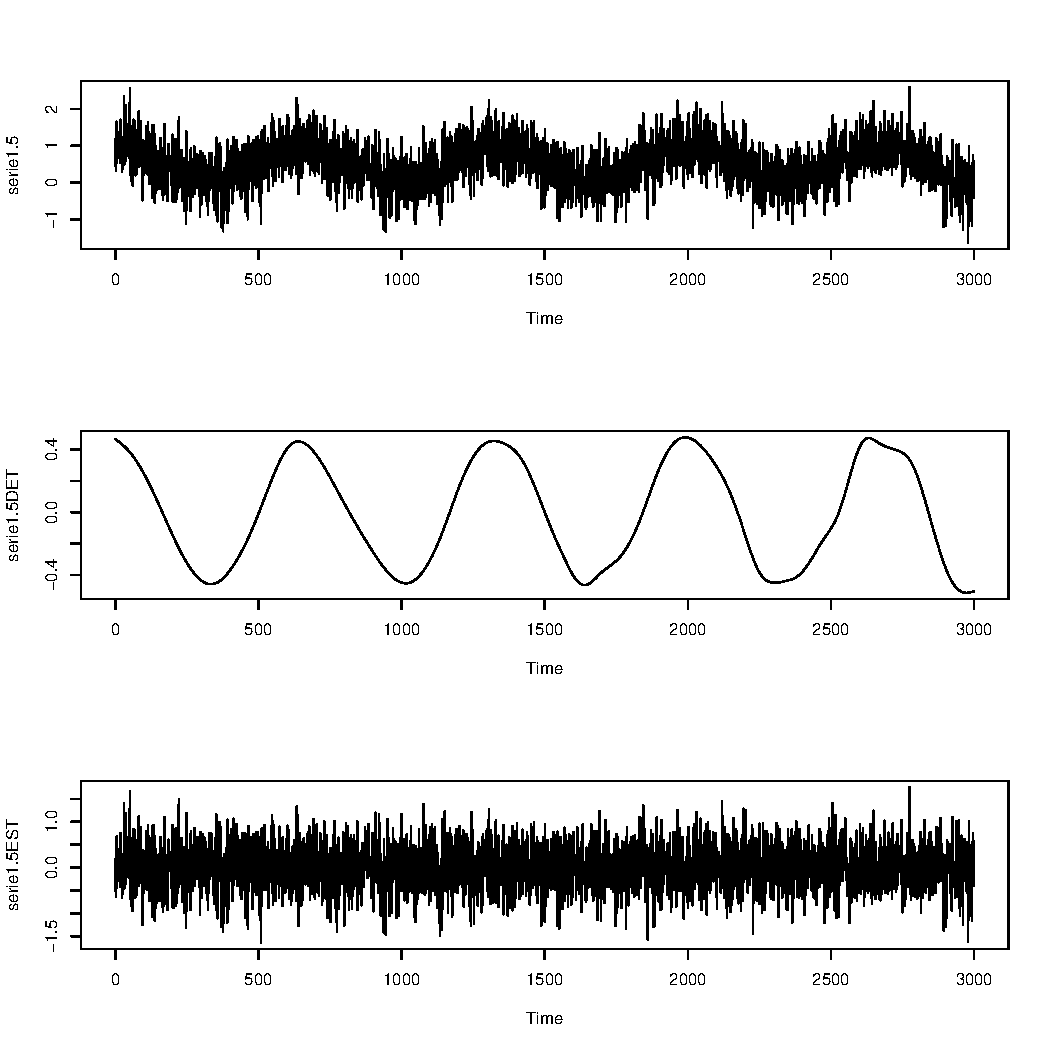
\includegraphics[scale=0.43]{serie1_5.pdf} \quad
  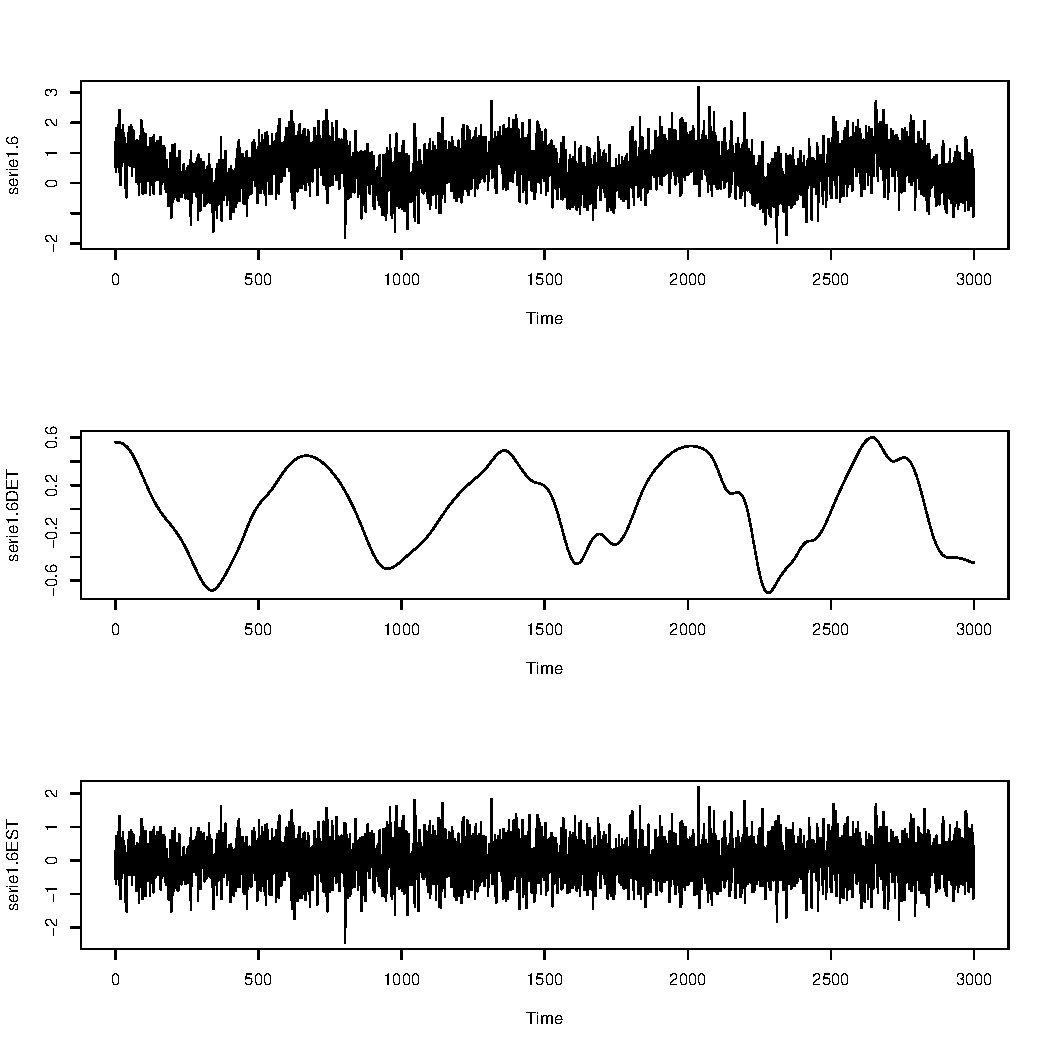
\includegraphics[scale=0.43]{serie1_6.pdf}
  \caption{Série 1.5 e Série 1.6}

\end{center}
\end{figure}

\graphicspath{{imagens/}}
\begin{figure}[H]
\begin{center}
  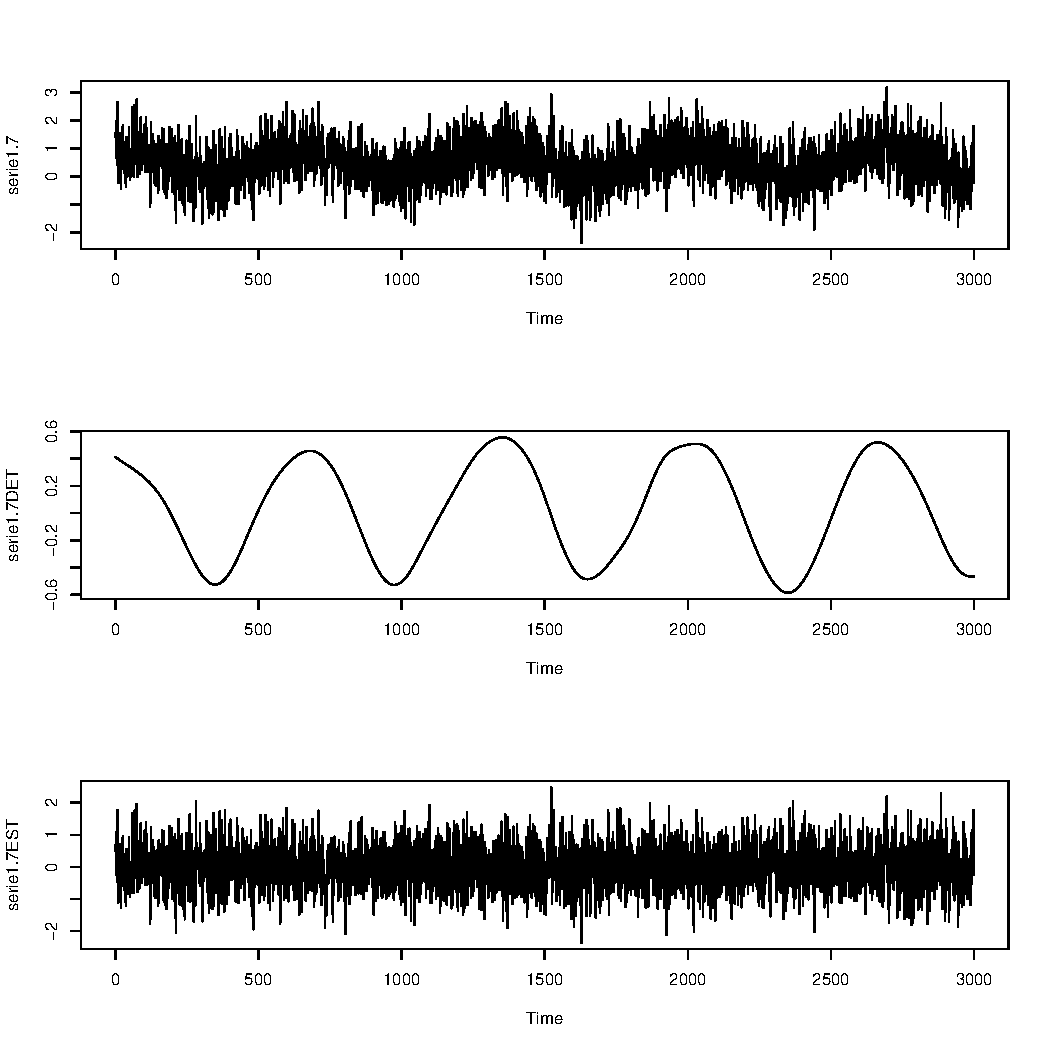
\includegraphics[scale=0.43]{serie1_7.pdf} \quad
  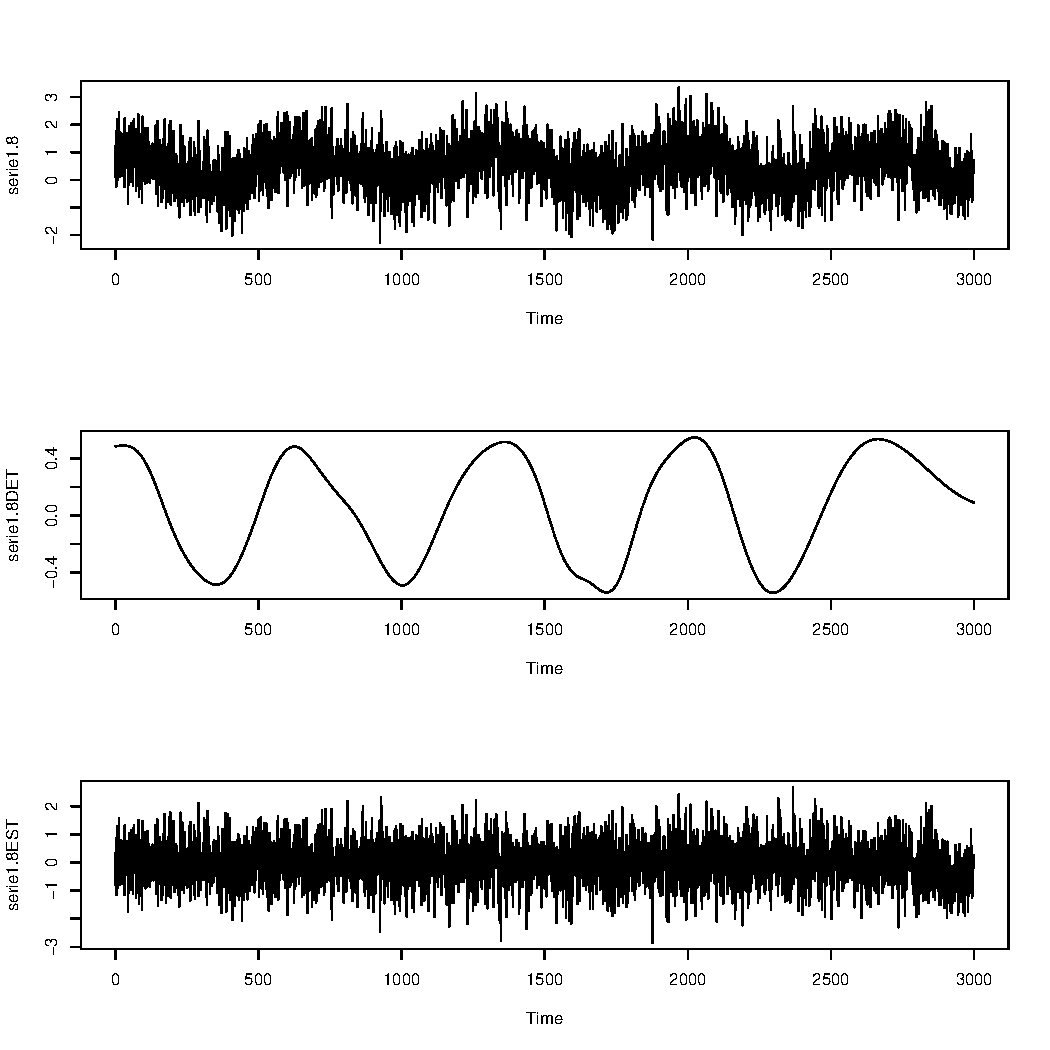
\includegraphics[scale=0.43]{serie1_8.pdf}
  \caption{Série 1.7 e Série 1.8}

\end{center}
\end{figure}

\graphicspath{{imagens/}}
\begin{figure}[H]
\begin{center}
  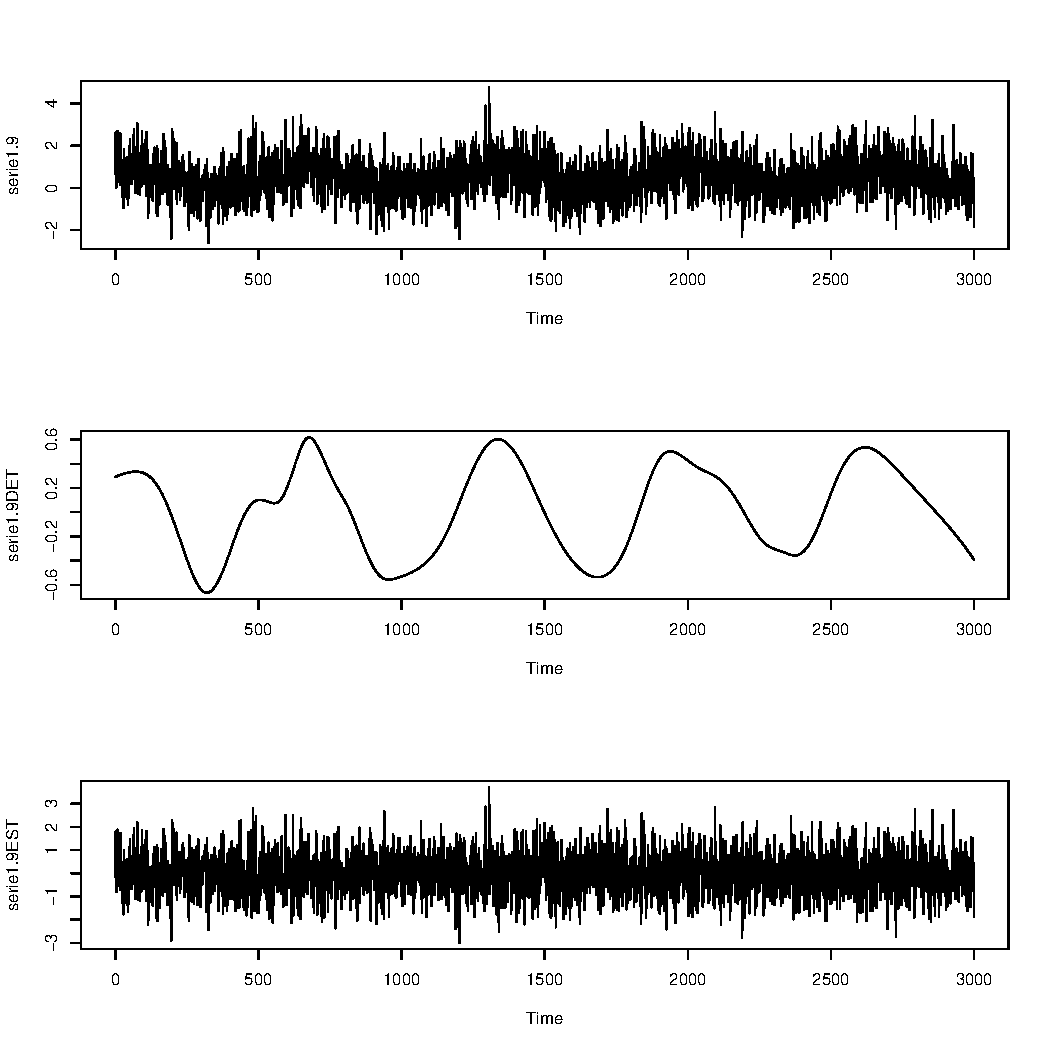
\includegraphics[scale=0.43]{serie1_9.pdf} \quad
  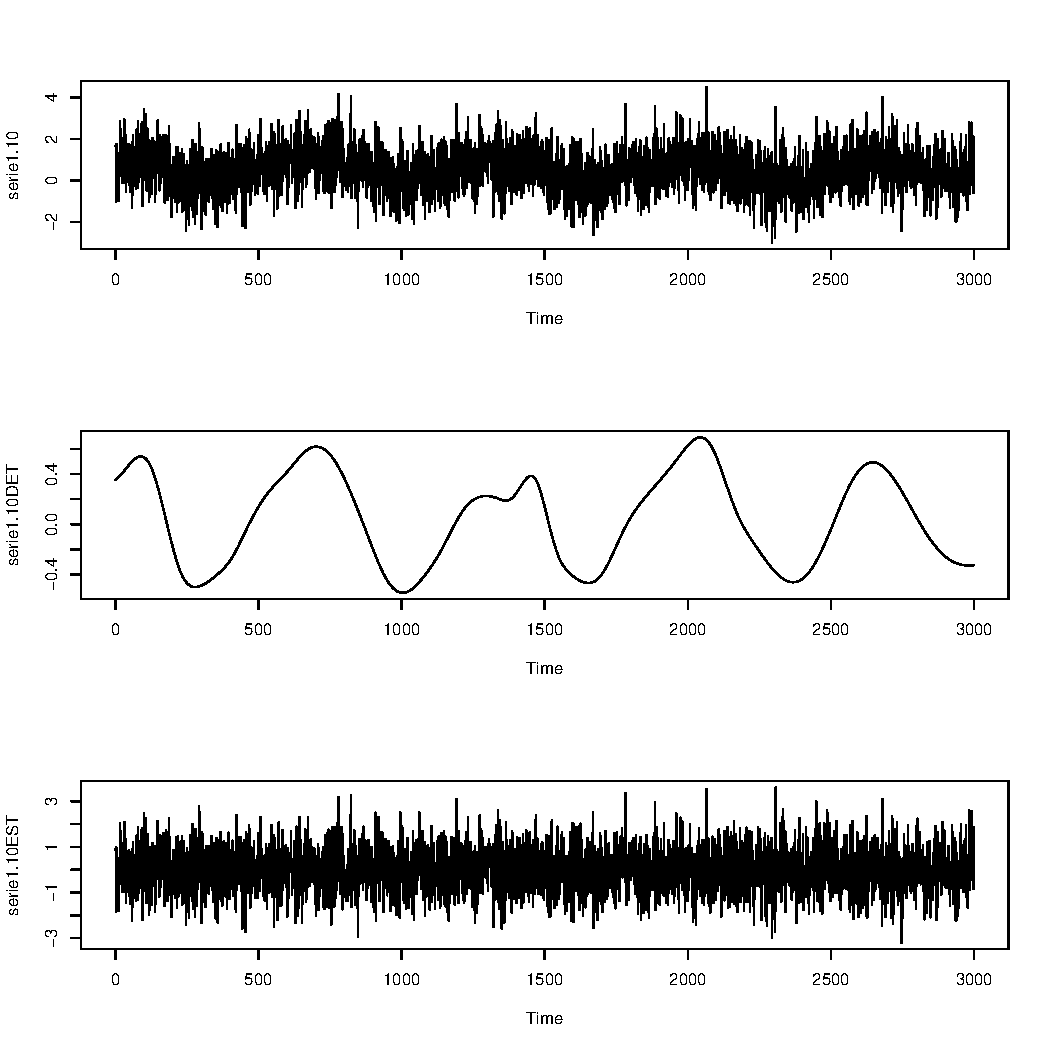
\includegraphics[scale=0.43]{serie1_10.pdf}
  \caption{Série 1.9 e Série 1.10}

\end{center}
\end{figure}

\section{Séries TIPO 2}
10 séries cossenoide com ruído ao longo da série e tendência.
\graphicspath{{imagens/}}
\begin{figure}[H]
\begin{center}
  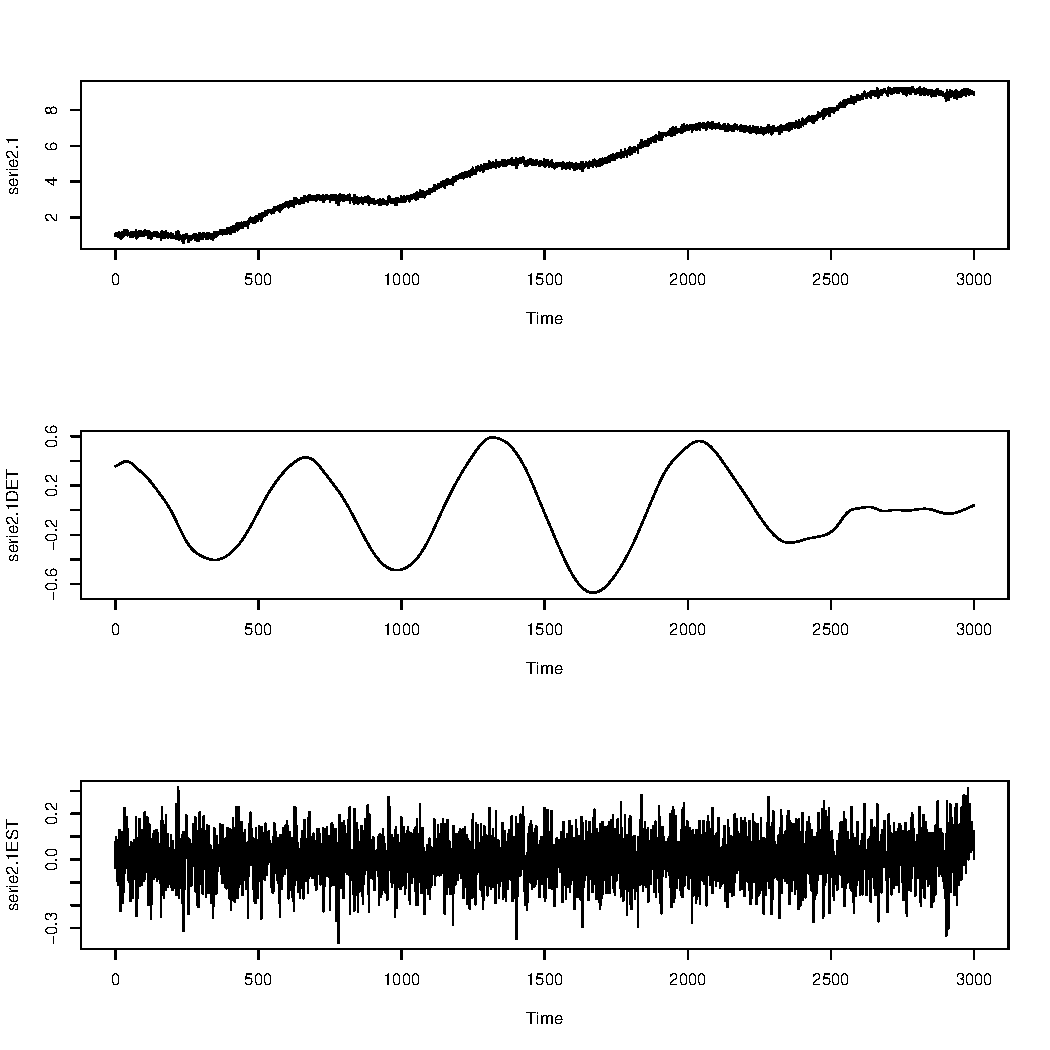
\includegraphics[scale=0.43]{serie2_1.pdf} \quad
  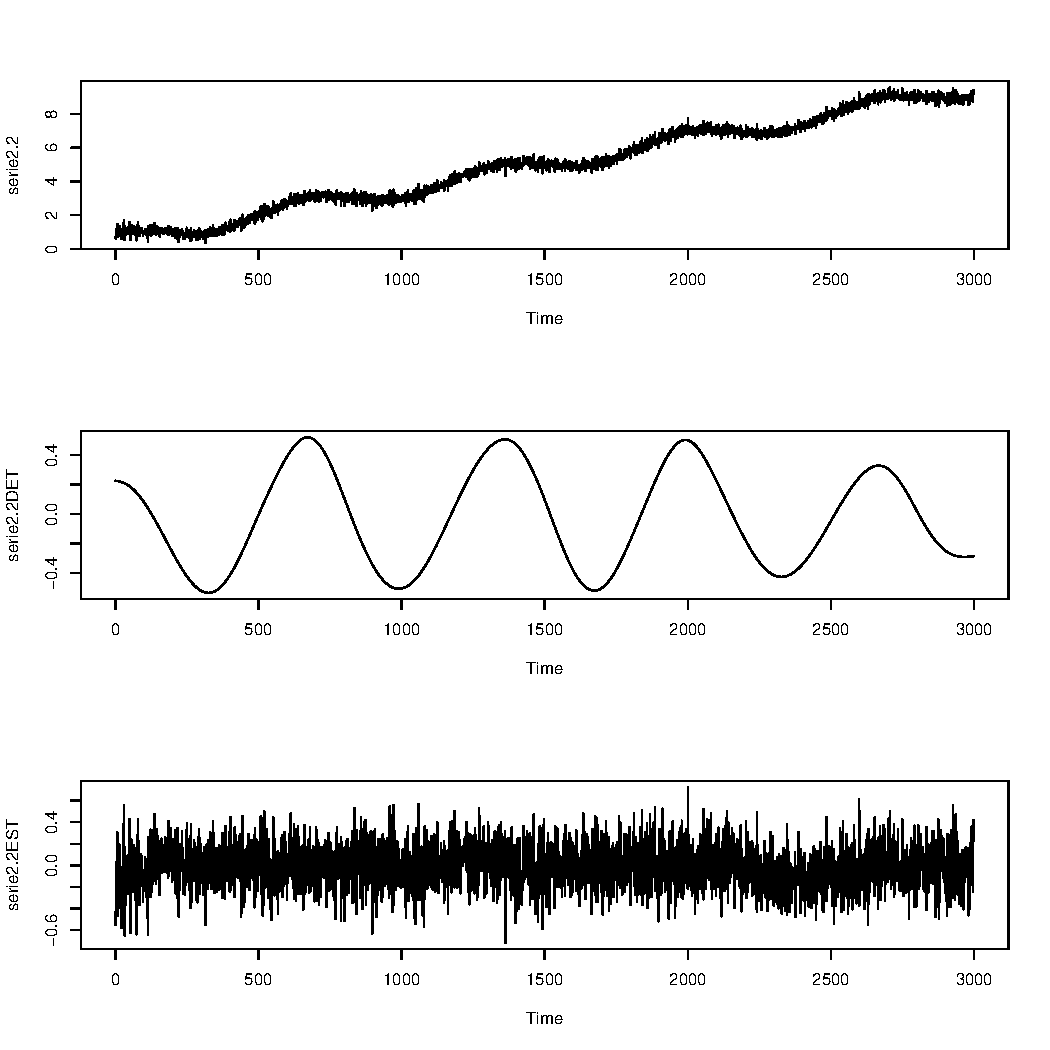
\includegraphics[scale=0.43]{serie2_2.pdf}
  \caption{Série 2.1 e Série 2.2}

\end{center}
\end{figure}

\graphicspath{{imagens/}}
\begin{figure}[H]
\begin{center}
  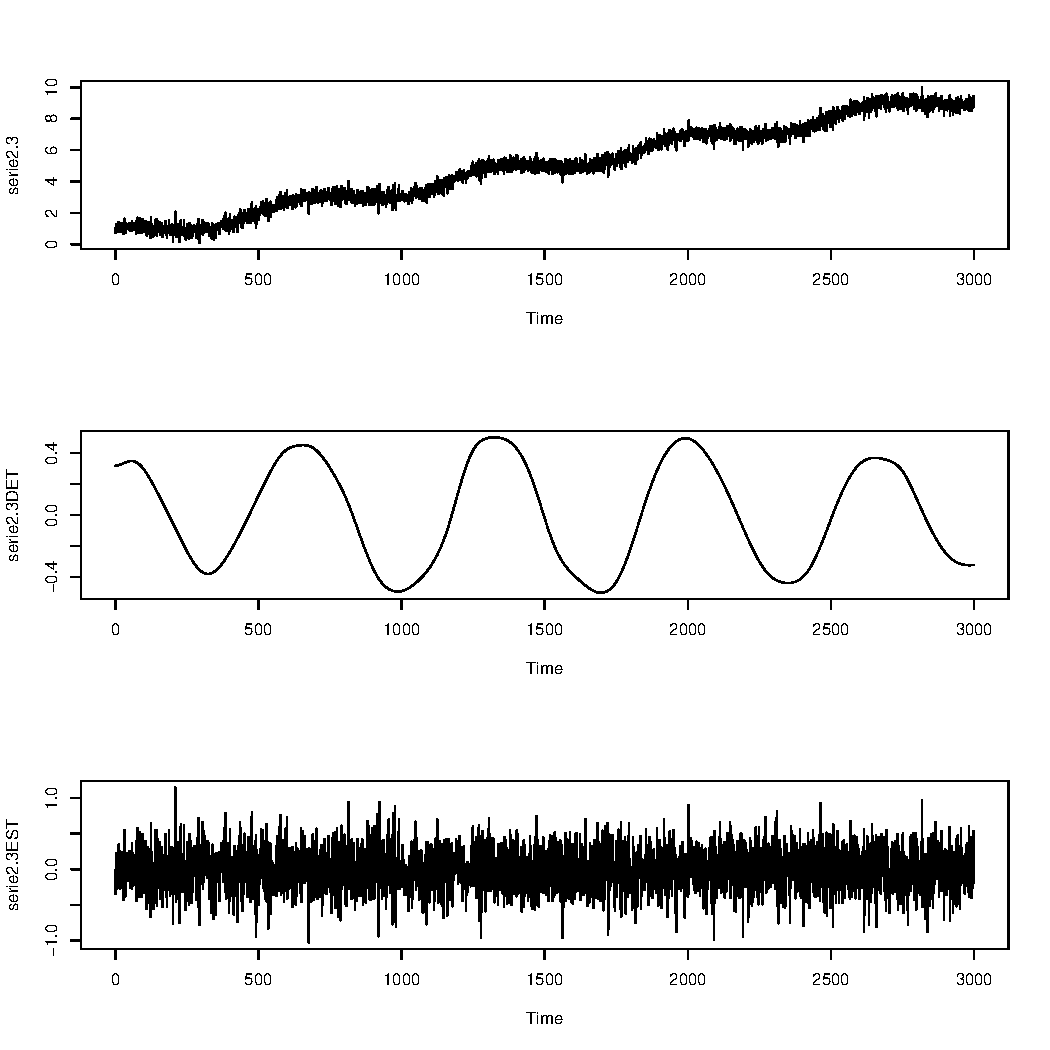
\includegraphics[scale=0.43]{serie2_3.pdf} \quad
  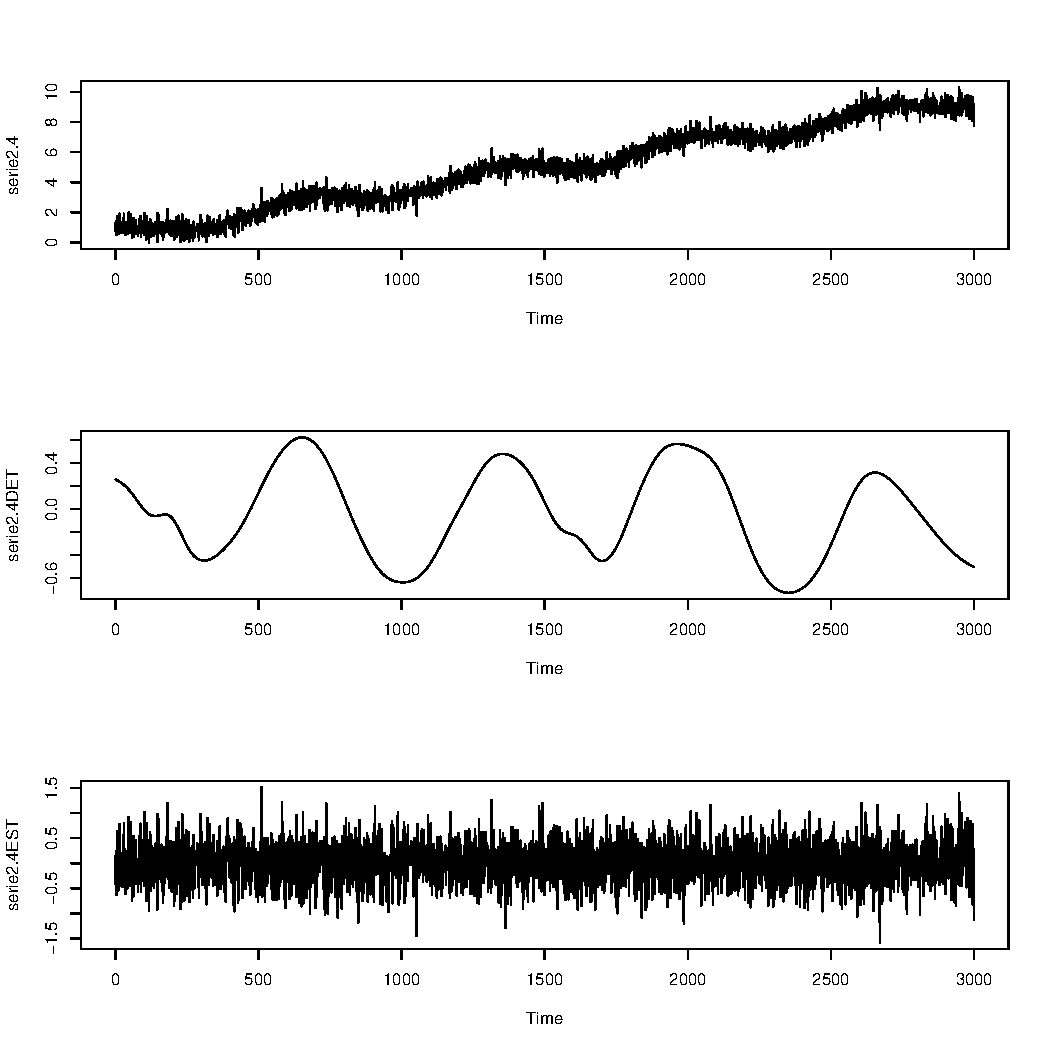
\includegraphics[scale=0.43]{serie2_4.pdf}
  \caption{Série 2.3 e Série 2.4}

\end{center}
\end{figure}

\graphicspath{{imagens/}}
\begin{figure}[H]
\begin{center}
  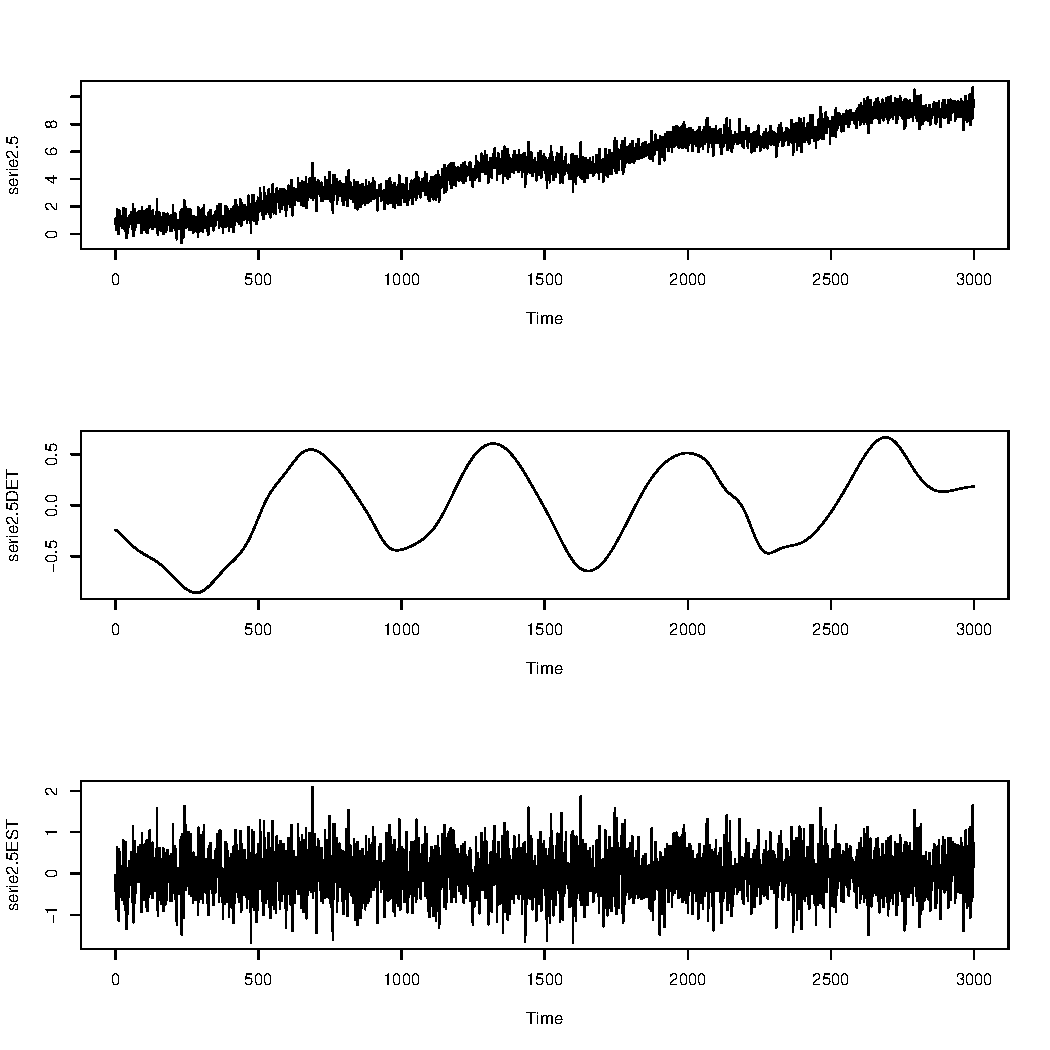
\includegraphics[scale=0.43]{serie2_5.pdf} \quad
  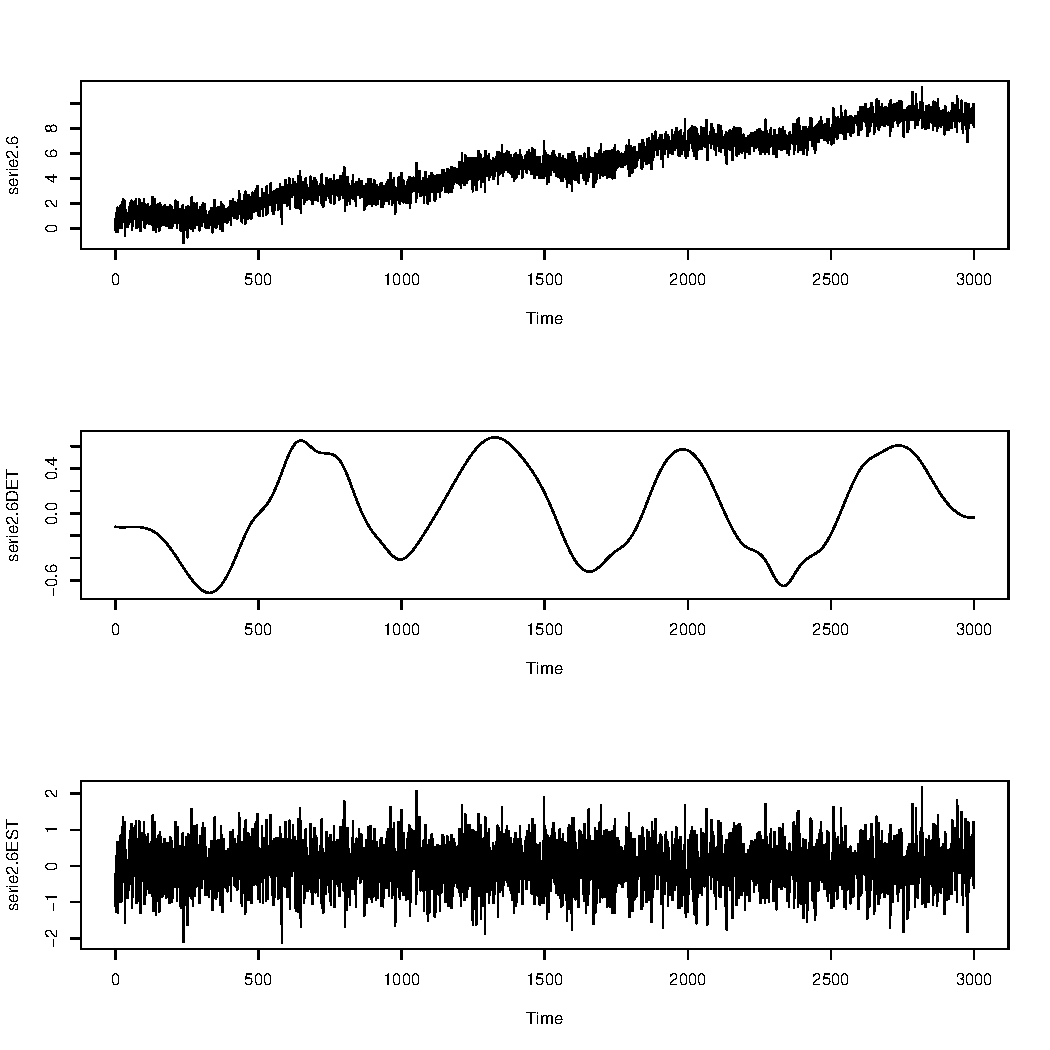
\includegraphics[scale=0.43]{serie2_6.pdf}
  \caption{Série 2.5 e Série 2.6}

\end{center}
\end{figure}

\graphicspath{{imagens/}}
\begin{figure}[H]
\begin{center}
  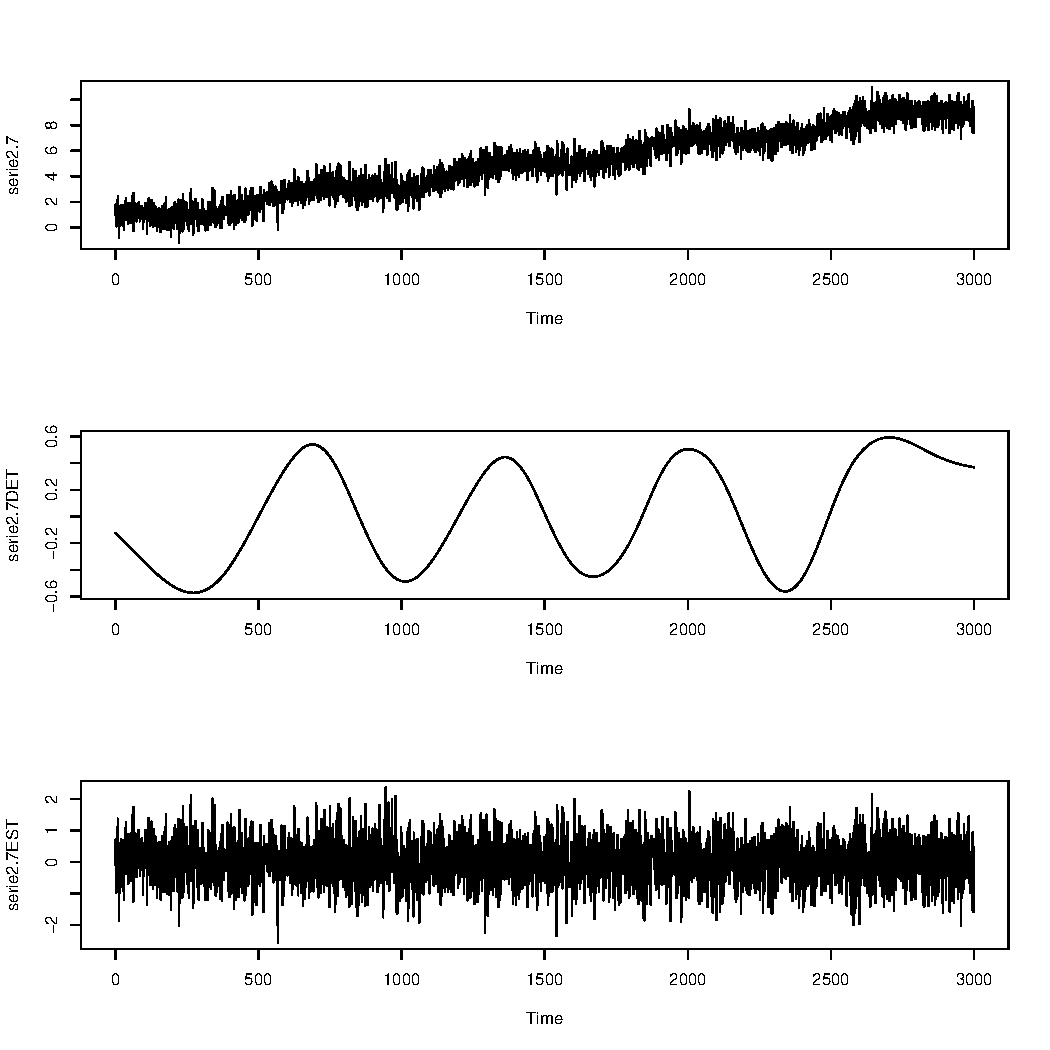
\includegraphics[scale=0.43]{serie2_7.pdf} \quad
  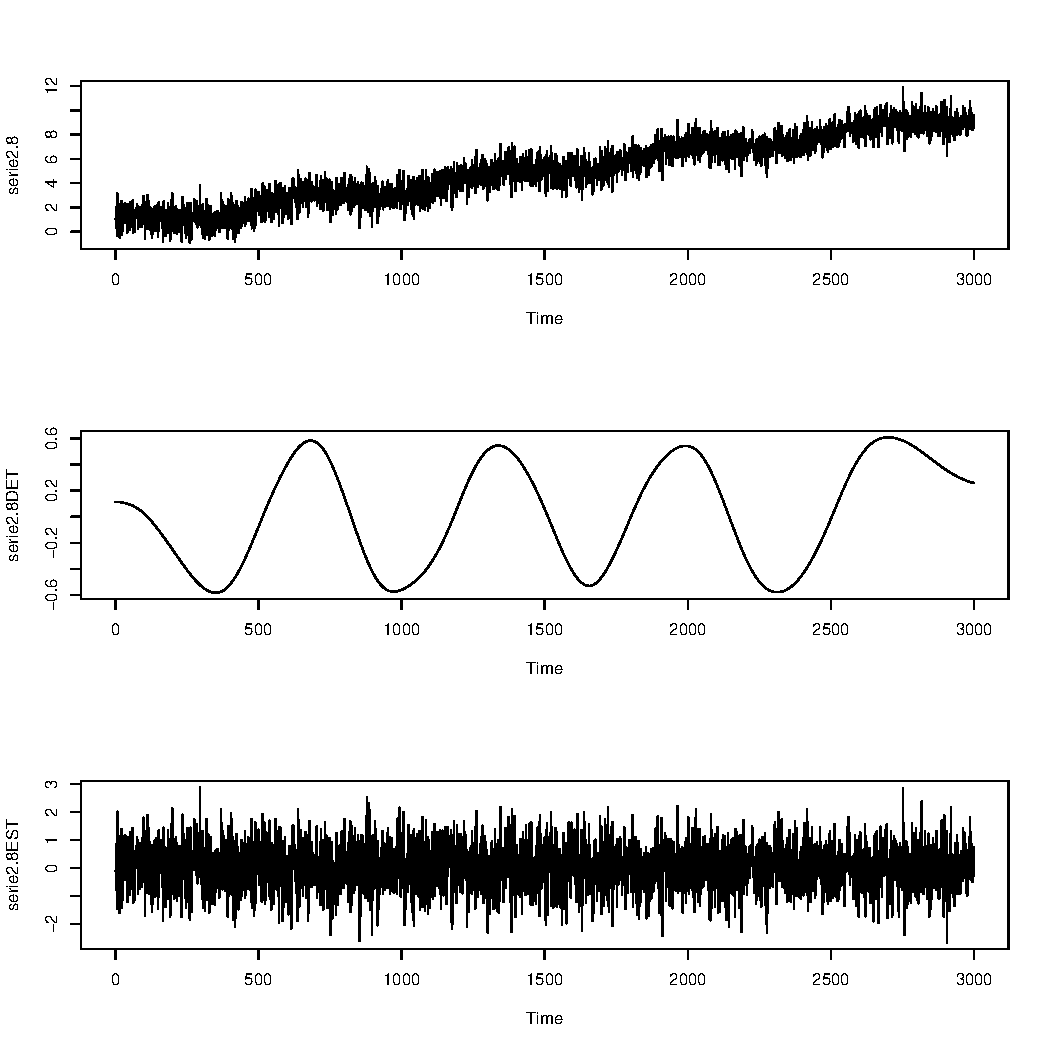
\includegraphics[scale=0.43]{serie2_8.pdf}
  \caption{Série 2.7 e Série 2.8}

\end{center}
\end{figure}

\graphicspath{{imagens/}}
\begin{figure}[H]
\begin{center}
  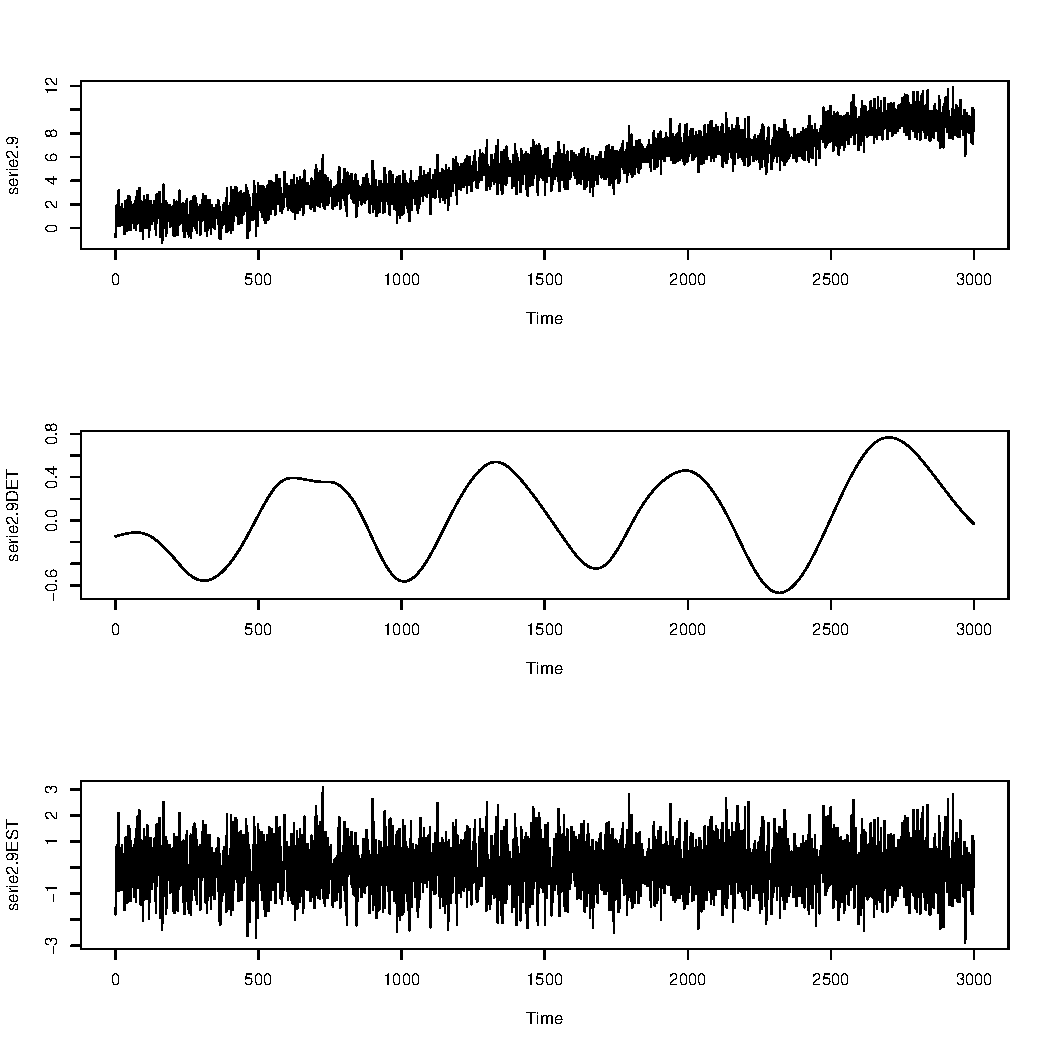
\includegraphics[scale=0.43]{serie2_9.pdf} \quad
  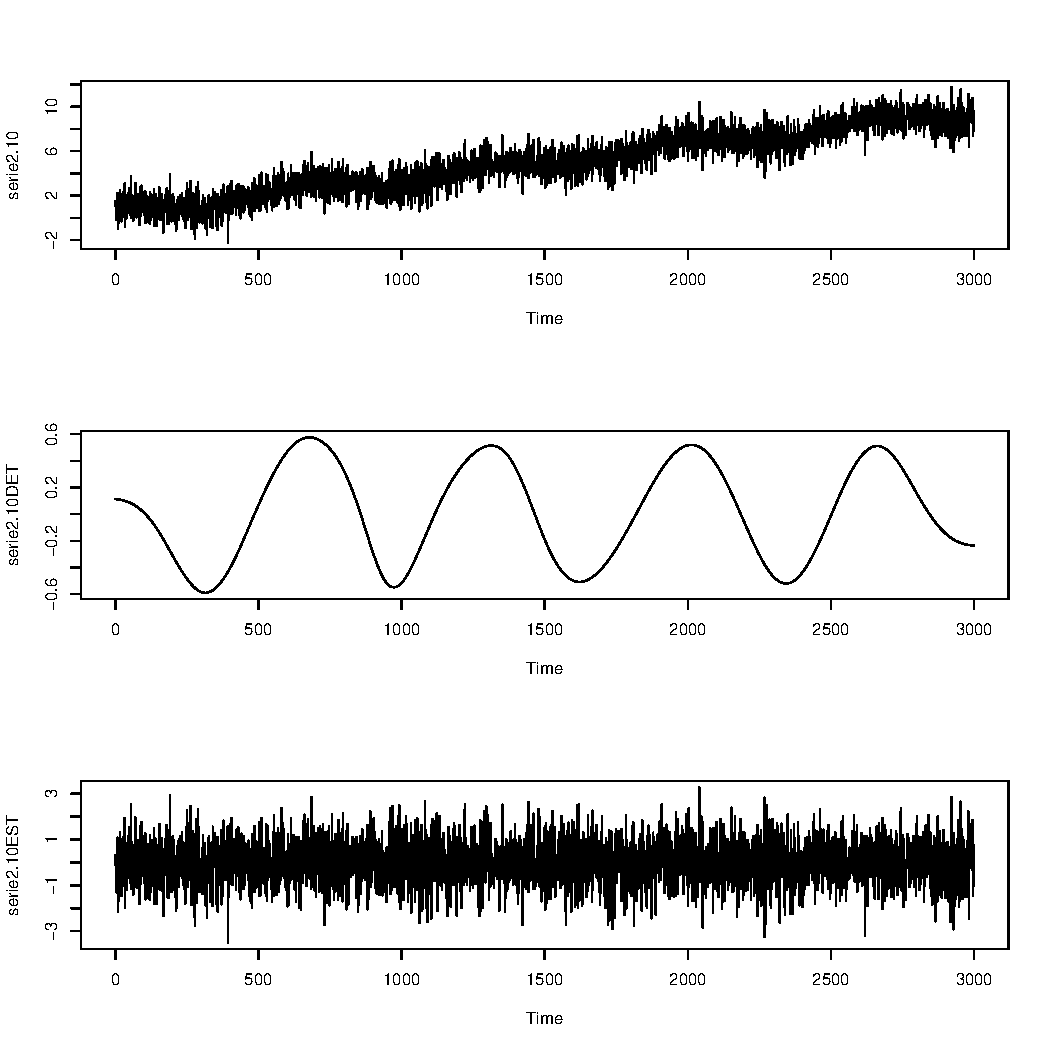
\includegraphics[scale=0.43]{serie2_10.pdf}
  \caption{Série 2.9 e Série 2.10}

\end{center}
\end{figure}

\section{Séries TIPO 3}
10 séries senoide com ruído ao longo da série.
\graphicspath{{imagens/}}
\begin{figure}[H]
\begin{center}
  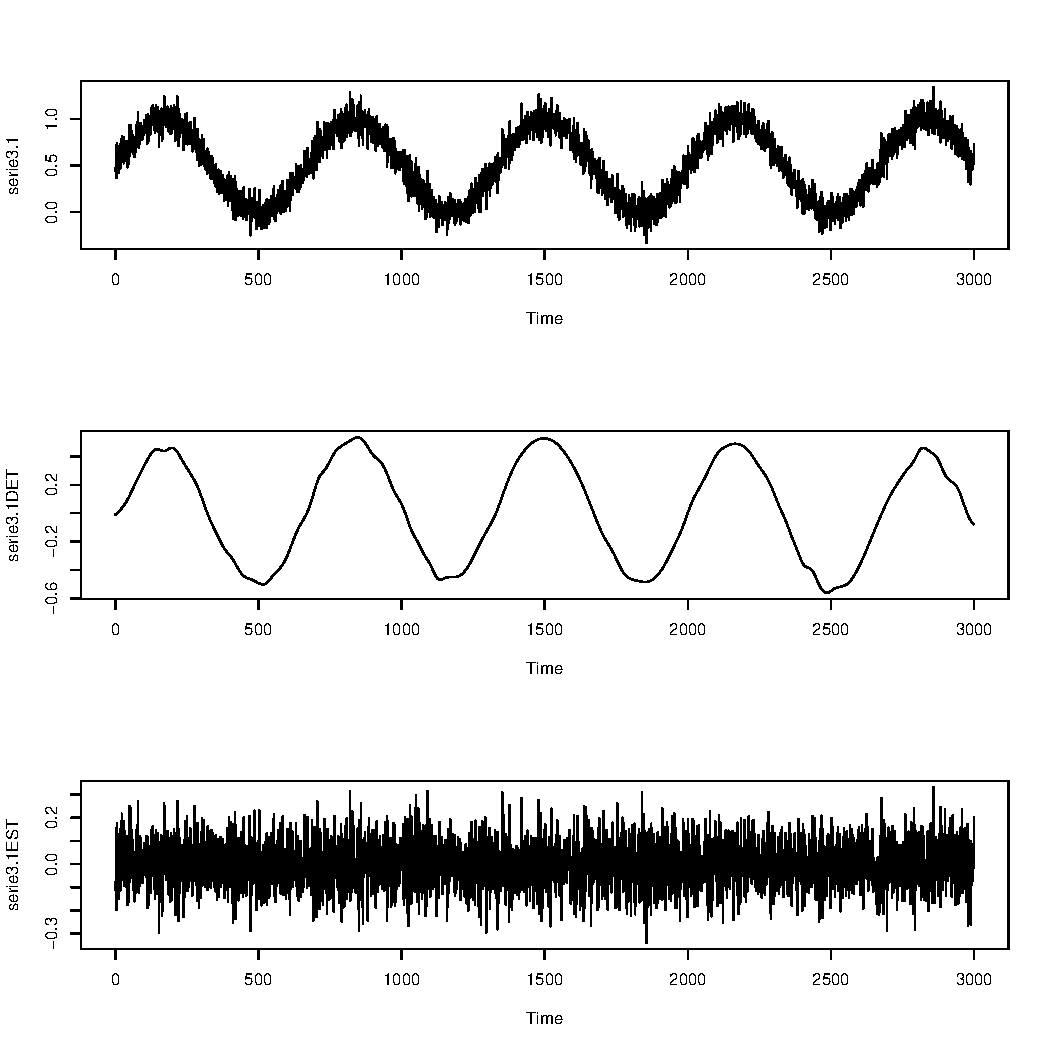
\includegraphics[scale=0.43]{serie3_1.pdf} \quad
  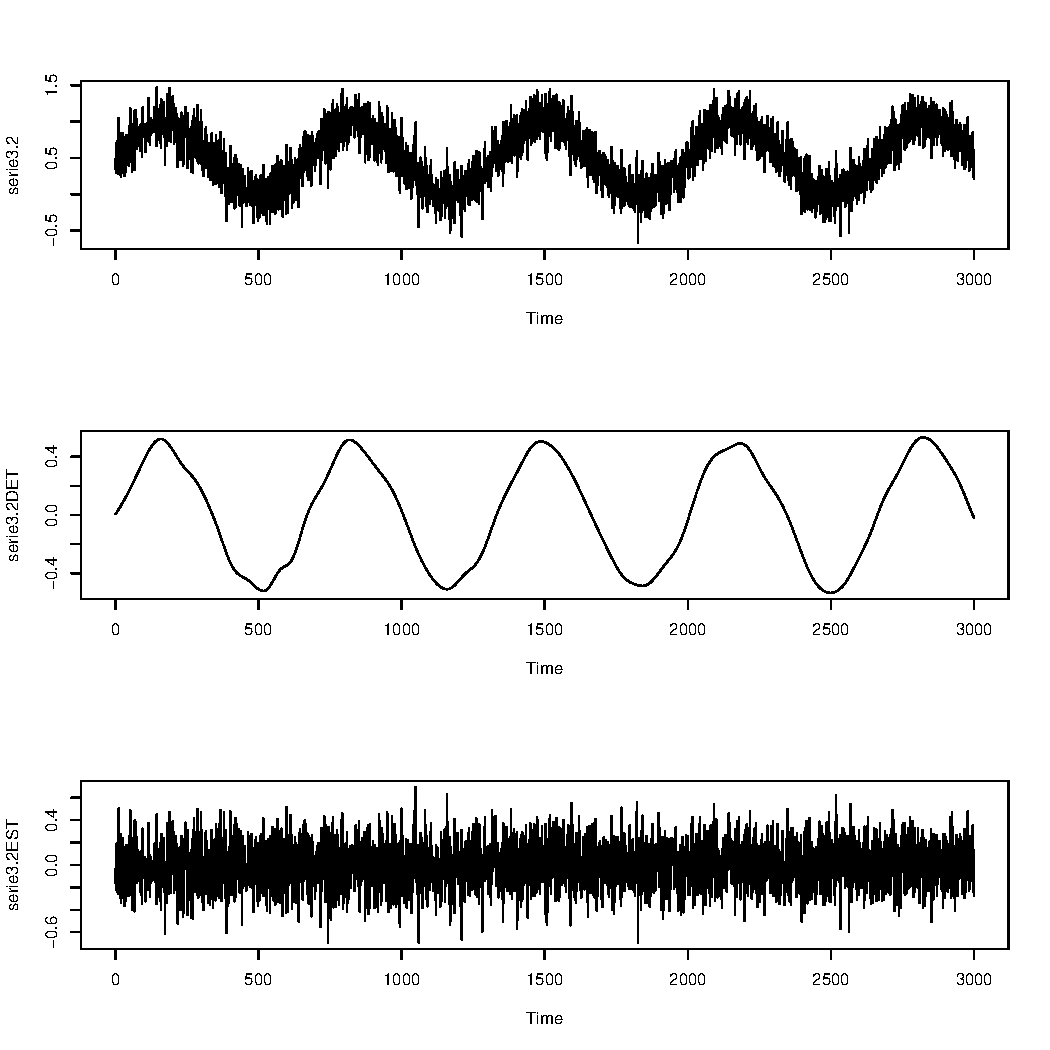
\includegraphics[scale=0.43]{serie3_2.pdf}
  \caption{Série 3.1 e Série 3.2}

\end{center}
\end{figure}

\graphicspath{{imagens/}}
\begin{figure}[H]
\begin{center}
  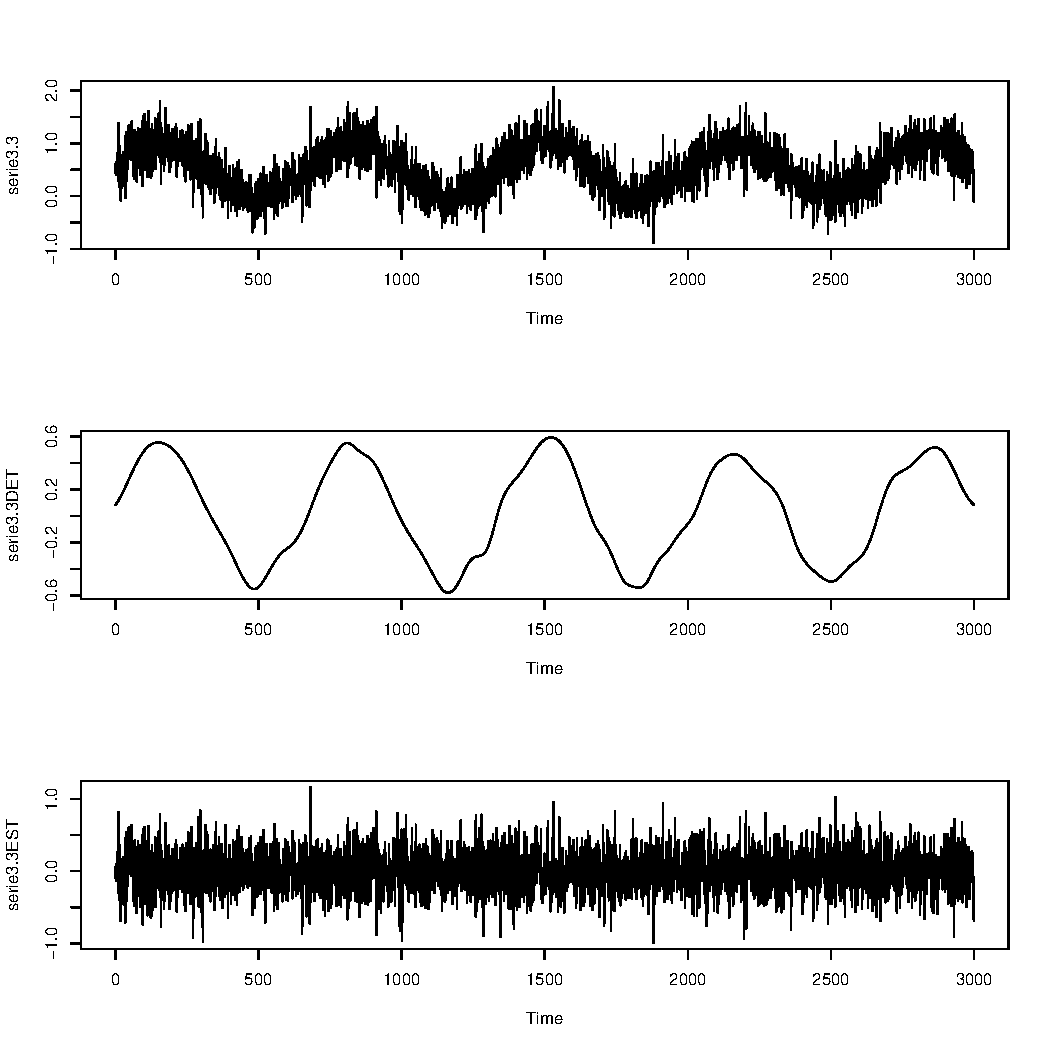
\includegraphics[scale=0.43]{serie3_3.pdf} \quad
  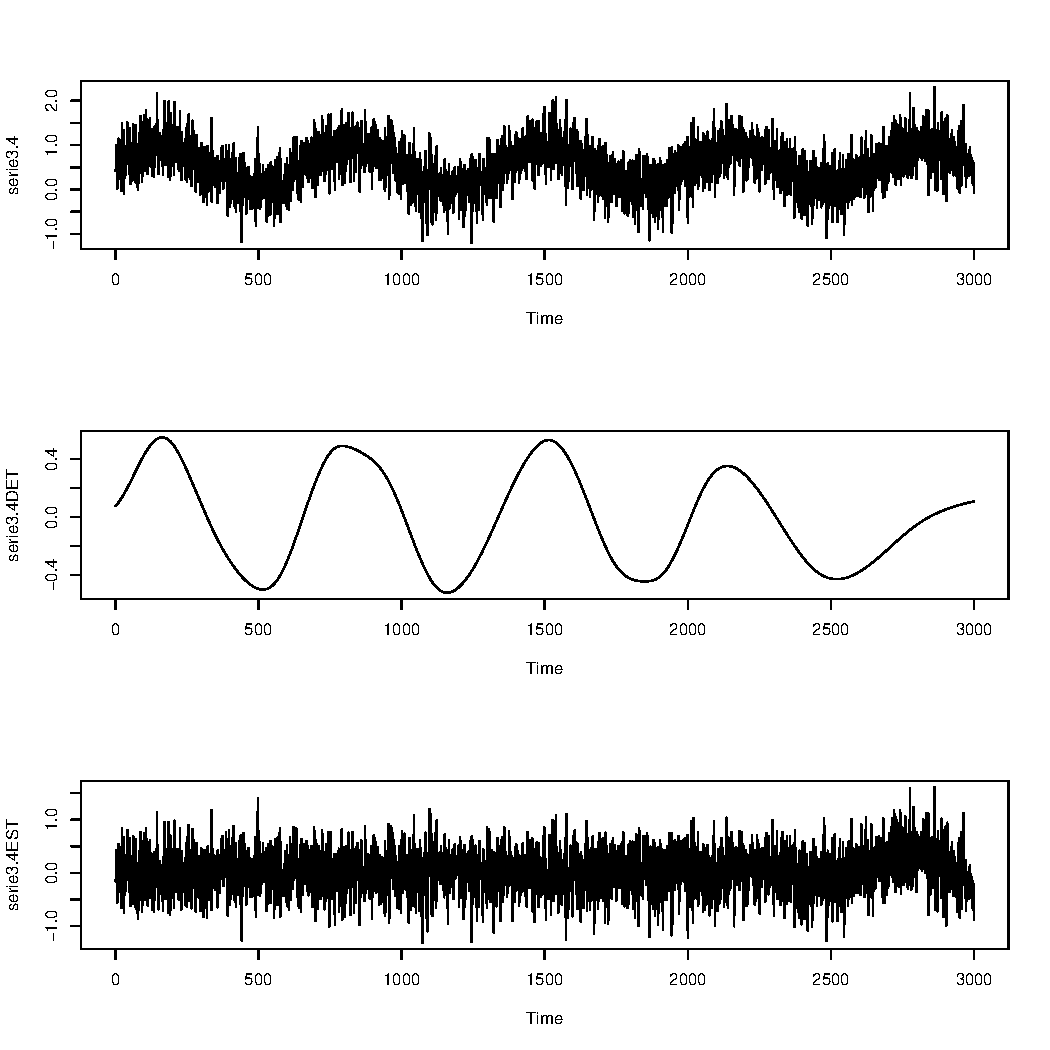
\includegraphics[scale=0.43]{serie3_4.pdf}
  \caption{Série 3.3 e Série 3.4}

\end{center}
\end{figure}

\graphicspath{{imagens/}}
\begin{figure}[H]
\begin{center}
  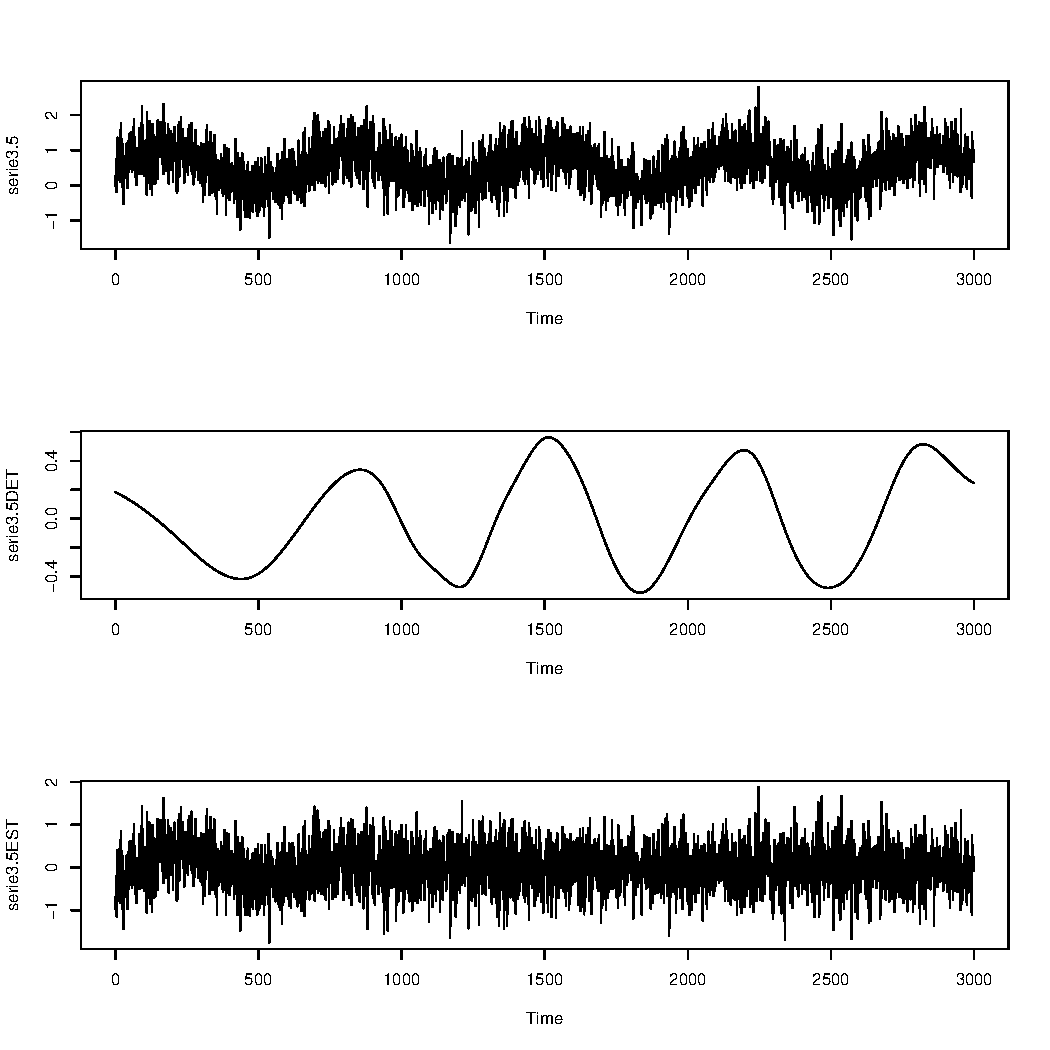
\includegraphics[scale=0.43]{serie3_5.pdf} \quad
  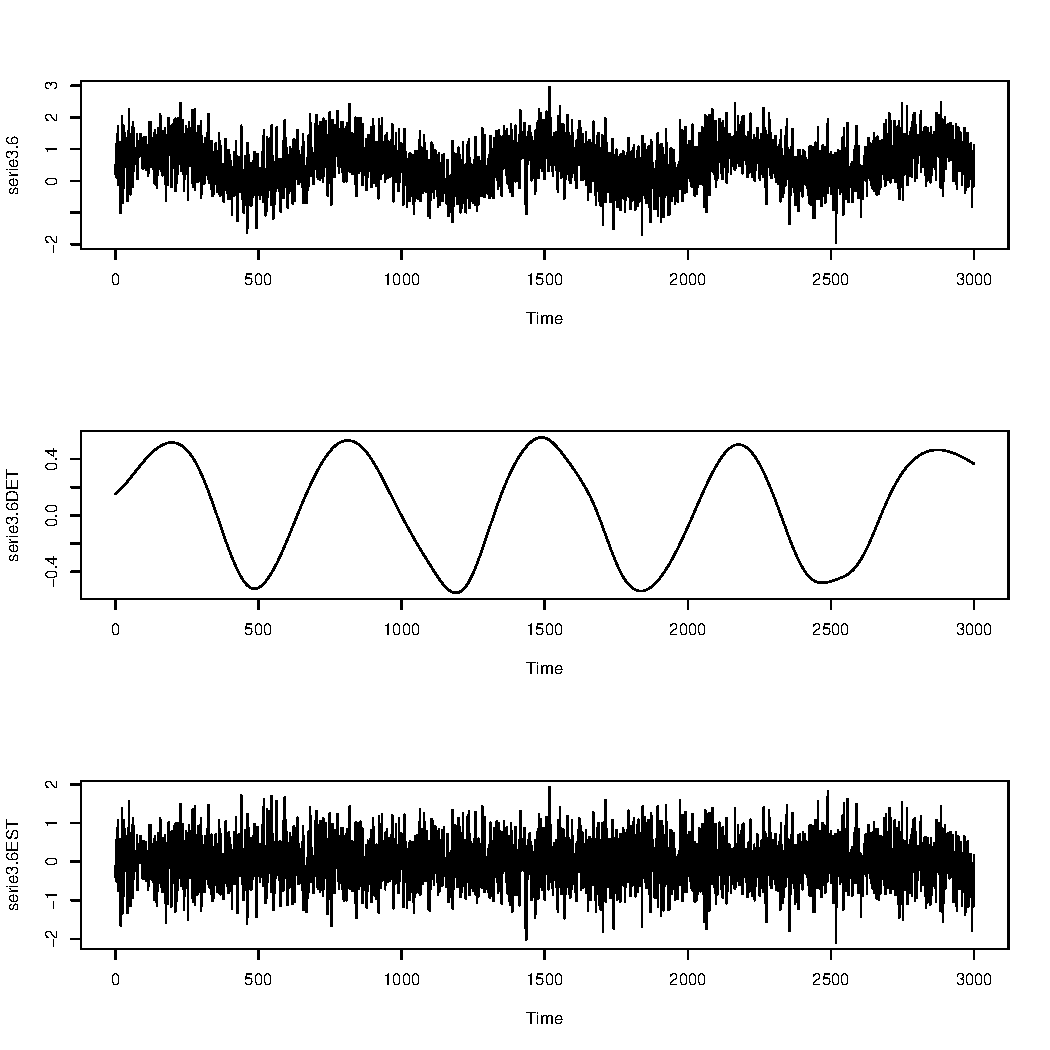
\includegraphics[scale=0.43]{serie3_6.pdf}
  \caption{Série 3.5 e Série 3.6}

\end{center}
\end{figure}

\graphicspath{{imagens/}}
\begin{figure}[H]
\begin{center}
  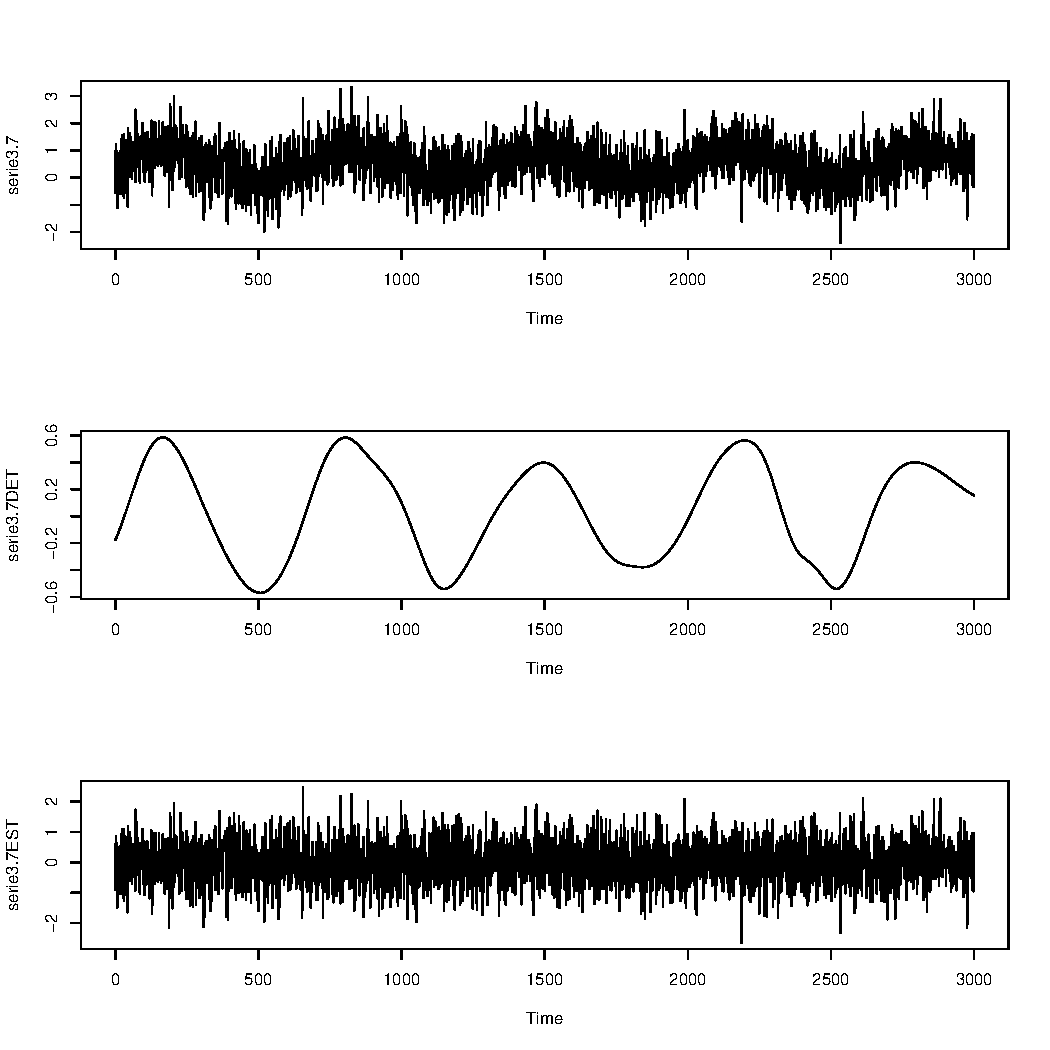
\includegraphics[scale=0.43]{serie3_7.pdf} \quad
  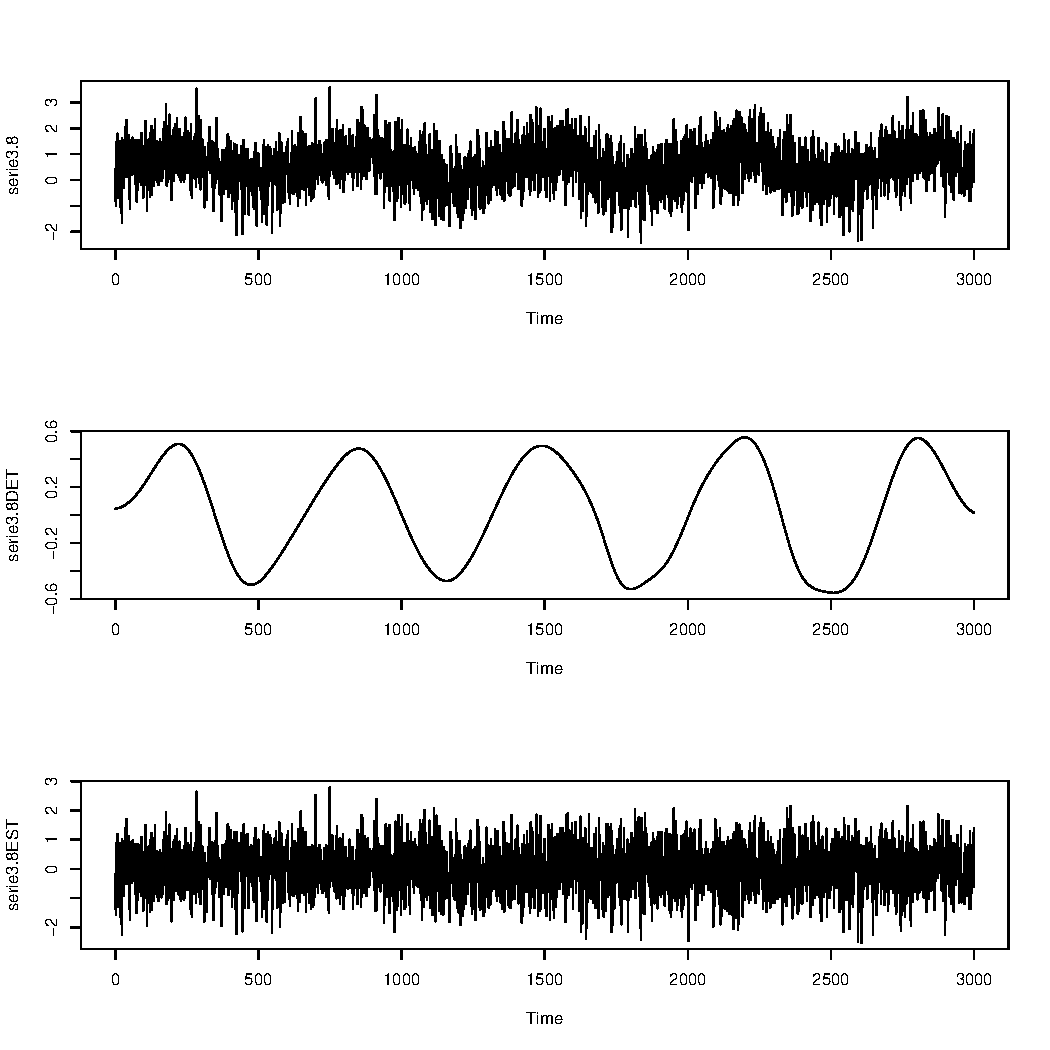
\includegraphics[scale=0.43]{serie3_8.pdf}
  \caption{Série 3.7 e Série 3.8}

\end{center}
\end{figure}

\graphicspath{{imagens/}}
\begin{figure}[H]
\begin{center}
  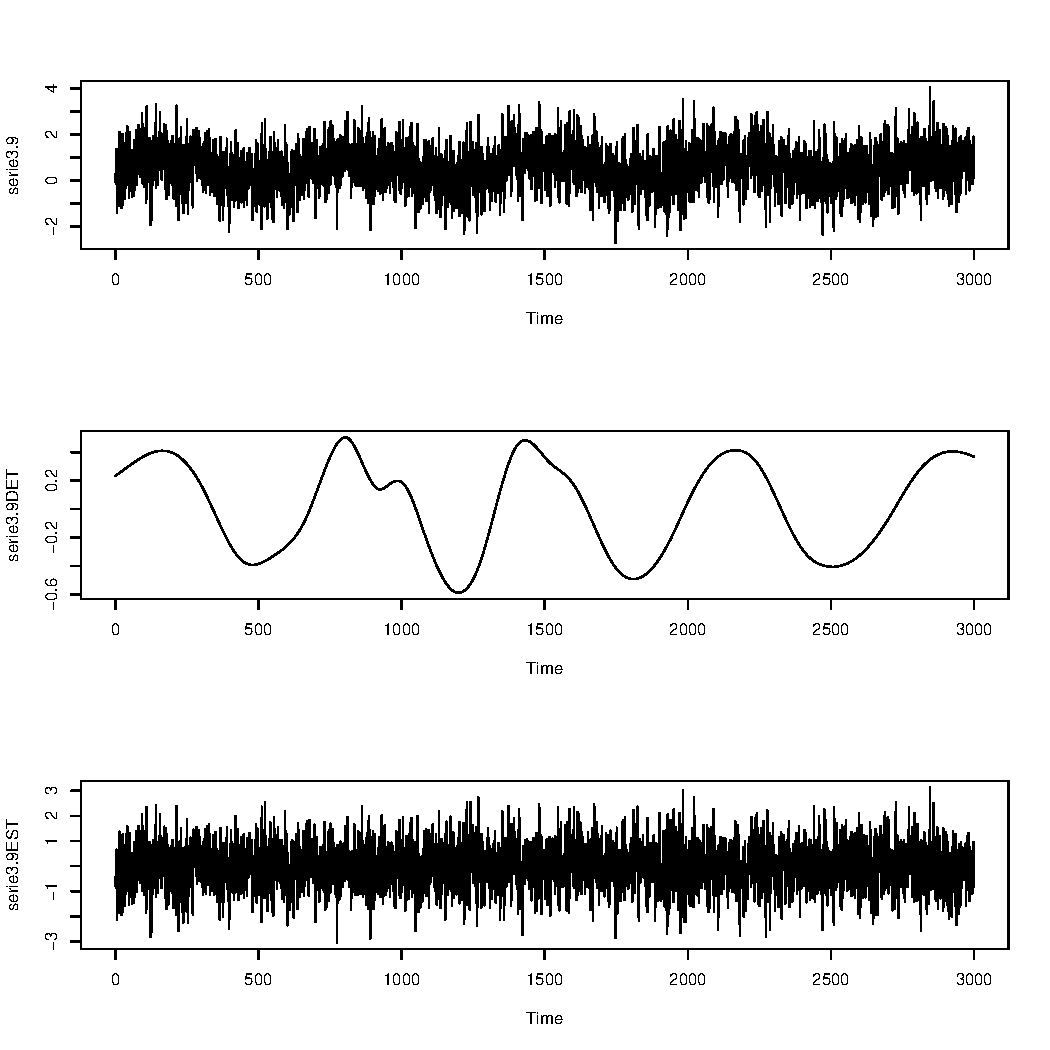
\includegraphics[scale=0.43]{serie3_9.pdf} \quad
  \includegraphics[scale=0.43]{serie3_10.pdf}
  \caption{Série 3.9 e Série 3.10}

\end{center}
\end{figure}

\section{Séries TIPO 4}
10 séries senoide com ruído ao longo da série e tendência.
\graphicspath{{imagens/}}
\begin{figure}[H]
\begin{center}
  \includegraphics[scale=0.43]{serie4_1.pdf} \quad
  \includegraphics[scale=0.43]{serie4_2.pdf}
  \caption{Série 4.1 e Série 4.2}
\end{center}
\end{figure}

\graphicspath{{imagens/}}
\begin{figure}[H]
\begin{center}
  \includegraphics[scale=0.43]{serie4_3.pdf} \quad
 \includegraphics[scale=0.43]{serie4_4.pdf}
 \caption{Série 4.3 e Série 4.4}

\end{center}
\end{figure}

\graphicspath{{imagens/}}
\begin{figure}[H]
\begin{center}
  \includegraphics[scale=0.43]{serie4_5.pdf} \quad
  \includegraphics[scale=0.43]{serie4_6.pdf}
 \caption{Série 4.5 e Série 4.6}

\end{center}
\end{figure}

\graphicspath{{imagens/}}
\begin{figure}[H]
\begin{center}
  \includegraphics[scale=0.43]{serie4_7.pdf} \quad
  \includegraphics[scale=0.43]{serie4_8.pdf}
  \caption{Série 4.7 e Série 4.8}

\end{center}
\end{figure}

\graphicspath{{imagens/}}
\begin{figure}[H]
\begin{center}
  \includegraphics[scale=0.43]{serie4_9.pdf} \quad
  \includegraphics[scale=0.43]{serie4_10.pdf}
  \caption{Série 4.9 e Série 4.10}
\end{center}
\end{figure}
\section{Considerações Finais}
Foram apresentadas as séries temporais utilizadas neste trabalho experimental e suas respactivas decomposições.
% \include{apendice2}
% ...
% \include{apendiceM}

%% Fim do documento
\end{document}
%------------------------------------------------------------------------------------------%
